% =====================================================================================================================
% CT-CORA3D — Dossier complet du projet (de l'état de l'art au code)
% Compilation : bash construire.sh   (ou : xelatex ×3 sur ce fichier)
% Pour ajouter les membres de l'équipe ou l'encadrement : modifier les commandes ci-dessous.
% =====================================================================================================================
\documentclass[11pt, a4paper, oneside, openany]{report}
% =====================================================================================================================
% preambule.tex — mise en page du dossier complet CT-CORA3D (XeLaTeX)
% Texte : Libertinus Serif. Titres, légendes, tableaux, en-têtes : Avenir Next (police livrée avec macOS ; si elle
% manque, Libertinus Sans la remplace). Code : Inconsolata. Mathématiques : Libertinus Math. Icônes : Font Awesome 5.
% Couleurs : bleu marine (titres, bandeaux), terre cuite (accents), une couleur par type d'encadré.
% =====================================================================================================================
\usepackage{mathtools}                                      % avant unicode-math
\usepackage{fontspec}
\usepackage[math-style=ISO,bold-style=ISO]{unicode-math}
\setmainfont{LibertinusSerif}[Extension=.otf, UprightFont=*-Regular, ItalicFont=*-Italic,
  BoldFont=*-Semibold, BoldItalicFont=*-SemiboldItalic, Scale=1.04]
\setmathfont{LibertinusMath-Regular.otf}[Scale=1.04]
\setmonofont{Inconsolatazi4}[Extension=.otf, UprightFont=*-Regular, BoldFont=*-Bold, Scale=MatchLowercase]
\IfFontExistsTF{Avenir Next}{%
  \setsansfont{Avenir Next}[UprightFont={* Regular}, ItalicFont={* Italic}, BoldFont={* Demi Bold},
    BoldItalicFont={* Demi Bold Italic}, Scale=MatchLowercase]
  \newfontfamily\policegrasse{Avenir Next}[UprightFont={* Bold}, Scale=MatchLowercase]
  \newfontfamily\policefine{Avenir Next}[UprightFont={* Ultra Light}, Scale=MatchLowercase]
  \newfontfamily\policemoyenne{Avenir Next}[UprightFont={* Medium}, BoldFont={* Demi Bold}, Scale=MatchLowercase]
}{%
  \setsansfont{LibertinusSans}[Extension=.otf, UprightFont=*-Regular, ItalicFont=*-Italic, BoldFont=*-Bold]
  \newfontfamily\policegrasse{LibertinusSans}[Extension=.otf, UprightFont=*-Bold]
  \newfontfamily\policefine{LibertinusSans}[Extension=.otf, UprightFont=*-Regular]
  \newfontfamily\policemoyenne{LibertinusSans}[Extension=.otf, UprightFont=*-Regular, BoldFont=*-Bold]
}
\usepackage[french]{babel}
\frenchsetup{ItemLabels=\textendash, StandardItemizeEnv=true}

\usepackage[a4paper, left=2.5cm, right=2.5cm, top=2.8cm, bottom=2.8cm, headheight=16pt, headsep=0.7cm,
  footskip=1.2cm]{geometry}
\usepackage{microtype}
\setlength{\parskip}{0.5em}
\setlength{\parindent}{0pt}
\linespread{1.08}
\emergencystretch=1.5em

% --------------------------------------------------------------------------------------------------------- couleurs
\usepackage[table]{xcolor}
\definecolor{titre}{HTML}{1B4F72}      % bleu marine : titres, bandeaux, liens
\definecolor{nuit}{HTML}{0F2B40}       % marine profond : couverture, pages de partie
\definecolor{halo}{HTML}{245A80}       % halo clair derrière le rendu de la couverture
\definecolor{accent}{HTML}{C2602A}     % terre cuite : numéros, filets, étiquettes
\definecolor{accentclair}{HTML}{F0A877}
\definecolor{encre}{HTML}{1E2832}      % couleur du texte
\definecolor{ardoise}{HTML}{55636F}    % texte secondaire (légendes, en-têtes)
\definecolor{filet}{HTML}{D3DBE2}      % filets fins
\definecolor{zebre}{HTML}{F3F6F9}      % lignes alternées des tableaux
\definecolor{entete}{HTML}{DFE9F2}     % ligne de titre des tableaux
\definecolor{segm}{HTML}{1F5F8B}       \definecolor{segmfond}{HTML}{EAF2FA}
\definecolor{planif}{HTML}{B8611A}     \definecolor{planiffond}{HTML}{FDF2E6}
\definecolor{guide}{HTML}{3A7D2C}      \definecolor{guidefond}{HTML}{EBF6E7}
\definecolor{bloc}{HTML}{6F4A99}       \definecolor{blocfond}{HTML}{F3EDF8}
\definecolor{alerte}{HTML}{B03A3A}     \definecolor{alertefond}{HTML}{FBEBEB}
\definecolor{gris}{HTML}{5B6B7A}       \definecolor{grisfond}{HTML}{F2F4F7}
\definecolor{code}{HTML}{2D3E50}       \definecolor{codefond}{HTML}{F5F7FA}
\makeatletter                                               % texte en « encre » plutôt qu'en noir pur
\AtBeginDocument{\color{encre}\let\default@color\current@color\let\XC@default@color\XC@current@color}
\makeatother

% --------------------------------------------------------------------------------------------------------- outils
\usepackage{graphicx}
\usepackage{float}
\usepackage{placeins}
\renewcommand{\topfraction}{0.85}          % une figure peut occuper presque toute la page
\renewcommand{\bottomfraction}{0.6}
\renewcommand{\textfraction}{0.1}
\renewcommand{\floatpagefraction}{0.75}
\setcounter{topnumber}{3}
\setcounter{totalnumber}{5}
\usepackage{caption}
\DeclareCaptionLabelSeparator{barre}{\enspace{\color{accent!45}\rule[-0.2em]{0.7pt}{1.05em}}\enspace}
\captionsetup{font={small,sf}, labelfont={sf,bf,color=accent}, textfont={color=ardoise}, labelsep=barre,
  margin=0.4cm, skip=8pt}
\captionsetup[table]{position=top, skip=6pt}
\usepackage{subcaption}
\usepackage{booktabs, tabularx, longtable, multirow, makecell, array}
\newcolumntype{L}[1]{>{\raggedright\arraybackslash}p{#1}}
\newcolumntype{Y}{>{\raggedright\arraybackslash}X}
\usepackage{enumitem}
\setlist{itemsep=0.2em, topsep=0.35em, parsep=0.1em}
\setlist[itemize,1]{label={\color{accent}\rule[0.1em]{0.33em}{0.33em}}, leftmargin=1.35em}
\setlist[itemize,2]{label={\color{titre}\textendash}, leftmargin=1.3em}
\setlist[enumerate,1]{label={\sffamily\bfseries\color{titre}\arabic*.}, leftmargin=1.7em}
\usepackage{siunitx}
\sisetup{locale=FR, group-minimum-digits=4}
\usepackage{pdflscape}
\usepackage{tikz}
\usetikzlibrary{calc, positioning, fadings}
\usepackage[most]{tcolorbox}
\usepackage{listings}
\usepackage{xurl}
\usepackage{fontawesome5}

% --------------------------------------------------------------------------------------------------------- tableaux
% Ligne de titre teintée (ajoutée par \toprule), lignes alternées, filets bleu marine, pas d'espace blanc autour
% des filets (sinon les lignes colorées seraient coupées).
\renewcommand{\arraystretch}{1.32}
\setlength{\aboverulesep}{0pt}
\setlength{\belowrulesep}{0pt}
\setlength{\heavyrulewidth}{0.9pt}
\setlength{\lightrulewidth}{0.5pt}
\arrayrulecolor{titre}
\let\topruleorigine\toprule
\renewcommand{\toprule}{\topruleorigine\rowcolor{entete}}
\newcommand{\titrecol}[1]{{\sffamily\bfseries\color{titre}#1}}   % texte de la ligne de titre
\AtBeginDocument{\rowcolors{2}{zebre}{white}}

% --------------------------------------------------------------------------------------------------------- titres
\usepackage[explicit]{titlesec}
\newcommand{\espacelettres}[1]{{\addfontfeature{LetterSpace=14}#1}}          % lettres espacées
\newcommand{\etiquette}[1]{{\sffamily\bfseries\addfontfeature{LetterSpace=16}\MakeUppercase{#1}}}
\newcommand{\etiquettesansnumero}{CT-CORA3D · dossier complet}
\newif\ifnumerochapitre
\newif\ifannexe
\newlength{\hauteurbandeau}
\setlength{\hauteurbandeau}{6.5cm}
% bandeau d'ouverture de chapitre : #1 étiquette (« Chapitre 6 »), #2 numéro décoratif, #3 titre
\newcommand{\bandeau}[3]{%
  \begin{tikzpicture}[remember picture, overlay]
    \coordinate (bhg) at (current page.north west);
    \coordinate (bbd) at ([yshift=-\hauteurbandeau]current page.north east);
    \fill[titre] (bhg) rectangle (bbd);
    \begin{scope}
      \clip (bhg) rectangle (bbd);
      \node[anchor=south east, inner sep=0pt, text=white, opacity=0.10,
        font=\policegrasse\fontsize{200}{200}\selectfont] at ([xshift=-1.0cm, yshift=-0.9cm]bbd) {#2};
    \end{scope}
    \fill[accent] ([yshift=-\hauteurbandeau]current page.north west) rectangle ([yshift=-2.6pt]bbd);
    \node[anchor=south west, inner sep=0pt, text width=13.6cm, text=white]   % (align=left forcerait des césures)
      at ([xshift=2.5cm, yshift=-\hauteurbandeau+1.25cm]current page.north west)
      {\raggedright{\fontsize{8.6}{11}\selectfont\color{accentclair}\etiquette{#1}}\par\vspace{9pt}%
       {\sffamily\bfseries\fontsize{25}{30.5}\selectfont #3\par}};
  \end{tikzpicture}}
\titleformat{\chapter}[block]{}{}{0pt}
  {\global\numerochapitretrue\bandeau{\chaptertitlename~\thechapter}{\thechapter}{#1}}
\titleformat{name=\chapter, numberless}[block]{}{}{0pt}
  {\global\numerochapitrefalse\bandeau{\etiquettesansnumero}{}{#1}}
\newlength{\espacebandeau}                 % espace entre le haut du texte et la fin du bandeau
\setlength{\espacebandeau}{\dimexpr\hauteurbandeau-1.95cm\relax}
\titlespacing*{\chapter}{0pt}{-\topskip}{\espacebandeau}

\newcommand{\formatsection}{\sffamily\bfseries\fontsize{15}{18.5}\selectfont\color{titre}\raggedright}
\newcommand{\formatsoussection}{\sffamily\bfseries\fontsize{12.3}{15.2}\selectfont\color{titre}\raggedright}
\titleformat{\section}{\formatsection}{\textcolor{accent}{\thesection}}{0.75em}{#1}
\titleformat{name=\section, numberless}{\formatsection}{}{0pt}{#1}
\titleformat{\subsection}{\formatsoussection}{\textcolor{accent}{\thesubsection}}{0.7em}{#1}
\titleformat{name=\subsection, numberless}{\formatsoussection}{}{0pt}{#1}
\titleformat{\subsubsection}{\sffamily\bfseries\normalsize\color{ardoise}\raggedright}{}{0em}{#1}
\titlespacing*{\section}{0pt}{1.7em}{0.55em}
\titlespacing*{\subsection}{0pt}{1.3em}{0.4em}
\titlespacing*{\subsubsection}{0pt}{1em}{0.25em}
\setcounter{secnumdepth}{2}
\setcounter{tocdepth}{1}

% premier paragraphe d'un chapitre (ce que contient le chapitre)
\newenvironment{chapeau}
  {\par\begingroup\fontsize{12.3}{17}\selectfont\color{ardoise}}
  {\par\endgroup\vspace{2pt}{\color{accent}\rule{2.4cm}{1.3pt}}\par\vspace{5pt}}

% --------------------------------------------------------------------------------------------------------- en-têtes
\usepackage{fancyhdr}
\pagestyle{fancy}
\fancyhf{}
\renewcommand{\chaptermark}[1]{\markboth{#1}{}}
\newcommand{\styleentete}{\sffamily\fontsize{8.4}{10}\selectfont}
\newcommand{\numeropage}{{\sffamily\bfseries\fontsize{9.5}{11}\selectfont\color{titre}\thepage}}
% onglet sur le bord droit de la page : sa hauteur dépend du chapitre (chapitres 1 à 14, puis annexes A à E)
\newcommand{\onglet}{%
  \ifnumerochapitre
  \begin{tikzpicture}[remember picture, overlay]
    \pgfmathsetlengthmacro{\hautonglet}{2.3cm + (\the\numexpr\ifannexe 14+\fi\value{chapter}\relax - 1)*1.33cm}
    \fill[\ifannexe accent\else titre\fi, rounded corners=3pt]
      ([xshift=-0.78cm, yshift=-\hautonglet]current page.north east) rectangle
      ([xshift=0.2cm, yshift=-\hautonglet-1.18cm]current page.north east);
    \node[text=white, font=\policegrasse\fontsize{10.5}{12}\selectfont]
      at ([xshift=-0.39cm, yshift=-\hautonglet-0.59cm]current page.north east) {\thechapter};
  \end{tikzpicture}%
  \fi}
\fancyhead[L]{\styleentete\color{ardoise}\ifnumerochapitre{\bfseries\color{accent}\thechapter}\hspace{0.7em}\fi
  \nouppercase{\leftmark}}
\fancyhead[R]{\styleentete\bfseries\color{titre}\espacelettres{CT-CORA3D}}
\fancyfoot[C]{\onglet}
\fancyfoot[R]{\numeropage}
\renewcommand{\headrulewidth}{0.4pt}
\renewcommand{\headrule}{{\color{filet}\hrule width\headwidth height\headrulewidth}}
\fancypagestyle{plain}{\fancyhf{}\fancyfoot[R]{\numeropage}\renewcommand{\headrulewidth}{0pt}}
\fancypagestyle{paysage}{\fancyhf{}\fancyfoot[R]{\numeropage}\renewcommand{\headrulewidth}{0pt}}

% --------------------------------------------------------------------------------------------------------- liens
\usepackage{hyperref}
\hypersetup{colorlinks=true, linkcolor=titre, citecolor=accent, urlcolor=segm,
  pdftitle={CT-CORA3D — Dossier complet du projet}, pdfauthor={Dorian Verstappen},
  pdfsubject={Planification CORA 3D et guides de coupe imprimables chez le chien}, pdflang={fr-FR}}
\usepackage{bookmark}
\usepackage[french, noabbrev, nameinlink]{cleveref}
\crefname{figure}{figure}{figures}            \Crefname{figure}{Figure}{Figures}
\crefname{table}{tableau}{tableaux}           \Crefname{table}{Tableau}{Tableaux}
\crefname{equation}{équation}{équations}      \Crefname{equation}{Équation}{Équations}
\crefname{chapter}{chapitre}{chapitres}       \Crefname{chapter}{Chapitre}{Chapitres}
\crefname{section}{section}{sections}         \Crefname{section}{Section}{Sections}
\crefname{subsection}{section}{sections}      \Crefname{subsection}{Section}{Sections}
\crefname{appendix}{annexe}{annexes}          \Crefname{appendix}{Annexe}{Annexes}
\creflabelformat{equation}{#2(#1)#3}

\numberwithin{equation}{chapter}

% --------------------------------------------------------------------------------------------------------- sommaire
\usepackage{etoc}
\newcommand{\pointstoc}{\leaders\hbox to 0.75em{\hss\textcolor{ardoise!55}{.}\hss}\hfill}
\newcommand{\lignetoc}[6][\hfill]{% [#1 remplissage], #2 retrait, #3 largeur du numéro, #4 numéro, #5 titre, #6 page
  {\leftskip=#2\relax \rightskip=1.3cm plus 1fil\relax \parfillskip=-\rightskip \parindent=0pt
   \noindent\llap{\makebox[#3][l]{#4}}#5\nobreak#1\nobreak\makebox[1.3cm][r]{#6}\par}}
\newcommand{\tabledesmatieres}{%
  \begingroup
  \etocsettocstyle{\chapter*{\contentsname}\markboth{\contentsname}{}}{}%
  \etocsetstyle{part}{}{\addvspace{15pt}}
    {\begingroup\hypersetup{linkcolor=white}\noindent
     \colorbox{titre}{\makebox[\dimexpr\linewidth-2\fboxsep\relax][l]{\rule[-0.6em]{0pt}{1.85em}\hspace{0.45em}%
       \etocifnumbered{{\sffamily\bfseries\fontsize{8.4}{10}\selectfont\color{accentclair}%
         \espacelettres{PARTIE~\etocthenumber}}\hspace{1.1em}}{}%
       {\sffamily\bfseries\color{white}\etocname}\hfill
       {\sffamily\bfseries\color{white}\etocpage}\hspace{0.45em}}}\par\endgroup\nobreak\addvspace{3pt}}{}%
  \etocsetstyle{chapter}{}{\addvspace{8pt}}
    {\begingroup\hypersetup{linkcolor=titre}%
     \lignetoc{1.25cm}{1.25cm}{\etocifnumbered{\policegrasse\fontsize{12.5}{14}\selectfont\color{accent}%
       \etocthenumber}{}}{\sffamily\bfseries\fontsize{11.3}{14}\selectfont\etocname}%
       {\sffamily\bfseries\color{titre}\etocpage}\endgroup\nobreak\addvspace{1pt}}{}%
  \etocsetstyle{section}{}{}
    {\begingroup\hypersetup{linkcolor=encre}%
     \lignetoc[\pointstoc]{2.35cm}{1.1cm}{\sffamily\fontsize{8.8}{11}\selectfont\color{ardoise}\etocthenumber}%
       {\fontsize{10.4}{12.8}\selectfont\etocname}%
       {\sffamily\fontsize{8.8}{11}\selectfont\color{ardoise}\etocpage}\endgroup}{}%
  \etocsettocdepth{section}%
  \tableofcontents
  \endgroup}

% --------------------------------------------------------------------------------------------------------- parties
% \partie{titre}{description} : page pleine en bleu nuit, grand numéro, description et liste des chapitres ;
% \partieannexes{description} : la même page pour les annexes (sans numéro de partie)
\newcommand{\pagepartie}[4]{% #1 étiquette, #2 grand signe décoratif, #3 titre, #4 description
  \begin{tikzpicture}[remember picture, overlay]
    \fill[nuit] (current page.south west) rectangle (current page.north east);
    \begin{scope}
      \clip (current page.south west) rectangle (current page.north east);
      \node[anchor=south east, inner sep=0pt, text=white, opacity=0.07,
        font=\policegrasse\fontsize{360}{360}\selectfont] at ([xshift=-0.8cm, yshift=-1.6cm]current page.south east)
        {#2};
    \end{scope}
  \end{tikzpicture}\par
  \vspace*{\dimexpr3.3cm-\baselineskip\relax}%
  \begingroup
  \raggedright\color{white}\hyphenpenalty=10000
  {\fontsize{9.5}{11}\selectfont\color{accentclair}\etiquette{#1}\par}%
  \vspace{12pt}%
  {\sffamily\bfseries\fontsize{29}{35}\selectfont #3\par}%
  \vspace{16pt}%
  {\color{accent}\rule{2.2cm}{2.6pt}\par}%
  \vspace{16pt}%
  {\sffamily\fontsize{12.6}{18}\selectfont\color{white!78!nuit}#4\par}%
  \vspace{1.3cm}%
  \hypersetup{linkcolor=white}%
  \etocsetstyle{chapter}{}{\addvspace{7pt}}
    {\lignetoc{1.3cm}{1.3cm}{\policegrasse\fontsize{13}{15}\selectfont\color{accentclair}\etocthenumber}%
       {\sffamily\fontsize{12.4}{15.5}\selectfont\color{white}\etocname}%
       {\sffamily\fontsize{11}{13}\selectfont\color{white!60!nuit}\etocthepage}}{}%
  \etocsettocstyle{}{}%
  \etocsetnexttocdepth{chapter}%
  \localtableofcontents
  \endgroup
  \clearpage}
\newcommand{\partie}[2]{%
  \clearpage
  \thispagestyle{empty}%
  \refstepcounter{part}%
  \addcontentsline{toc}{part}{\protect\numberline{\thepart}#1}%
  \global\numerochapitrefalse
  \pagepartie{Partie \Roman{part}}{\Roman{part}}{#1}{#2}}
\newcommand{\partieannexes}[1]{%
  \clearpage
  \thispagestyle{empty}%
  \phantomsection
  \addcontentsline{toc}{part}{Annexes}%
  \global\numerochapitrefalse
  \pagepartie{Pour aller plus loin}{A}{Annexes}{#1}}

% --------------------------------------------------------------------------------------------------------- encadrés
% Fond teinté, filet de couleur à gauche, pastille ronde avec une icône posée sur le filet.
\newcommand{\pastille}[2]{\node[circle, fill=#1, text=white, inner sep=0pt, minimum size=17pt,
  font=\fontsize{8.3}{8.3}\selectfont] at ([xshift=1.5pt, yshift=-11pt]frame.north west) {#2};}
\tcbset{
  boite/.style n args={3}{enhanced, sharp corners=west, arc=3pt, boxrule=0pt, leftrule=3pt,
    colframe=#1, colback=#2, colupper=encre, left=14pt, right=10pt, top=6pt, bottom=7pt,
    before skip=0.95em, after skip=0.95em, fonttitle=\sffamily\bfseries\small, coltitle=#1,
    attach title to upper={\par\smallskip}, parbox=false, overlay={\pastille{#1}{#3}}},
  highlight math style={enhanced, colback=accent!5, colframe=accent!55, boxrule=0.6pt, arc=3pt,
    left=7pt, right=7pt, top=4pt, bottom=4pt}}
\newtcolorbox{aretenir}[1][]{boite={segm}{segmfond}{\faLightbulb[regular]}, title={À retenir}, #1}
\newtcolorbox{danslecode}[1][]{boite={gris}{grisfond}{\faCode}, title={Dans le code}, fontupper=\small, #1}
\newtcolorbox{exemple}[1][]{boite={guide}{guidefond}{\faCalculator}, title={Exemple chiffré}, #1}
\newtcolorbox{attention}[1][]{boite={planif}{planiffond}{\faExclamationTriangle}, title={Attention}, #1}
\newtcolorbox{pourquoi}[1][]{boite={bloc}{blocfond}{\faQuestion}, title={Pourquoi ce choix ?}, #1}
% carte du guide de lecture : #1 icône, #2 lecteur
\newtcolorbox{carte}[2]{enhanced, colback=white, colframe=filet, boxrule=0.7pt, arc=4pt, left=11pt, right=11pt,
  top=10pt, bottom=10pt, fontupper=\small, colupper=encre, title={#2}, fonttitle=\sffamily\bfseries\normalsize,
  coltitle=titre, attach title to upper={\par\smallskip},
  overlay={\node[anchor=north east, text=accent!80, font=\fontsize{17}{17}\selectfont]
    at ([xshift=-10pt, yshift=-9pt]frame.north east) {#1};}}

% --------------------------------------------------------------------------------------------------------- code
\lstdefinestyle{dossier}{basicstyle=\ttfamily\small\color{code}, keywordstyle=\color{segm}\bfseries,
  commentstyle=\color{gris!90}, stringstyle=\color{planif}, numbers=none, frame=l, framerule=2.5pt,
  rulecolor=\color{titre!40}, backgroundcolor=\color{codefond}, xleftmargin=10pt, framexleftmargin=8pt,
  framextopmargin=3pt, framexbottommargin=3pt, aboveskip=0.8em, belowskip=0.8em, showstringspaces=false,
  columns=fullflexible, keepspaces=true, breaklines=true, upquote=true,
  literate={é}{{\'e}}1 {è}{{\`e}}1 {ê}{{\^e}}1 {à}{{\`a}}1 {â}{{\^a}}1 {ù}{{\`u}}1 {û}{{\^u}}1 {ô}{{\^o}}1
           {î}{{\^i}}1 {ç}{{\c c}}1 {É}{{\'E}}1 {À}{{\`A}}1 {θ}{{$\theta$}}1 {→}{{$\to$}}1 {−}{{-}}1}
\lstset{style=dossier}

% --------------------------------------------------------------------------------------------------------- macros
\newcommand{\fichier}[1]{\nolinkurl{#1}}                  % nom de fichier ou de dossier
\ExplSyntaxOn                                              % nom de fonction, de clé, de variable :
\tl_new:N \l__dossier_code_tl                              % coupure de ligne permise après chaque « _ »
\NewDocumentCommand{\code}{m}
  {
    \tl_set:Nx \l__dossier_code_tl { \tl_to_str:n {#1} }
    \regex_replace_all:nnN { \_ } { \c{textunderscore} \c{allowbreak} } \l__dossier_code_tl
    \texttt { \tl_use:N \l__dossier_code_tl }
  }
\ExplSyntaxOff
\newcommand{\vb}[1]{\symbf{#1}}                            % vecteur
\newcommand{\mt}[1]{\symbf{#1}}                            % matrice
\DeclarePairedDelimiter{\norm}{\lVert}{\rVert}
\DeclarePairedDelimiter{\abs}{\lvert}{\rvert}
\DeclareMathOperator{\atantwo}{atan2}
\DeclareMathOperator{\clamp}{clamp}
\DeclareMathOperator{\smin}{smin}
\newcommand{\dd}{\,\mathrm{d}}
\newcommand{\RR}{\mathbb{R}}
\renewcommand{\degre}{\ensuremath{^\circ}}
\newcommand{\etape}[1]{\textsf{\bfseries\color{titre}#1}}  % nom d'étape dans le texte
\newcommand{\ui}[1]{\textsf{«\,#1\,»}}                      % libellé de l'interface
\newcommand{\remarque}[1]{{\small\color{gris}#1}}

% figure sur toute la largeur, chemin relatif au dossier figures/
\graphicspath{{figures/}{figures/externes/}}
\newcommand{\fig}[4][1]{%
  \begin{figure}[htbp]\centering\includegraphics[width=#1\linewidth]{#2}\caption{#3}\label{#4}\end{figure}}
% une image d'une planche de rendus 3D : #1 hauteur, #2 image, #3 lettre, #4 légende courte
\newsavebox{\boitepanneau}
\newcommand{\panneau}[4]{%
  \sbox{\boitepanneau}{\includegraphics[height=#1]{#2}}%
  \begin{minipage}[t]{\ifdim\wd\boitepanneau<2.9cm 2.9cm\else\wd\boitepanneau\fi}\centering
    \usebox{\boitepanneau}\par\vspace{5pt}
    {\sffamily\footnotesize\color{ardoise}{\bfseries\color{accent}#3}\enspace #4\par}%
  \end{minipage}}


\newcommand{\auteurs}{Dorian Verstappen}
\newcommand{\formation}{Master en ingénierie biomédicale · ECAM Bruxelles}
\newcommand{\equipe}{Projet PMD2}
\newcommand{\referent}{Référent clinique : Anas, chirurgien vétérinaire}
\newcommand{\dateversion}{novembre 2026}

\begin{document}

% --------------------------------------------------------------------------------------------------- couverture
\begin{titlepage}
\begin{tikzpicture}[remember picture, overlay]
  \fill[nuit] (current page.south west) rectangle (current page.north east);
  % halo clair derrière le guide, puis le rendu 3D sur toute la hauteur de la page
  \shade[inner color=halo, outer color=nuit] ([xshift=-4.7cm, yshift=-13.4cm]current page.north east) circle (9.6cm);
  \node[anchor=north west, inner sep=0pt] at ([xshift=6.2cm]current page.north west)
    {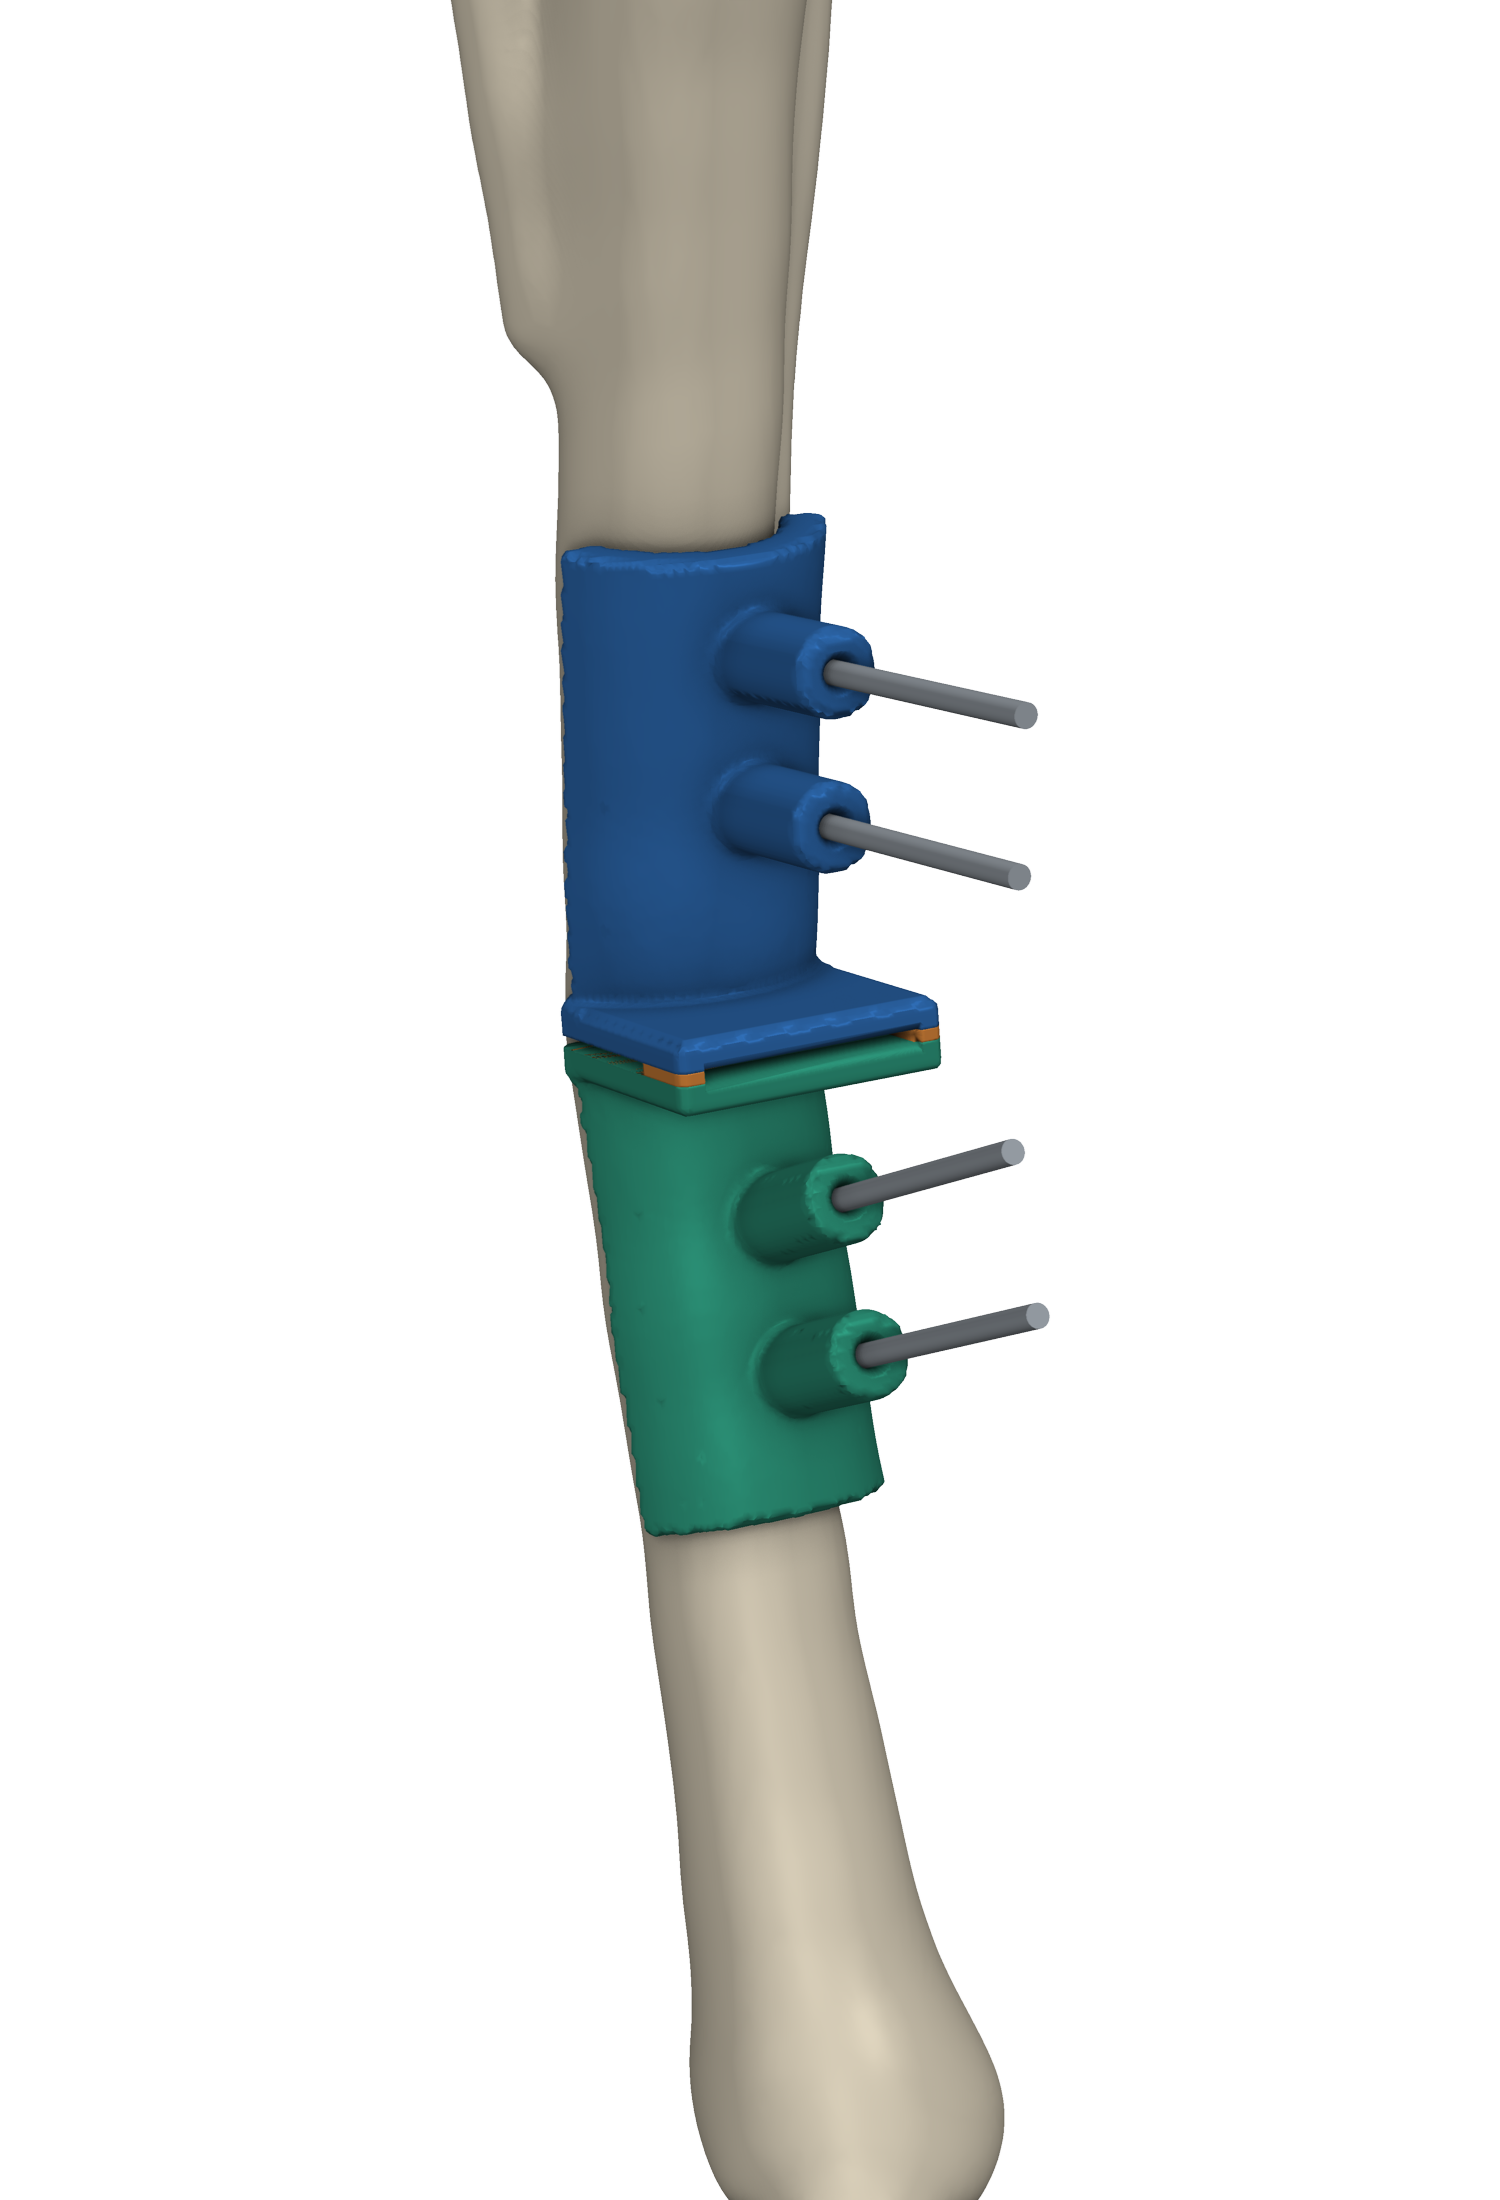
\includegraphics[height=\paperheight]{rendu_couverture.png}};
  % titre
  \node[anchor=north west, inner sep=0pt, text width=8.7cm]      % (align=left forcerait des césures)
    at ([xshift=2.1cm, yshift=-2.7cm]current page.north west)
    {\raggedright{\fontsize{8.8}{11}\selectfont\color{accentclair}\etiquette{Dossier complet du projet}}\par\vspace{16pt}
     {\policegrasse\fontsize{40}{44}\selectfont\color{white}CT-CORA3D}\par\vspace{14pt}
     {\color{accent}\rule{2.6cm}{2.6pt}}\par\vspace{16pt}
     {\sffamily\bfseries\fontsize{17}{22}\selectfont\color{white}Du scanner au guide de coupe imprimable}\par
     \vspace{9pt}
     {\sffamily\fontsize{12.5}{17}\selectfont\color{white!78!nuit}Planifier en 3D la correction\\d'un os déformé
      chez le chien}\par};
  % la chaîne en quatre temps
  \foreach \k in {1,...,4} \coordinate (e\k) at ([xshift=2.45cm, yshift=-12.6cm-(\k-1)*1.5cm]current page.north west);
  \draw[white!30!nuit, line width=1pt] (e1) -- (e4);
  \foreach \k/\t in {1/Scanner DICOM de la patte, 2/Os en 3D et repères anatomiques, 3/Planification CORA en 3D,
                     4/Guides de coupe et de réduction} {
    \node[circle, draw=accentclair, line width=1pt, fill=nuit, text=white, minimum size=21pt, inner sep=0pt,
          font=\policegrasse\fontsize{9}{9}\selectfont] (n\k) at (e\k) {\k};
    \node[anchor=west, inner sep=0pt, text=white!88!nuit, font=\policemoyenne\fontsize{11.5}{14}\selectfont]
      at ([xshift=11pt]n\k.east) {\t};
  }
  % auteur
  \node[anchor=south west, inner sep=0pt, text width=10.5cm]
    at ([xshift=2.1cm, yshift=2.3cm]current page.south west)
    {\raggedright{\sffamily\bfseries\fontsize{15}{19}\selectfont\color{white}\auteurs}\par\vspace{6pt}
     {\sffamily\fontsize{10}{14.5}\selectfont\color{white!78!nuit}\formation\\\equipe{} · \referent}\par
     \vspace{12pt}
     {\color{white!25!nuit}\rule{10.5cm}{0.5pt}}\par\vspace{7pt}
     {\sffamily\fontsize{8.6}{11}\selectfont\color{white!58!nuit}Prototype de recherche, non validé cliniquement ·
      \dateversion}\par};
\end{tikzpicture}
\end{titlepage}

\pagenumbering{roman}
\setcounter{page}{2}

% --------------------------------------------------------------------------------------------------- résumé
\chapter*{Résumé}
\addcontentsline{toc}{chapter}{Résumé}
\markboth{Résumé}{}

Quand le fémur ou le tibia d'un chien pousse de travers, le chirurgien peut couper l'os, le redresser et le fixer :
c'est une \emph{ostéotomie correctrice}. Pour savoir où couper et de combien redresser, il applique la méthode CORA
de Paley, en traçant aujourd'hui des lignes à la main sur deux radiographies. Cette préparation est longue, et une
radiographie montre mal la torsion de l'os.

CT-CORA3D fait toute cette chaîne avec un logiciel, à partir du scanner de la patte. Il lit les images DICOM, isole
chaque os en 3D, lui donne un nom, en fabrique un fichier 3D étanche, puis trouve tout seul une trentaine de repères
anatomiques sur le fémur et le tibia. Il mesure les angles articulaires, calcule en 3D le CORA, l'angle vrai de la
déformité et la correction, y compris la torsion. Il choisit ensuite une stratégie chirurgicale (coin d'ouverture ou
de fermeture, niveau de la coupe, charnière, broches) et explique chaque choix. Enfin, il construit deux pièces
prêtes à imprimer : un guide de coupe moulé sur l'os, dont les fentes guident la scie et les manchons les broches, et
un guide de réduction qui tient les fragments dans la position corrigée prévue pendant la fixation. Le tout tient dans
une application de bureau à deux onglets, pour Mac et Windows.

Nous avons testé le logiciel sur des déformités simulées dont nous connaissions la réponse : l'angle de la déformité
est retrouvé à moins d'un centième de degré, et plusieurs campagnes de simulation (606 stratégies, puis près de
1\,800 guides) passent tous les contrôles automatiques. Il reste à imprimer les guides, à les essayer sur des os
imprimés et à comparer nos planifications à celles d'un chirurgien sur de vrais patients.

Ce document explique tout le projet, de A à Z : les notions médicales, l'état de l'art, chaque calcul, chaque fichier
du code, les tests et les limites.

\section*{Abstract}
\emph{CT-CORA3D turns a computed tomography scan of a dog's hind limb into a planned corrective osteotomy and a
3D-printable, patient-specific cutting guide. The pipeline reads DICOM series, segments and names each bone, builds
watertight meshes, detects about thirty anatomical landmarks on the femur and tibia, applies Paley's CORA method in
three dimensions (true deformity angle, oblique plane, angular correction axis, derotation), chooses an opening or
closing wedge with explicit criteria, and designs the guides by implicit modelling and exact Boolean operations: a
two-part cutting guide with saw slots and pin sleeves, and a reduction guide that holds the planned correction. On simulated
deformities, the deformity angle is recovered within 0.01°, and hundreds of simulated guides pass all automatic
checks. Clinical validation remains to be done.}

% --------------------------------------------------------------------------------------------------- guide de lecture
\chapter*{Comment lire ce document}
\addcontentsline{toc}{chapter}{Comment lire ce document}
\markboth{Comment lire ce document}{}

\begin{chapeau}
Ce dossier est long, parce qu'il veut tout expliquer. Il n'est pas nécessaire de tout lire. Chaque chapitre commence
par un court paragraphe comme celui-ci, qui dit ce qu'il contient, et se termine souvent par un encadré
\emph{À retenir}.
\end{chapeau}

\section*{Par où commencer}

\begin{tcbraster}[raster columns=2, raster equal height, raster column skip=10pt, raster row skip=10pt,
  raster before skip=0.5em, raster after skip=0.7em]
\begin{carte}{\faUserMd}{Chirurgien vétérinaire}
\cref{chap:notions,chap:etat} (notions, état de l'art), \cref{sec:strategie} (stratégie chirurgicale),
\cref{sec:protocole} (mode opératoire) et \cref{chap:limites} (limites).
\end{carte}
\begin{carte}{\faChalkboardTeacher}{Enseignant, membre du jury}
Le résumé, \cref{chap:intro,chap:etat}, \cref{chap:validation} (résultats) et \cref{chap:limites}.
\end{carte}
\begin{carte}{\faUserGraduate}{Étudiant qui reprend le projet}
Tout, dans l'ordre ; puis l'\cref{ann:code}, qui décrit le code fichier par fichier.
\end{carte}
\begin{carte}{\faLaptopCode}{Développeur pressé}
\cref{chap:chaine} (vue d'ensemble), \cref{chap:application} (application), \cref{ann:code} et
\cref{ann:commandes} (commandes).
\end{carte}
\end{tcbraster}

Sur le bord droit des pages, un onglet donne le numéro du chapitre (en bleu) ou la lettre de l'annexe (en orange).
Dans la version PDF, chaque renvoi (chapitre, figure, équation, référence) est un lien cliquable.

\section*{Les encadrés}

\begin{aretenir}
L'idée principale d'une section, en quelques lignes.
\end{aretenir}
\begin{danslecode}
Le fichier et la fonction qui font ce qui vient d'être expliqué, par exemple \fichier{etape2_segmentation.py},
fonction \code{croissance()}. Les chemins sont relatifs au dossier \fichier{CT-CORA3D/}.
\end{danslecode}
\begin{exemple}
Un calcul fait avec des nombres, souvent ceux du lévrier du projet.
\end{exemple}
\begin{attention}
Un piège, une limite, ou une erreur que nous avons faite puis corrigée.
\end{attention}
\begin{pourquoi}
La raison d'un choix de conception, quand plusieurs solutions étaient possibles.
\end{pourquoi}
Les formules les plus importantes sont encadrées en orange, comme celle-ci :
\begin{equation*}
  \tcbhighmath{\tan^2\theta = \tan^2 F + \tan^2 S.}
\end{equation*}

\section*{Notations}

Les vecteurs sont en gras ($\vb{u}$, $\vb{v}$), les points en majuscules ($C$, $H$), les matrices en gras
majuscule ($\mt{R}$). Les longueurs sont en millimètres et les angles en degrés, sauf dans les formules de rotation
(radians). Le produit scalaire est noté $\vb{a}\cdot\vb{b}$ et le produit vectoriel $\vb{a}\times\vb{b}$. Les noms
de fichiers sont écrits \fichier{comme_ceci.py}, les noms de fonctions \code{comme_cela()} et les libellés de
l'interface \ui{entre guillemets}.

\begin{table}[H]
\centering\small
\begin{tabularx}{\linewidth}{L{2.6cm}Y}
\toprule
\titrecol{Symbole} & \titrecol{Signification} \\
\midrule
$X$, $Y$, $Z$ & repère de l'os : $X$ latéral, $Y$ proximal (vers le haut de l'os), $Z$ caudal (vers l'arrière) \\
$\vb{u}$, $\vb{v}$ & directions des axes des segments proximal et distal, orientées vers distal \\
$C$ & le CORA (centre de rotation de l'angulation) \\
$\theta$ & angle vrai de la déformité (en 3D) \\
$F$, $S$ & composantes frontale (vue de face) et sagittale (vue de profil) de la déformité \\
$\vb{k}$ & axe de correction (ACA) ; $\vb{b}$ : normale du plan bissecteur ; $\vb{c}$ : bissectrice transverse \\
$H$ & la charnière ; $h$ : sa profondeur dans la corticale ; $D$ : distance de la charnière à la corticale d'entrée \\
$\mt{R}$, $\mt{T}$ & rotation $3\times3$, transformation rigide $4\times4$ (rotation et translation) \\
$d(\vb{x})$ & distance signée d'un point à la surface de l'os (négative dans l'os) \\
$j$, $e$, $g$ & jeu entre l'os et le guide, épaisseur de la coque, hauteur de guidage des fentes \\
HU & unité Hounsfield (densité vue par le scanner) \\
\bottomrule
\end{tabularx}
\end{table}

\tabledesmatieres

\clearpage
\pagenumbering{arabic}

% =================================================================================================================
\partie{Le problème et ce que l'on sait}{Pourquoi un os de chien pousse de travers, comment le chirurgien le
corrige aujourd'hui, et ce que disent les publications utiles au projet.}
\chapter{Introduction}
\label{chap:intro}

\begin{chapeau}
Ce chapitre présente le problème médical, l'idée du projet et ce que fait le logiciel, en une page. Le détail vient
dans les chapitres suivants.
\end{chapeau}

\section{Le problème : un os qui pousse de travers}

Chez le chien, il arrive qu'un os de la patte arrière pousse de travers. Le fémur ou le tibia prend alors une forme
courbée ou vrillée : on parle de \emph{déformité angulaire}. Les cas les plus fréquents sont le fémur courbé vers
l'intérieur qui accompagne la luxation de la rotule, le fémur courbé vers l'extérieur des grandes races, le tibia
tordu du teckel (le \emph{pes varus}) et le tibia trop incliné vers l'avant ou vers l'arrière
\cite{brower2017,vezzoni2022,petazzoni2012}. Une déformité peut faire boiter le chien, user ses articulations ou faire
sortir sa rotule de sa place.

Pour corriger, le chirurgien fait une \emph{ostéotomie} : il coupe l'os, remet le morceau du bas dans la bonne
direction, puis le fixe avec une plaque vissée. Tout l'enjeu est de savoir \textbf{où couper, comment couper et de
combien tourner}. Une erreur de quelques degrés peut laisser une déformité, et une torsion mal corrigée peut obliger à
réopérer \cite{worth2019}.

\section{Pourquoi un scanner, et pourquoi des guides imprimés}

La méthode de référence pour préparer une ostéotomie est la méthode \emph{CORA} de Paley \cite{paley2002}. Le
chirurgien trace des lignes sur une radiographie de face et sur une radiographie de profil, puis il en déduit
l'endroit et l'angle de la coupe. Cette méthode a deux limites :
\begin{itemize}
  \item elle se fait à la main, vue par vue, alors qu'une vraie déformité est souvent \emph{oblique}, c'est-à-dire
  visible à la fois de face et de profil \cite{kim2017} ;
  \item une radiographie montre mal la \emph{torsion} de l'os : l'os vrillé sur lui-même et l'os simplement mal posé
  sur la table donnent presque la même image \cite{apelt2005,aper2005}.
\end{itemize}

Le scanner (CT, pour \emph{computed tomography}) donne l'os en trois dimensions. On y voit sa vraie forme et on peut
y mesurer la torsion \cite{dudley2006,alaiyan2021}. L'impression 3D permet en plus de fabriquer des \emph{guides
patient-spécifiques} : des pièces en plastique moulées sur l'os du patient, qui guident la scie et les broches pendant
l'opération. Plusieurs équipes vétérinaires les utilisent déjà, avec une précision de l'ordre de 2\degre{}
\cite{hall2019,jeon2023,bright2024}. Mais la préparation de ces guides se fait encore à la main, dans des logiciels de
conception, par des spécialistes.

\section{Ce que fait CT-CORA3D}

Notre objectif est de faire \textbf{toute la chaîne automatiquement}, du scanner aux pièces prêtes à imprimer, en
montrant et en expliquant chaque étape. Le chirurgien garde la décision : le logiciel propose, mesure et explique ; il
ne décide pas à sa place.

\fig{chaine_du_projet.pdf}{Les grandes étapes du projet, du scanner à la chirurgie. Les étapes 1 à 5 sont faites par
le logiciel ; la dernière est faite à la main.}{fig:chaine-projet}

Concrètement, à partir d'un dossier DICOM, le logiciel :
\begin{enumerate}
  \item reconstruit le volume du scanner et isole chaque os en 3D (segmentation), puis lui donne un nom ;
  \item fabrique un fichier 3D étanche par os (format STL, celui de l'impression 3D) ;
  \item trouve automatiquement les repères anatomiques du fémur ou du tibia et mesure ses angles articulaires et sa
  torsion ;
  \item calcule la déformité en 3D (CORA, angle vrai, plan de la déformité) et la correction ;
  \item choisit une stratégie chirurgicale : coin d'ouverture ou de fermeture, niveau de la coupe, charnière, broches,
  voie d'abord ; il explique chaque choix et le chirurgien peut tout changer ;
  \item construit deux pièces à imprimer : un guide de coupe, qui guide la scie et les broches, et un guide de
  réduction, qui tient les fragments dans la position corrigée prévue ;
  \item vérifie tout par des contrôles indépendants et écrit le mode opératoire et des plans 2D cotés.
\end{enumerate}

Tout cela tient dans une application de bureau à deux onglets : \ui{Segmentation CT} et \ui{Planification CORA}.

\section{Ce que ce projet apporte}

Les briques de base existent séparément (logiciels de segmentation, méthode CORA, guides imprimés). L'apport du projet
est de les \textbf{relier} et d'\textbf{automatiser les décisions} qui sont aujourd'hui faites à la main :
\begin{itemize}
  \item des repères anatomiques trouvés sans aide, avec les définitions des articles, et une correction de
  l'écart entre mesure 2D (radiographie) et mesure 3D (\cref{sec:calibration}) ;
  \item une méthode CORA faite en 3D, qui donne directement le coin oblique unique au lieu de deux corrections
  successives (\cref{chap:planification}) ;
  \item une stratégie chirurgicale choisie par des règles écrites et testées sur des centaines de cas
  (\cref{sec:strategie}) ;
  \item un guide conçu par modélisation implicite, qui respecte des contraintes de pose (pas de contre-dépouille, pas
  de matière entre deux os), accompagné d'un guide de réduction (\cref{chap:guides}) ;
  \item une validation systématique par des déformités simulées dont on connaît la réponse
  (\cref{chap:validation}).
\end{itemize}

\section{Le cadre}

\begin{itemize}
  \item \textbf{Projet} : PMD2, master en ingénierie biomédicale à l'ECAM Bruxelles, 2026--2027.
  \item \textbf{Données} : trois scanners d'un lévrier sain (hanche--genou, genou--cheville, pied). Les déformités
  sont donc simulées sur des os sains. Un premier cas clinique a été reçu fin octobre 2026 (\cref{sec:topogramme}).
  \item \textbf{Membre traité} : le membre pelvien (fémur et tibia). Au fémur, seulement les déformités proches du
  genou (\cref{sec:hypotheses}).
  \item \textbf{Statut} : prototype de recherche. Il ne doit pas servir sur un animal sans validation par le
  chirurgien.
\end{itemize}

\section{Plan du document}

La \textbf{partie I} pose le problème : les notions d'anatomie, de chirurgie et d'imagerie (\cref{chap:notions}),
puis l'état de l'art (\cref{chap:etat}). La \textbf{partie II} suit le chemin d'un cas, du scanner au guide : vue
d'ensemble (\cref{chap:chaine}), lecture du DICOM (\cref{chap:lecture}), segmentation (\cref{chap:segmentation}),
identification des os (\cref{chap:identification}), maillage et contrôle (\cref{chap:maillage}), repères
(\cref{chap:reperes}), planification CORA (\cref{chap:planification}) et guides (\cref{chap:guides}). Chaque chapitre
donne le principe, les calculs, puis le fichier et la fonction du code qui les font. La \textbf{partie III} décrit
l'application (\cref{chap:application}), la validation (\cref{chap:validation}), les limites et la suite
(\cref{chap:limites}). Les annexes détaillent le code fichier par fichier, tous les paramètres, le format de la
prescription, un glossaire et les commandes utiles.

\chapter{Les notions à connaître}
\label{chap:notions}

\begin{chapeau}
Ce chapitre donne le vocabulaire utilisé partout ensuite : l'anatomie du membre pelvien, la façon de décrire une
déformité, l'ostéotomie et ses outils, puis le scanner et le format DICOM. Un lecteur qui connaît déjà la chirurgie
orthopédique vétérinaire peut passer directement à la \cref{sec:scanner}.
\end{chapeau}

\section{Le membre pelvien du chien}

Le membre pelvien (la patte arrière) comprend, de haut en bas :
\begin{itemize}
  \item le \textbf{bassin}, dont la cavité (l'\emph{acétabulum}) reçoit la tête du fémur : c'est la hanche ;
  \item le \textbf{fémur}, l'os de la cuisse. En haut, sa \emph{tête} sphérique, son \emph{col} et le \emph{grand
  trochanter} ; en bas, deux \emph{condyles} séparés par l'\emph{échancrure intercondylaire}, et devant eux la
  \emph{trochlée}, la gouttière où glisse la rotule ;
  \item la \textbf{rotule} (\emph{patella}), petit os pris dans le tendon du quadriceps, et deux \textbf{fabelles},
  petits os placés derrière les condyles, dans les tendons du muscle gastrocnémien ;
  \item le \textbf{tibia}, l'os de la jambe. En haut, le \emph{plateau tibial} (deux surfaces articulaires séparées
  par l'\emph{éminence intercondylaire}) et, devant, la \emph{tubérosité tibiale}, où s'attache le tendon de la
  rotule ; en bas, la \emph{cochlée}, surface articulaire de la cheville, et la \emph{malléole médiale} ;
  \item la \textbf{fibula}, os long et fin, le long du tibia, du côté latéral et un peu en arrière ; son extrémité
  basse forme la \emph{malléole latérale} ;
  \item le \textbf{tarse} (dont le \emph{talus} et le \emph{calcanéus}), les \textbf{métatarses} et les
  \textbf{phalanges}.
\end{itemize}

Un os long a trois zones. La \emph{diaphyse} est le corps de l'os : un tube d'os dense, la \emph{corticale}, autour du
\emph{canal médullaire}. Les \emph{épiphyses} sont les extrémités, faites d'os spongieux sous une fine corticale et
recouvertes de \emph{cartilage articulaire}. Entre les deux, la \emph{métaphyse} s'élargit. Chez le jeune chien, la
\emph{physe} (cartilage de croissance) sépare épiphyse et métaphyse ; une coupe à travers une physe ouverte arrête la
croissance.

\section{Les directions et les plans}
\label{sec:directions}

En anatomie vétérinaire, on ne dit pas « devant » et « derrière », mais :
\begin{itemize}
  \item \textbf{crânial} (vers la tête, l'avant du membre) et \textbf{caudal} (vers la queue, l'arrière) ;
  \item \textbf{proximal} (vers le tronc, le haut de l'os) et \textbf{distal} (vers le pied, le bas de l'os) ;
  \item \textbf{médial} (vers le plan de symétrie du corps, l'intérieur) et \textbf{latéral} (vers l'extérieur).
\end{itemize}

Trois plans servent à regarder un os :
\begin{itemize}
  \item le \textbf{plan frontal} : on regarde l'os de face (ou de dos), comme sur une radiographie
  crânio-caudale ;
  \item le \textbf{plan sagittal} : on regarde l'os de profil, comme sur une radiographie médio-latérale ;
  \item le \textbf{plan transverse} : on regarde une coupe perpendiculaire à l'os, comme une coupe de scanner.
\end{itemize}

\begin{aretenir}
Dans tout le logiciel, chaque os est exprimé dans \textbf{son propre repère} : $X$ latéral, $Y$ proximal, $Z$ caudal,
en millimètres. Le plan frontal est donc le plan $(X, Y)$, le plan sagittal le plan $(Z, Y)$. Un membre gauche est
transformé en son image dans un miroir, pour être traité exactement comme un membre droit
(\cref{sec:repere-os}).
\end{aretenir}

\section{Décrire une déformité}
\label{sec:deformite}

\subsection{Les trois composantes}

Une déformité angulaire se décrit dans les trois plans :
\begin{itemize}
  \item \textbf{de face} : le bas de l'os part vers l'intérieur (\emph{varus}) ou vers l'extérieur (\emph{valgus}) ;
  \item \textbf{de profil} : le sommet de la courbure est en avant (\emph{procurvatum}) ou en arrière
  (\emph{recurvatum}) ;
  \item \textbf{en torsion} : le bas de l'os est tourné autour de l'axe de l'os par rapport au haut
  (\emph{torsion interne} ou \emph{externe}).
\end{itemize}

Le point où l'os change de direction s'appelle l'\emph{apex}. Une déformité à un seul apex est dite
\emph{uniapicale} ; un os tordu à deux endroits est \emph{biapical}. Ce projet traite les déformités uniapicales.

\subsection{Lignes articulaires et axes}

Pour mesurer une déformité, on trace deux sortes de lignes :
\begin{itemize}
  \item une \textbf{ligne d'orientation articulaire} (JOL, pour \emph{joint orientation line}) passe par deux repères
  d'une articulation, par exemple les points les plus bas des deux condyles du fémur ;
  \item l'\textbf{axe} d'un os ou d'un segment d'os. L'\emph{axe mécanique} relie les centres des deux articulations ;
  l'\emph{axe anatomique} suit le milieu de la diaphyse. Au tibia du chien, on utilise l'axe mécanique ; au fémur,
  l'axe anatomique \cite{tomlinson2007,dismukes2007}.
\end{itemize}

L'angle entre une ligne articulaire et l'axe est un \textbf{angle articulaire}. Son nom se lit lettre par lettre :
\textbf{m} ou \textbf{a} (axe mécanique ou anatomique), \textbf{L} ou \textbf{M} (angle mesuré du côté latéral ou
médial), \textbf{P} ou \textbf{D} (articulation proximale ou distale), \textbf{F} ou \textbf{T} (fémur ou tibia),
\textbf{A} (angle). Dans le plan sagittal, \textbf{Cr} et \textbf{Ca} (ou \textbf{Cd}) indiquent crânial et caudal.

\begin{table}[htbp]
\centering\small
\caption{Les angles articulaires utilisés par le projet.}
\label{tab:angles}
\begin{tabularx}{\linewidth}{lL{1.6cm}Y}
\toprule
\titrecol{Angle} & \titrecol{Vue} & \titrecol{Définition} \\
\midrule
aLPFA & fémur, face & entre l'axe anatomique et la ligne centre de la tête -- sommet du grand trochanter (côté latéral) \\
aLDFA & fémur, face & entre l'axe anatomique et la ligne des points distaux des condyles (côté latéral) \\
aCdDFA & fémur, profil & entre l'axe anatomique et la ligne fond de la trochlée -- milieu des points caudaux des condyles \\
mMPTA & tibia, face & entre l'axe mécanique et la ligne des centres des plateaux (côté médial) \\
mMDTA & tibia, face & entre l'axe mécanique et la ligne des sillons de la cochlée (côté médial) \\
mCaPTA & tibia, profil & entre l'axe mécanique et la ligne bords crânial -- caudal du plateau médial (côté caudal) \\
mCrDTA & tibia, profil & entre l'axe mécanique et la ligne bords crânial -- caudal de la surface distale (côté crânial) \\
\bottomrule
\end{tabularx}
\end{table}

Chez un chien sain, ces angles ont des valeurs connues, publiées pour plusieurs races (\cref{sec:normales}). Un angle
qui s'écarte de plus de deux écarts-types de la valeur normale signale une déformité. La \cref{fig:angles-reels}
montre ces angles mesurés par le logiciel sur les os du lévrier.

\section{L'ostéotomie correctrice}
\label{sec:osteotomie}

\subsection{Couper et redresser}

Pour redresser l'os, le chirurgien coupe l'os à la scie, puis il fait tourner le morceau du bas (le fragment distal)
jusqu'à ce que l'os soit droit. Deux façons de couper sont courantes (\cref{fig:coins}) :
\begin{itemize}
  \item le \textbf{coin de fermeture} : deux traits de scie retirent un petit coin d'os du côté bombé (convexe) ; on
  referme l'os. Les deux surfaces d'os restent en contact, ce qui est stable, mais l'os raccourcit un peu ;
  \item le \textbf{coin d'ouverture} : un seul trait de scie, du côté creux (concave) ; on ouvre l'os. Il s'allonge un
  peu, mais il reste un espace vide qui doit se combler (parfois avec une greffe).
\end{itemize}

\fig[0.44]{coins_fermeture_ouverture.png}{Coin de fermeture et coin d'ouverture, avant et après la correction. La
scie entre toujours du côté opposé à la charnière : c'est là que se pose le guide.}{fig:coins}

Dans les deux cas, on peut garder un petit pont d'os intact de l'autre côté : la \textbf{charnière}. Les deux
fragments tournent autour d'elle, comme autour d'une charnière de porte. La charnière apporte de la stabilité et
évite que les fragments ne glissent l'un sur l'autre. Une coupe qui traverse tout l'os est une \emph{ostéotomie
complète} : il faut alors tenir les fragments autrement, par exemple avec un guide de réduction.

\subsection{Les outils}

\begin{itemize}
  \item La \textbf{scie oscillante} a une lame fine (environ 0,6~mm) ; chaque trait enlève l'épaisseur de la lame.
  \item Les \textbf{broches de Kirschner} sont de fines tiges métalliques (ici 1,6~mm de diamètre) forées dans l'os.
  Elles fixent un guide, matérialisent une direction ou tiennent un fragment.
  \item La \textbf{plaque vissée} fixe définitivement les fragments ; chaque fragment doit recevoir au moins trois vis
  qui traversent les deux corticales.
\end{itemize}

\subsection{Les voies d'abord}

Pour atteindre l'os, le chirurgien ouvre la peau et écarte les muscles par une \emph{voie d'abord}. Toutes les faces
de l'os ne sont pas accessibles :
\begin{itemize}
  \item au \textbf{fémur}, l'abord latéral est le plus courant ; l'abord médial sert au fémur distal. Le côté crânial
  est occupé par le quadriceps et la rotule, le côté caudal par le nerf sciatique et les vaisseaux ;
  \item au \textbf{tibia}, la face médiale est sous la peau, donc facile d'accès ; la face latérale est couverte par
  les muscles crâniaux, et la fibula est derrière.
\end{itemize}
Le logiciel tient compte de ces contraintes pour décider où poser le guide (\cref{sec:abord}).

\section{Le scanner et les images DICOM}
\label{sec:scanner}

\subsection{Le principe du scanner}

Le scanner fait tourner un tube à rayons X autour de l'animal et mesure, sous des centaines d'angles, combien chaque
rayon est atténué. Un calcul de reconstruction en déduit, pour chaque petit cube de l'espace (un \emph{voxel}), un
coefficient d'atténuation $\mu$. On l'exprime en \textbf{unités Hounsfield} \cite{hounsfield1973} :
\begin{equation}
  \mathrm{HU} = 1000 \times \frac{\mu - \mu_{\text{eau}}}{\mu_{\text{eau}} - \mu_{\text{air}}}.
  \label{eq:hu}
\end{equation}
L'eau vaut donc 0~HU et l'air $-1000$~HU. Plus un tissu est dense, plus sa valeur est grande (\cref{tab:hu}).

\begin{table}[htbp]
\centering\small
\caption{Valeurs typiques au scanner (celles utilisées dans \fichier{parametres.py}).}
\label{tab:hu}
\begin{tabular}{lr}
\toprule
\titrecol{Tissu} & \titrecol{HU} \\
\midrule
air & $-1000$ \\
graisse & environ $-100$ \\
eau & 0 \\
tissus mous (muscles) & 0 à 80 \\
os spongieux & 250 à 700 \\
os cortical & 1200 à 1500 \\
\bottomrule
\end{tabular}
\end{table}

Trois défauts de l'image comptent pour la suite :
\begin{itemize}
  \item le \textbf{bruit} : deux voxels du même tissu n'ont pas exactement la même valeur. Dans les tissus mous du
  lévrier, l'écart-type mesuré est d'environ 49~HU (noyau de reconstruction osseux « BONEPLUS ») ;
  \item le \textbf{flou} : le scanner ne voit pas un bord net. Un bord d'os apparaît comme une transition progressive,
  sur environ un millimètre. Ce flou suit à peu près une courbe en cloche (gaussienne) ;
  \item l'\textbf{effet de volume partiel} : un voxel à cheval sur l'os et le tissu voisin prend une valeur
  intermédiaire. Dans une articulation serrée, quelques voxels de valeur moyenne relient deux os.
\end{itemize}

\subsection{Le format DICOM}

Un scanner est livré au format \textbf{DICOM} \cite{dicom}. Chaque coupe est un fichier qui contient l'image et un
en-tête de métadonnées. Le logiciel utilise surtout :
\begin{itemize}
  \item \code{SeriesInstanceUID} : l'identifiant de la série (un examen peut contenir plusieurs séries) ;
  \item \code{ImagePositionPatient} (IPP) : la position, en millimètres, du centre du premier pixel de la coupe ;
  \item \code{ImageOrientationPatient} (IOP) : les directions des lignes et des colonnes de l'image ;
  \item \code{PixelSpacing} : l'écart entre deux lignes et entre deux colonnes (mm) ;
  \item \code{SliceThickness} : l'épaisseur de la coupe ;
  \item \code{RescaleSlope} et \code{RescaleIntercept} : la règle qui transforme les valeurs stockées en HU.
\end{itemize}

Les positions sont données dans le \textbf{repère LPS} du patient : $x$ vers la gauche du patient
(\emph{Left}), $y$ vers l'arrière (\emph{Posterior}), $z$ vers la tête (\emph{Superior}). C'est aussi le repère des
fichiers produits par 3D Slicer \cite{fedorov2012}. Les scanners du lévrier comptent de 442 à 748 coupes de 0,625~mm.

\subsection{Topogramme ou scanner : ce qu'il faut demander}
\label{sec:topogramme}

Avant l'examen, le scanner fait une image de repérage, le \textbf{topogramme} (ou \emph{scout}) : une seule image 2D,
comme une radiographie, qui sert à choisir la zone à scanner. Elle ne suffit pas au logiciel, qui a besoin du
\textbf{volume}, c'est-à-dire de toutes les coupes.

\begin{attention}[title={Un cas vécu}]
Le premier dossier clinique reçu (27/10/2026, déformité angulaire chez un chien de 12 mois) ne contenait qu'une
image : le topogramme latéral, 512 × 512 pixels de 2~mm. À l'export, seule la première série avait été envoyée.
Aucune planification n'est possible avec une seule projection : il faut redemander l'étude complète.
\end{attention}

\begin{aretenir}[title={Ce qu'il faut demander au vétérinaire}]
\begin{itemize}
  \item l'\textbf{étude complète} en DICOM, avec toutes ses séries (pas seulement la série sélectionnée à l'écran) ;
  \item les \textbf{coupes axiales en reconstruction osseuse}, d'épaisseur 1~mm ou moins ;
  \item si possible les \textbf{deux membres} : le membre sain sert de référence pour la correction ;
  \item des fichiers \textbf{rendus anonymes} (sans nom de l'animal ni du propriétaire), et un dossier nommé par un code.
\end{itemize}
\end{aretenir}

\chapter{L'état de l'art}
\label{chap:etat}

\begin{chapeau}
Ce chapitre résume ce qui est publié et utile au projet : la méthode CORA, les valeurs normales du chien, la mesure de
la torsion, les guides imprimés, la segmentation des os et l'ostéotomie en dôme. Il se termine par la liste des
décisions que nous en avons tirées.
\end{chapeau}

\section{La méthode CORA de Paley}
\label{sec:cora-paley}

\subsection{Le principe}

La méthode de Paley \cite{paley2002} part d'une idée simple : un os déformé à un seul apex est fait de deux segments
droits. Chaque segment a son axe. On construit chaque axe à partir de la ligne articulaire de son extrémité et de
l'angle articulaire \emph{normal} : par exemple, l'axe du segment proximal du tibia est la droite qui fait l'angle
mMPTA normal (environ 93\degre{}) avec la ligne du plateau tibial. Les deux axes se croisent en un point : le
\textbf{CORA}, pour \emph{center of rotation of angulation}. L'angle entre les axes est l'angle de la déformité
$\theta$ (\cref{fig:methode-cora}).

\fig[0.8]{methode_cora.png}{Principe de la méthode CORA : (a) les axes des deux segments se croisent au CORA et font
l'angle $\theta$ ; (b) en coupant au CORA et en redressant autour de ce point, les deux axes sont de nouveau
alignés.}{fig:methode-cora}

\subsection{L'axe de correction et la bissectrice}

Redresser l'os, c'est faire tourner le segment distal de l'angle $\theta$ autour d'un axe perpendiculaire au plan de
la déformité : l'\textbf{axe de correction de l'angulation}, ou ACA. Paley montre que l'ACA doit se trouver sur la
\textbf{bissectrice transverse} du CORA, la droite qui partage en deux l'angle entre les axes, dans le plan de la
déformité. C'est la seule façon de réaligner les axes sans translation. La position de l'ACA le long de la bissectrice
choisit le type de coin :
\begin{itemize}
  \item ACA sur la corticale concave : \textbf{coin de fermeture} (l'os raccourcit) ;
  \item ACA sur la corticale convexe : \textbf{coin d'ouverture} (l'os s'allonge) ;
  \item ACA au milieu de l'os : \textbf{coin neutre} (une moitié se ferme, l'autre s'ouvre ; la longueur change peu).
\end{itemize}

\subsection{Les règles d'ostéotomie}

Paley énonce trois règles, selon l'endroit de la coupe par rapport au CORA :
\begin{itemize}
  \item \textbf{règle 1} : la coupe et l'ACA passent par le CORA. Les axes sont réalignés, sans translation ;
  \item \textbf{règle 2} : la coupe est faite à un autre niveau, mais l'ACA reste au CORA. Les axes sont réalignés,
  et le fragment distal glisse le long de la coupe : c'est une \emph{translation à l'ostéotomie} ;
  \item \textbf{règle 3} : la coupe et l'ACA sont loin du CORA. L'angle est corrigé, mais les axes restent décalés :
  il reste une translation de l'axe, à éviter.
\end{itemize}
On utilise la règle 2 quand on ne peut pas couper au CORA, par exemple parce qu'il est trop près de l'articulation.
Notre logiciel applique la règle 1 par défaut et passe à la règle 2 si le trait de coupe serait trop près du
cartilage (\cref{sec:regle2}).

\subsection{Le plan oblique et l'angle vrai}
\label{sec:oblique}

Une déformité réelle est rarement pure. Le plus souvent, elle a une composante de face $F$ et une composante de profil
$S$ : elle se trouve dans un plan \emph{oblique}. L'angle vrai n'est pas la somme des deux, et corriger les deux vues
l'une après l'autre reviendrait à mal corriger. Quand l'axe proximal est vertical, Paley donne
\begin{equation}
  \tan^2\theta = \tan^2 F + \tan^2 S,
  \qquad
  \tan\varphi = \frac{\abs{\tan S}}{\abs{\tan F}},
  \label{eq:oblique}
\end{equation}
où $\varphi$ est l'orientation du plan de la déformité par rapport au plan frontal \cite{paley2002,qatu2024}. Pour
$F = 15\degre$ et $S = 10\degre$, on trouve $\theta = 17{,}8\degre$, et non 25\degre. Une seule ostéotomie oblique
corrige alors les deux composantes à la fois \cite{kim2017}. La démonstration est donnée à la \cref{sec:angle-vrai}.

\section{Les valeurs normales chez le chien}
\label{sec:normales}

Les valeurs normales des angles articulaires viennent de radiographies de chiens sains, surtout de grandes races
(\cref{tab:normales}). Deux points comptent :
\begin{itemize}
  \item \textbf{la race compte}. L'aLDFA normal va de 94 à 98\degre{} selon la race \cite{tomlinson2007} ; l'équipe
  Vezzoni retient 94 ± 3,3\degre{} (berger allemand) comme borne de normalité \cite{vezzoni2022}. Une étude au
  scanner compare six races \cite{bruhschwein2023r} ;
  \item \textbf{la définition compte}. Ces valeurs sont mesurées sur des radiographies, avec des repères placés par un
  observateur. Un logiciel qui mesure en 3D avec ses propres repères ne trouve pas exactement le même angle sur le même
  os. Nous corrigeons cet écart de définition (\cref{sec:calibration}).
\end{itemize}

\begin{table}[htbp]
\centering\small
\caption{Valeurs normales publiées (moyenne ± écart-type) utilisées par le logiciel. En gras : la référence par
défaut (travaux de l'équipe Vezzoni, sinon la littérature).}
\label{tab:normales}
\begin{tabularx}{\linewidth}{lL{2.6cm}Y}
\toprule
\titrecol{Angle} & \titrecol{Valeur} & \titrecol{Source} \\
\midrule
aLPFA & 103 ± 6,4\degre & Tomlinson 2007, Labrador \cite{tomlinson2007} \\
aLDFA & \textbf{94 ± 3,3\degre} & Vezzoni 2022 (valeur du berger allemand de Tomlinson 2007) \cite{vezzoni2022} \\
 & 97 ± 3,2\degre & Tomlinson 2007, Labrador \cite{tomlinson2007} \\
aCdDFA & 90,5 ± 6,3\degre & Kara 2018, scanner 3D, définition voisine \cite{kara2018} \\
mMPTA & \textbf{93,3 ± 1,78\degre} & Olsen, Vezzoni 2016 (= Dismukes 2007) \cite{olsen2016,dismukes2007} \\
mMDTA & 96,0 ± 2,7\degre & Dismukes 2007 \cite{dismukes2007} \\
mCaPTA & \textbf{63,7 ± 2,6\degre} & Guénégo, Vezzoni 2021 : 90\degre{} − pente du plateau (26,3\degre) \cite{guenego2021} \\
mCrDTA & 81,6 ± 3,2\degre & Dismukes 2008, radiographie de profil \cite{dismukes2008s} \\
valgus tibial & 11,8 ± 3,1\degre & cité par IMAIOS \cite{imaios} \\
pente du plateau (TPA) & 22,5\degre & lévrier sain, « à considérer comme normal » \cite{wilke2002} \\
\bottomrule
\end{tabularx}
\end{table}

\section{Mesurer la torsion}
\label{sec:etat-torsion}

La torsion est l'angle, autour de l'axe long de l'os, entre un axe transverse proximal et un axe transverse distal.
Au fémur, on parle d'\emph{antéversion} : l'angle entre l'axe du col et la ligne qui passe derrière les condyles.

\begin{itemize}
  \item \textbf{La radiographie ne suffit pas}. Elle ne distingue pas une torsion de l'os d'une simple rotation du
  membre sur la table \cite{apelt2005,aper2005}, et une rotation du fémur change à elle seule l'aLDFA mesuré
  \cite{miles2016}.
  \item \textbf{Le scanner mesure la torsion} \cite{dudley2006,mostafa2014}. Al Aiyan et al. trouvent une
  antéversion de 31 ± 5\degre{} chez 58 chiens de races moyennes et grandes \cite{alaiyan2021}. Brühschwein et al.
  proposent un repère 3D centré sur l'os, exact sur un modèle de torsion \cite{bruhschwein2023f}, et l'appliquent au
  tibia \cite{bruhschwein2023t}.
  \item \textbf{Seuils} : Longo et al. planifient des ostéotomies de dérotation en 3D et donnent des seuils de torsion
  anormale \cite{longo2022}.
  \item \textbf{Au bloc}, contrôler la rotation à l'œil ou à la radioscopie est imprécis : 4 à 9\degre{} d'erreur
  moyenne dans une étude sur cadavre \cite{ivanov2024} ; les signes radiographiques classiques ont leurs limites
  \cite{krettek1998,fang2015}.
\end{itemize}

\begin{attention}[title={Les conventions de signe varient}]
Selon les articles, une même torsion est dite « interne » ou « externe », et son signe change. Le logiciel suit les
Méthodes de Longo 2022 pour le tibia ($-$ = interne, $+$ = externe ; normale vers $-4\degre$, anormale en dessous de
$-10\degre$ ou au-dessus de $+2\degre$) et l'antéversion d'Al Aiyan 2021 pour le fémur ($+$ = col dirigé vers
crânial ; normale 31 ± 5\degre). Le résumé de l'article de Longo inverse les deux mots : il faut lire les Méthodes.
\end{attention}

\section{Planification virtuelle et guides imprimés}
\label{sec:etat-guides}

Plusieurs équipes ont publié des corrections planifiées sur ordinateur et réalisées avec des guides imprimés en 3D
(\cref{tab:guides}). Ces résultats portent sur toute la chaîne : préparation, guide et geste chirurgical.

\begin{table}[htbp]
\centering\small
\caption{Guides imprimés chez le chien : ce qui est publié.}
\label{tab:guides}
\begin{tabularx}{\linewidth}{L{2.6cm}L{3.2cm}Y}
\toprule
\titrecol{Étude} & \titrecol{Os, système} & \titrecol{Résultat} \\
\midrule
Worth 2019 \cite{worth2019} & avant-bras ; guides de coupe seuls & 1 membre sur 7 réopéré pour une rotation mal corrigée \\
Hall 2019 \cite{hall2019} & fémur distal (luxation de rotule) ; coupe + réduction & torsion à 1,7 ± 2,1\degre{} de la cible \\
Carwardine 2021 \cite{carwardine2021} & avant-bras ; coupe, repositionnement, plaques en titane & plaque sur mesure, trous percés à travers le guide \\
De Armond 2022 \cite{dearmond2022} & avant-bras, 1 ou 2 apex ; coupe + réduction & plus de 90~\% des paramètres à moins de 5\degre{} et 5~mm \\
Jeon 2023 \cite{jeon2023} & tibia de petites races & erreurs de 1,8 (profil), 2,3 (face) et 2,6\degre{} (torsion) \\
Bright 2024 \cite{bright2024} & tibia du teckel (pes varus) & moins de 2\degre{} et 1~mm dans tous les plans \\
\bottomrule
\end{tabularx}
\end{table}

Deux leçons en ressortent. D'abord, un guide de coupe seul contrôle mal la rotation ; il faut un moyen de
\textbf{remettre les fragments à la bonne place} après la coupe : un guide de réduction qui s'enfile sur des broches,
ou une plaque sur mesure. Ensuite, l'erreur finale est de l'ordre de \textbf{2\degre} : c'est l'objectif à viser, et
l'erreur du calcul doit être bien plus petite.

\section{Le choix du coin dans la pratique}
\label{sec:etat-coin}

Les publications donnent des stratégies types :
\begin{itemize}
  \item \textbf{pes varus du teckel} : coin d'ouverture médial au CORA, en gardant la corticale latérale comme
  charnière \cite{petazzoni2012} ;
  \item \textbf{varus du fémur distal} (luxation médiale de la rotule) : coin de fermeture latéral ; l'aLDFA passe de
  107,6 à 94,1\degre{} \cite{brower2017} ;
  \item \textbf{valgus du tibia proximal} : coin de fermeture médial associé à une TPLO ; le mMPTA passe de 101 à
  92,8\degre{} \cite{vezzoni2020} ;
  \item \textbf{pente du plateau tibial} : coin de fermeture crânial (CCWO), dont l'angle est relié à la pente
  \cite{guenego2021,guenego2025}. Un coin d'ouverture modifie facilement la pente : 1~mm d'erreur d'ouverture en avant
  change la pente d'environ 2\degre{} \cite{noyes2005,ducat2012}.
\end{itemize}

\section{La segmentation des os au scanner}
\label{sec:etat-segmentation}

Segmenter, c'est décider pour chaque voxel à quel os il appartient. Trois familles de méthodes sont utiles ici :
\begin{itemize}
  \item le \textbf{seuillage} : on garde les voxels au-dessus d'une valeur. Le seuil « Bone (CT) » du logiciel
  Mimics, 226~HU, est très utilisé en planification 3D. Mais à ce seuil, les os d'une articulation se touchent (volume
  partiel) et forment un seul bloc ;
  \item la \textbf{croissance de région} : on part d'un point (une graine) et on ajoute les voxels voisins qui
  ressemblent ;
  \item la \textbf{ligne de partage des eaux} (\emph{watershed}) \cite{meyer1994} : on voit l'image comme un relief
  et on le remplit d'eau depuis des sources ; les frontières sont là où deux eaux se rencontrent.
\end{itemize}
Le logiciel libre 3D Slicer \cite{fedorov2012} offre ces outils à la main. La surface 3D est ensuite extraite par
l'algorithme des \emph{marching cubes} \cite{lorensen1987}. Notre méthode (\cref{chap:segmentation}) combine un seuil
qui monte pour trouver une graine par os, puis une croissance de région compétitive.

\section{L'ostéotomie en dôme}
\label{sec:dome}

Quand on ne peut pas couper au CORA et qu'on veut éviter la translation de la règle 2, on peut faire une coupe
courbe, un cylindre centré sur le CORA : les fragments tournent l'un sur l'autre le long de cette coupe, sans
translation, en restant en contact. Elle est décrite au radius du chien, pour une ou deux déformités
\cite{fox2006}.

\begin{pourquoi}
Nous ne proposons pas le dôme : (1) il faut une lame courbe de rayon fixe et un guide qui fasse tourner la lame autour
d'un pivot, plus difficile à imprimer et à contrôler qu'une fente plane ; (2) un dôme cylindrique ne tourne qu'autour
de son axe : il corrige l'angle mais pas la torsion ; (3) au fémur distal et au tibia, le CORA est le plus souvent dans
une zone où la règle 1 est possible.
\end{pourquoi}

\section{Ce que nous en retenons}
\label{sec:retenu}

\begin{aretenir}[title={Les décisions du projet, tirées de l'état de l'art}]
\begin{enumerate}
  \item Partir du \textbf{scanner}, pour avoir la forme 3D et la torsion (\cref{chap:lecture}).
  \item Trouver les \textbf{repères automatiquement}, avec les définitions des articles, et corriger l'écart entre
  la mesure 2D publiée et notre mesure 3D (\cref{chap:reperes}).
  \item Faire la méthode CORA \textbf{en 3D} : un seul coin oblique, l'ACA sur la bissectrice, la règle 1 par défaut
  (\cref{chap:planification}).
  \item Corriger la \textbf{torsion} par une dérotation, avec les définitions publiées au scanner.
  \item Choisir le coin et la voie d'abord par des \textbf{règles explicites}, conformes aux pratiques publiées
  (\cref{sec:strategie}).
  \item Ne pas se contenter d'un guide de coupe : prévoir un \textbf{moyen de réduction} qui contrôle la rotation
  (guide de réduction, \cref{chap:guides}).
  \item Viser une erreur de calcul très inférieure aux \textbf{2\degre} publiés, et le vérifier sur des cas simulés
  (\cref{chap:validation}).
\end{enumerate}
\end{aretenir}


\partie{Du scanner au guide : les méthodes et les calculs}{Chaque étape du logiciel, dans l'ordre : lire le
scanner, séparer et nommer les os, fabriquer les surfaces, trouver les repères, planifier la correction en 3D, puis
construire le guide de coupe. Chaque calcul est expliqué et démontré.}
\chapter{La chaîne de calcul en un coup d'œil}
\label{chap:chaine}

\begin{chapeau}
Ce chapitre donne la carte de la partie II : les étapes, les fichiers qu'elles échangent, les repères dans lesquels
on calcule, les données du projet et les hypothèses de travail.
\end{chapeau}

\section{Les étapes et les fichiers}

La \cref{fig:chaine-complete} montre le chemin d'un cas. Les étapes 1 à 6 sont écrites en Python (dossier
\fichier{code_source/}). La planification CORA est écrite en JavaScript et tourne dans la fenêtre de l'application ;
elle produit une \emph{prescription}, un fichier JSON qui dit où couper et comment corriger. L'étape 7, de nouveau en
Python, transforme cette prescription en guides imprimables.

\begin{figure}[htbp]
\centering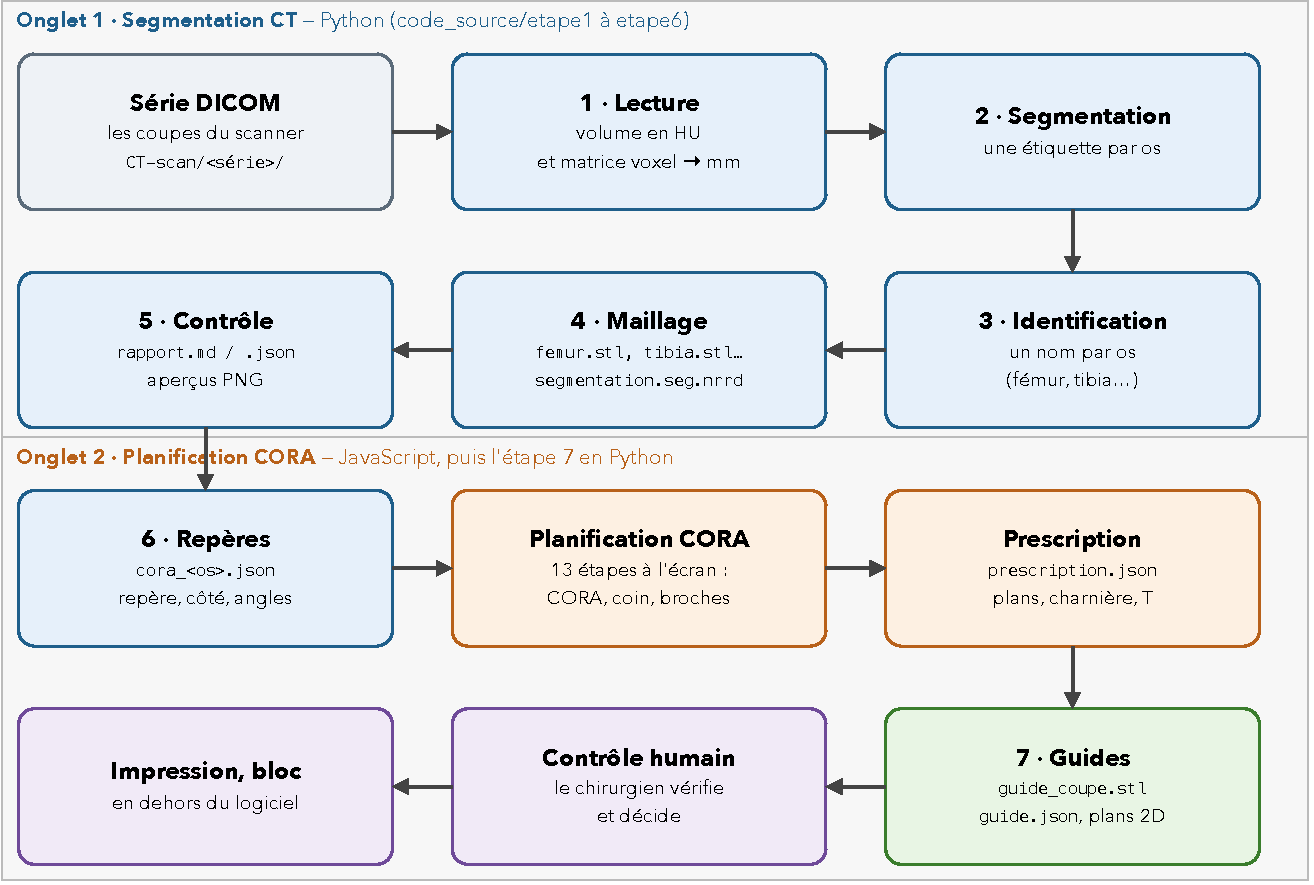
\includegraphics[width=\linewidth]{chaine_complete.pdf}
\caption{La chaîne complète : étapes, programmes et fichiers échangés.}
\label{fig:chaine-complete}
\end{figure}

\begin{table}[htbp]
\centering\small
\caption{Les étapes, leurs entrées, leurs sorties et leur durée (Mac Apple M5, 16~Go de mémoire).}
\label{tab:etapes}
\begin{tabularx}{\linewidth}{L{2.5cm}L{3.1cm}Y L{1.9cm}}
\toprule
\titrecol{Étape} & \titrecol{Fichier du code} & \titrecol{Ce qu'elle produit} & \titrecol{Durée} \\
\midrule
1 · Lecture & \fichier{etape1_lecture_dicom.py} & volume en HU et matrice voxel → millimètres & quelques s \\
2 · Segmentation & \fichier{etape2_segmentation.py} & une étiquette (un numéro) par os & 10 à 40 s \\
3 · Identification & \fichier{etape3_identification.py} & un nom par os ; tête du fémur & quelques s \\
4 · Maillage & \fichier{etape4_maillage.py} & un STL étanche par os, \fichier{segmentation.seg.nrrd} & 10 à 30 s \\
5 · Contrôle & \fichier{etape5_controle.py} & sensibilité au seuil, aperçus, \fichier{rapport.md} et \fichier{.json} & 10 à 40 s \\
6 · Repères & \fichier{etape6_reperes.py} & \fichier{cora_<os>.json} : repère, côté, repères, angles & 1,3 s par os \\
Planification & \fichier{cora/app/cora_simple.js} & \fichier{prescription.json} & instantané \\
7 · Guides & \fichier{etape7_guide.py}, \fichier{dessin_guide.py} & STL à imprimer, \fichier{guide.json}, plans 2D & 11 à 31 s \\
\bottomrule
\end{tabularx}
\end{table}

Les étapes 1 à 6 se lancent ensemble (bouton \ui{Segmenter la série} de l'application, ou
\fichier{lancer_tout.py} en ligne de commande) : de 25~s pour le pied à 2~min pour la série hanche--genou du lévrier.
Tout ce qui est produit pour un scanner va dans \fichier{resultats/<série>/}.

\begin{pourquoi}
\textbf{Pourquoi deux langages ?} Les calculs lourds (images de 200 millions de voxels, maillages, opérations
booléennes) demandent les bibliothèques scientifiques de Python. La planification, elle, doit réagir tout de suite
quand on bouge un curseur et s'afficher en 3D : elle tourne donc dans la page, en JavaScript, avec Three.js pour la
3D. Les deux parties ne partagent que des fichiers (JSON et maillages binaires) : chacune peut être testée seule.
\end{pourquoi}

\section{Les repères}
\label{sec:repere-os}

Trois repères se succèdent.

\textbf{1. Les indices de voxels} $(i, j, k)$ : colonne, ligne et numéro de coupe dans le volume. C'est le repère
du tableau numpy, stocké dans l'ordre $(k, j, i)$.

\textbf{2. Le repère du scanner}, LPS, en millimètres (\cref{sec:scanner}). Une matrice $4 \times 4$, notée
$\mt{A}$, passe des indices aux millimètres (\cref{sec:affine}). Les STL des os sont écrits dans ce repère : ils se
superposent exactement au scanner dans 3D Slicer.

\textbf{3. Le repère de l'os}, propre à chaque fémur ou tibia : $X$ latéral, $Y$ proximal, $Z$ caudal ; origine au
centre de l'articulation distale, au niveau du bout distal de l'os. Il est construit par l'étape 6
(\cref{sec:repere-construction}). Toute la planification et la construction des guides se font dans ce repère.

Le passage du scanner à l'os est une transformation rigide, éventuellement précédée d'un miroir :
\begin{equation}
  \vb{p}_{\text{os}} = \mt{R}\,(\mt{S}\,\vb{p}_{\text{scanner}} - \vb{o}),
  \qquad
  \mt{S} = \begin{cases} \mt{I} & \text{membre droit,} \\ \operatorname{diag}(-1, 1, 1) & \text{membre gauche,} \end{cases}
  \label{eq:repere-os}
\end{equation}
où les lignes de $\mt{R}$ sont les directions $X$, $Y$, $Z$ de l'os (dans le repère du scanner, après miroir) et
$\vb{o}$ son origine. Le logiciel l'écrit sous forme d'une matrice $4 \times 4$ dans \fichier{cora_<os>.json}
(clé \code{scanner_vers_os}). Son déterminant vaut $-1$ quand le membre a été mis en miroir.

\begin{attention}[title={Le miroir retourne les triangles}]
Un miroir change l'orientation de l'espace : un triangle $(a, b, c)$ dont la normale sortait de l'os la ferait
rentrer. Après un miroir, le logiciel inverse donc l'ordre des sommets de chaque triangle, $(a, c, b)$, pour garder
des normales sortantes (fonction \code{miroir_maillage()} de l'étape 6, et \code{maillage_dans_repere()}).
\end{attention}

\section{Les données du projet}
\label{sec:donnees}

\subsection{Les scanners du lévrier}

Le projet dispose de trois scanners d'un lévrier sain, réalisés sur un GE LightSpeed Ultra (120~kV, noyau
« BONEPLUS ») : hanche--genou (728 coupes), genou--cheville (748 coupes) et pied (442 coupes), toutes de 0,625~mm, en
images de $512 \times 512$ pixels de 0,27 à 0,56~mm. Les trois séries sont trois examens distincts. Le fémur complet
est dans la série hanche--genou, le tibia complet dans la série genou--cheville ; les autres fémurs et tibias sont
coupés par le bord du champ et sont refusés pour la méthode CORA (\cref{sec:completude}).

\subsection{L'os fictif}

Pour tester la planification sur un os parfaitement connu, le projet utilise aussi un \textbf{os fictif} : un fémur,
un tibia et une fibula de chien d'environ 30~kg, fabriqués par ordinateur (\fichier{code_source/cora/generate_bones.py}).
Chaque os est une somme lisse de formes simples (sphères, ellipsoïdes, cônes arrondis) décrites par des fonctions de
distance, puis transformée en maillage par marching cubes. Ses repères anatomiques sont connus exactement, et ses
angles sont réglés sur les valeurs publiées (aLPFA 103\degre, aLDFA 97\degre, mMPTA 93,4\degre, mMDTA 96,3\degre,
mCaPTA 63,8\degre, mCrDTA 81,7\degre, antéversion d'environ 31\degre).

\subsection{Les déformités simulées}

Un os sain ne demande pas de correction. Pour tester le logiciel, on lui impose une \textbf{déformité connue}
(\cref{sec:deformite-simulee}) : le segment distal tourne d'un angle choisi autour d'un axe passant par l'apex, avec
éventuellement une torsion. Comme on connaît la réponse, on mesure l'erreur exactement. C'est le niveau 1 de la
validation (\cref{chap:validation}).

\section{Les hypothèses de travail}
\label{sec:hypotheses}

Ce sont les choix faits pour que le projet reste réalisable. Les résultats ne valent que dans ce cadre.
\begin{enumerate}
  \item Un scanner du membre est disponible, avec des coupes de 1~mm ou moins.
  \item La surface d'os trouvée par le logiciel est à moins de 0,5~mm de la vraie surface (vérifié au
  \cref{chap:maillage}).
  \item Chaque os est fait de deux segments droits autour d'\textbf{une seule} zone tordue (un seul apex).
  \item \textbf{Fémur : seulement les déformités distales}, apex entre 62 et 82~\% de la longueur depuis le haut.
  Les déformités du col (coxa vara ou valga, antéversion) se corrigent par une autre ostéotomie et sortent du projet.
  Au tibia, l'apex peut être entre 25 et 85~\%.
  \item La référence est le membre opposé sain, ou à défaut les valeurs normales publiées.
  \item L'os est rigide, et la correction se fait en une fois pendant l'opération.
  \item Les muscles, les ligaments et la plaque ne sont pas modélisés.
  \item Seulement des coupes planes (pas de dôme) ; l'angle et la torsion sont corrigés par un coin suivi d'une
  rotation.
  \item Le chien est adulte par défaut (une option existe pour un chien en croissance).
  \item Les voies d'abord et les marges de sécurité sont des choix raisonnés, à valider avec un chirurgien.
\end{enumerate}

\section{Les bibliothèques utilisées}

Le logiciel n'utilise que des outils gratuits et libres (\cref{tab:bibliotheques}). Ils sont installés une fois par
les lanceurs (\cref{sec:lancer}) ou copiés dans l'application autonome.

\begin{table}[htbp]
\centering\small
\caption{Les bibliothèques et leur rôle.}
\label{tab:bibliotheques}
\begin{tabularx}{\linewidth}{L{3.1cm}YL{2.4cm}}
\toprule
\titrecol{Outil} & \titrecol{Rôle dans le projet} & \titrecol{Licence} \\
\midrule
Python 3.10 et plus & langage des calculs & PSF \\
numpy, scipy \cite{harris2020,virtanen2020} & tableaux, algèbre linéaire, morphologie, arbres k-d & BSD \\
pydicom & lecture des fichiers DICOM & MIT \\
SimpleITK \cite{lowekamp2013} & lissage, ligne de partage des eaux, cartes de distance & Apache 2.0 \\
VTK, pyvista \cite{schroeder2006} & isosurfaces, lissage et décimation de maillages, rendus & BSD, MIT \\
trimesh & maillages : contrôles, coupes, normales & MIT \\
manifold3d \cite{manifold} & opérations booléennes exactes des guides & Apache 2.0 \\
matplotlib & figures, plans 2D & type PSF \\
pywebview & fenêtre native de l'application & BSD \\
Three.js & affichage 3D dans l'interface & MIT \\
PyInstaller & fabrication de l'application autonome & GPL avec exception \\
\bottomrule
\end{tabularx}
\end{table}

\chapter{Étape 1 — Lire le scanner}
\label{chap:lecture}

\begin{chapeau}
Cette étape transforme un dossier de fichiers DICOM en un volume 3D en unités Hounsfield, et calcule la matrice qui
donne la position de chaque voxel en millimètres. Elle fait les mêmes contrôles que le module DICOM de 3D Slicer.
\end{chapeau}

\section{Trouver les séries}

Un dossier apporté par le chirurgien peut contenir plusieurs examens, plusieurs séries, des sous-dossiers, des
fichiers sans extension et des fichiers qui ne sont pas des images (rapports, \fichier{DICOMDIR}). Le logiciel :
\begin{enumerate}
  \item parcourt tout le dossier, sous-dossiers compris, et garde les fichiers dont l'en-tête est DICOM ;
  \item lit seulement l'en-tête (pas les pixels), ce qui est rapide ;
  \item écarte ce qui n'est pas une image en coupe (pas de position ou d'orientation) ;
  \item regroupe les fichiers par série (\code{SeriesInstanceUID}) et donne à chaque série un nom de dossier sûr
  (minuscules, chiffres, tirets), tiré du nom du dossier.
\end{enumerate}

\section{Ranger les coupes dans le bon ordre}

Les fichiers d'une série ne sont pas forcément nommés dans l'ordre, et le champ \code{InstanceNumber}, qui donne
le numéro de l'image, n'est pas fiable. Le logiciel range donc les coupes \textbf{par leur position dans l'espace}. Soient $\vb{r}$ et
$\vb{c}$ les directions des lignes et des colonnes de l'image (les deux triplets de \code{ImageOrientationPatient}).
La normale aux coupes est
\begin{equation}
  \vb{n} = \vb{r} \times \vb{c}.
\end{equation}
La coupe $k$, dont le premier pixel est en $\vb{P}_k$ (\code{ImagePositionPatient}), est à la distance
$d_k = \vb{P}_k \cdot \vb{n}$ le long de cette normale. Trier les coupes, c'est trier les $d_k$.

\section{Contrôler la géométrie}

Avant de lire les pixels, plusieurs contrôles évitent un volume faux :
\begin{itemize}
  \item \textbf{une seule orientation} : les coupes dont l'orientation diffère de la plus fréquente (à $10^{-3}$ près)
  sont écartées. Ce sont en général les images de repérage, comme le topogramme (\cref{sec:topogramme}) ;
  \item \textbf{pas de doublon} : deux coupes à la même position, la seconde est écartée ;
  \item \textbf{espacement régulier} : le pas $\Delta = \operatorname{médiane}(d_{k+1} - d_k)$ ; si un écart s'en
  éloigne de plus de 5~\%, il manque sans doute des coupes ;
  \item \textbf{épaisseur} : au-delà de 1~mm, un avertissement est donné, car la précision des surfaces en souffre.
\end{itemize}

Si l'espacement est irrégulier, le volume est rééchantillonné sur une grille régulière de pas $\Delta$, par
interpolation linéaire entre les deux coupes voisines :
\begin{equation}
  I(d) = (1 - w)\, I_k + w\, I_{k+1},
  \qquad
  w = \frac{d - d_k}{d_{k+1} - d_k},
  \qquad d_k \le d \le d_{k+1}.
\end{equation}

\section{Convertir en unités Hounsfield}

Chaque pixel stocké (\emph{stored value}, SV) devient une valeur en HU par la règle donnée dans l'en-tête :
\begin{equation}
  \tcbhighmath{\mathrm{HU} = \mathrm{SV} \times \texttt{RescaleSlope} + \texttt{RescaleIntercept}.}
\end{equation}
Le volume est gardé en entiers de 16 bits (de $-32\,768$ à $32\,767$), ce qui suffit et divise la mémoire par deux par
rapport à des réels. Si pydicom ne sait pas décoder une image compressée, le logiciel la relit avec SimpleITK.

\section{De l'indice de voxel aux millimètres}
\label{sec:affine}

C'est le calcul le plus important de l'étape : tout ce qui suit (STL, repères, guides) en dépend. Le voxel d'indices
$(i, j, k)$ (colonne, ligne, coupe) est au point
\begin{equation}
  \begin{pmatrix} x \\ y \\ z \\ 1 \end{pmatrix}
  = \underbrace{\begin{pmatrix}
    \Delta_c\, r_x & \Delta_r\, c_x & \delta_x & P_{0,x} \\
    \Delta_c\, r_y & \Delta_r\, c_y & \delta_y & P_{0,y} \\
    \Delta_c\, r_z & \Delta_r\, c_z & \delta_z & P_{0,z} \\
    0 & 0 & 0 & 1
  \end{pmatrix}}_{\mt{A}}
  \begin{pmatrix} i \\ j \\ k \\ 1 \end{pmatrix},
  \qquad
  \boldsymbol{\delta} = \frac{\vb{P}_{N-1} - \vb{P}_0}{N - 1},
  \label{eq:affine}
\end{equation}
où $\Delta_c$ est l'écart entre deux colonnes et $\Delta_r$ l'écart entre deux lignes (\code{PixelSpacing} donne
$[\Delta_r, \Delta_c]$, dans cet ordre), $\vb{P}_0$ la position du premier voxel et $\boldsymbol{\delta}$ le pas
réel d'une coupe à la suivante, calculé avec la première et la dernière coupe.

\begin{pourquoi}
On pourrait prendre $\boldsymbol{\delta} = \Delta\,\vb{n}$. Mais si le statif du scanner était incliné
(\emph{gantry tilt}), les coupes glissent les unes par rapport aux autres et le pas n'est pas parallèle à la normale.
Avec $\boldsymbol{\delta}$ mesuré sur les positions, la matrice reste exacte. L'inclinaison est
$\arccos\bigl(\abs{\boldsymbol{\delta}\cdot\vb{n}} / \norm{\boldsymbol{\delta}}\bigr)$ ; au-delà de 0,5\degre, le
logiciel le signale.
\end{pourquoi}

L'opération inverse, des millimètres aux indices, résout le système linéaire :
$(i, j, k)^{\mathsf T} = \mt{A}_{3\times3}^{-1}\,(\vb{p} - \vb{P}_0)$. Les indices obtenus peuvent être
fractionnaires : on interpole alors entre les voxels.

\begin{exemple}
Série genou--cheville du lévrier : 748 coupes de $512 \times 512$ pixels, voxel de
$0{,}625 \times 0{,}56 \times 0{,}56$~mm, soit un volume de $467 \times 287 \times 287$~mm et
196 millions de voxels (392~Mo en entiers de 16 bits). Statif non incliné.
\end{exemple}

\begin{danslecode}
\fichier{code_source/etape1_lecture_dicom.py} :
\code{inventaire()} trouve et regroupe les séries ; \code{charger()} trie, contrôle, lit, convertit en HU et
construit la matrice $\mt{A}$ (classe \code{Volume}, avec \code{vers_lps()} et \code{vers_indices()}) ;
\code{lire_pixels()} applique \code{RescaleSlope} et \code{RescaleIntercept}. Réglages dans
\fichier{parametres.py} : \code{EPAISSEUR_MAX_MM}, \code{TOLERANCE_ESPACEMENT}, \code{TOLERANCE_ORIENTATION}.
\end{danslecode}

\begin{attention}[title={Données personnelles}]
L'en-tête DICOM contient souvent le nom de l'animal, parfois celui du propriétaire, et un identifiant. L'inventaire
les lit, et le rapport de l'étape 5 les recopie (\cref{sec:securite}). Il vaut mieux rendre les scanners anonymes avant
de les importer.
\end{attention}

\chapter{Étape 2 — Séparer les os}
\label{chap:segmentation}

\begin{chapeau}
La segmentation décide, pour chaque voxel, à quel os il appartient. Le résultat est un tableau d'étiquettes : 0 pour
« pas d'os », puis un numéro par os. Les noms (fémur, tibia\ldots) viennent à l'étape 3.
\end{chapeau}

\section{La difficulté : les os se touchent}

Un simple seuil ne suffit pas. Au seuil de l'os (226~HU), tout le membre forme un seul bloc : dans chaque articulation,
quelques voxels de volume partiel relient les deux os (\cref{fig:segmentation-principe}, image 2). Monter le seuil
sépare les os, mais efface aussi l'os spongieux et les corticales fines. L'idée de la méthode est de se servir des
deux seuils : un seuil \emph{haut} pour trouver une graine par os, puis le seuil \emph{bas} pour reconstruire chaque os
en entier.

\fig{segmentation_principe.png}{La segmentation sur une vraie coupe du genou du lévrier : (1) l'image du scanner ;
(2) au seuil de 226~HU, les os se touchent ; (3) avec un seuil plus haut, il reste un noyau par os ; (4) chaque os
grandit jusqu'à l'articulation. La figure est en 2D ; le logiciel travaille en 3D.}{fig:segmentation-principe}

\section{Préparer le volume}

\subsection{Recadrer}

Le volume complet contient la table du scanner, l'air et les tissus mous. Le logiciel cherche d'abord la boîte qui
contient les os denses ($\geq 500$~HU, morceaux d'au moins 30~mm³), en travaillant sur un volume deux fois plus petit
dans chaque direction, puis l'agrandit de 6~mm. Toute la suite se fait dans cette boîte : la mémoire nécessaire est
divisée par cinq environ.

\subsection{Lisser}

Le bruit (environ 49~HU) crée des voxels isolés au-dessus du seuil. On applique un flou gaussien de
$\sigma = 0{,}35$~mm, c'est-à-dire on remplace chaque valeur par une moyenne pondérée de ses voisines :
\begin{equation}
  I_\sigma(\vb{x}) = \int I(\vb{y})\, \frac{1}{(2\pi\sigma^2)^{3/2}} \exp\!\left(-\frac{\norm{\vb{x}-\vb{y}}^2}{2\sigma^2}\right) \dd\vb{y}.
\end{equation}
Le $\sigma$ est donné en millimètres : le flou est le même dans les trois directions, même si les voxels ne sont pas
cubiques. Ce lissage divise le bruit environ par deux sans effacer les interlignes articulaires (1~mm et plus).

\subsection{Le masque osseux}

Le masque osseux est l'ensemble $M = \{\vb{x} : I_\sigma(\vb{x}) \geq 226~\mathrm{HU}\}$. Ce seuil est celui que
propose le logiciel Mimics pour l'os au scanner ; le document de cadrage du projet donnait 200 à 300~HU.

\section{Une graine par os : le seuil qui monte}
\label{sec:graines}

On monte le seuil par paliers de 100~HU, de 500 à 1500~HU. À chaque palier, on regarde les \emph{composantes
connexes} : les groupes de voxels au-dessus du seuil qui se touchent (par une face, une arête ou un coin : 26
voisins). Quand un bloc se coupe en morceaux, c'est en général parce qu'une articulation, moins dense que l'os, vient
de céder.

Un bloc $B$ est coupé au palier $T$ quand, parmi les composantes de $B \cap \{I_\sigma \geq T\}$, au moins deux
\begin{itemize}
  \item sont assez grosses : au moins 300~mm³ ;
  \item et \textbf{persistent} : elles gardent au moins 50~mm³ au palier $T + 200$~HU.
\end{itemize}
Chaque morceau retenu est alors examiné à son tour aux paliers suivants. C'est un arbre : le membre se coupe en
segments, qui se recoupent en os. Les feuilles de l'arbre sont les graines.

\begin{pourquoi}
\textbf{Pourquoi la persistance ?} Un vrai os a une corticale dense, qui reste visible quand le seuil monte encore. Un
fragment d'os spongieux, lui, disparaît vite : sans ce critère, l'épiphyse spongieuse d'un os pourrait devenir une
graine à part.
\end{pourquoi}

\begin{exemple}
Sur le lévrier, le genou se sépare dès 600~HU, la hanche vers 900~HU (la tête du fémur reste collée au bassin plus
longtemps), et les os du tarse vers 1200 à 1400~HU.
\end{exemple}

\section{La croissance de région compétitive}
\label{sec:croissance}

Les graines grandissent ensuite toutes en même temps dans le masque osseux $M$. On utilise pour cela la
\textbf{ligne de partage des eaux à partir de marqueurs} \cite{meyer1994}. Imaginons l'image comme un relief :
\begin{equation}
  R(\vb{x}) = \clamp\bigl(3000 - I_\sigma(\vb{x}),\ 0,\ 4500\bigr).
\end{equation}
Les zones denses sont des vallées, les interlignes (peu denses) des crêtes. Chaque graine est une source d'eau. L'eau
monte : à chaque instant, on inonde le voxel le plus bas du relief (le plus dense) parmi ceux qui touchent une zone
déjà inondée, et il prend la couleur de cette zone. Deux os qui grandissent se rencontrent donc là où la densité est
la plus faible entre eux : dans l'interligne.

\noindent\begin{minipage}{\linewidth}
\begin{lstlisting}[language=Python, title={Principe (pseudo-code)}]
file = voisins des graines, classés par relief croissant
tant que la file n'est pas vide :
    x = le voxel de plus petit relief de la file
    etiquette[x] = etiquette du voisin déjà inondé qui l'a atteint
    ajouter à la file les voisins de x qui sont dans le masque et pas encore inondés
\end{lstlisting}
\end{minipage}

Le « fond » (tout ce qui est hors du masque) est aussi une source : il empêche les os de déborder du masque. Le calcul
est fait par la fonction \code{MorphologicalWatershedFromMarkers} de SimpleITK \cite{lowekamp2013}.

\section{Recoller les morceaux d'un même os}
\label{sec:cstar}

À haut seuil, une épiphyse se détache parfois de la diaphyse, parce que la corticale de la métaphyse est fine : un
même os donne alors deux graines. Mais ces deux morceaux se touchent sur \emph{toute la section} de l'os, alors que
deux os voisins ne se touchent que sur une petite surface d'articulation. On mesure cela par un nombre sans
dimension :
\begin{equation}
  \tcbhighmath{c^* = \frac{A_{\text{contact}}}{V_{\min}^{2/3}},}
  \label{eq:cstar}
\end{equation}
où $A_{\text{contact}}$ est la surface de contact entre les deux morceaux (le nombre de faces de voxels qu'ils
partagent, multiplié par l'aire d'une face) et $V_{\min}$ le volume du plus petit des deux.

\begin{pourquoi}
\textbf{Pourquoi la puissance 2/3 ?} Pour un objet de taille $L$, le volume varie comme $L^3$ et une section comme
$L^2$, donc comme $V^{2/3}$. Le rapport $c^*$ ne dépend donc pas de la taille du chien : une coupure à travers un os
donne toujours $c^*$ de l'ordre de quelques unités, quelle que soit la taille de l'os.
\end{pourquoi}

\fig{critere_contact.pdf}{Le critère $c^*$ mesuré sur le lévrier : les vraies articulations restent sous 2,1 ; un
même os coupé en deux donne environ 5. Le seuil de recollage est fixé à 3.}{fig:critere-contact}

Le recollage est glouton : on fusionne d'abord la paire de plus grand $c^*$, puis on met à jour la table des contacts
sans tout recalculer, grâce à la relation exacte
$A_{\text{contact}}(A \cup B, C) = A_{\text{contact}}(A, C) + A_{\text{contact}}(B, C)$. On recommence tant qu'une
paire dépasse le seuil. Enfin, les segments de moins de 50~mm³ sont rattachés au voisin avec lequel ils ont le plus
grand contact (ou supprimés s'ils sont isolés), et les étiquettes sont renumérotées par volume décroissant.

\section{Résultat}

\fig[0.82]{segmentation_resultat.png}{Les os segmentés automatiquement dans le scanner hanche--genou du
lévrier.}{fig:segmentation-resultat}

\begin{exemple}
Série hanche--genou (728 coupes) : lissage 7~s, graines 10,5~s, croissance 15~s, recollage 5~s. Le fémur fait
100,3~cm³. Pour les séries genou--cheville et pied, la segmentation prend 7 à 8~s (après recadrage).
\end{exemple}

\begin{danslecode}
\fichier{code_source/etape2_segmentation.py} : \code{recadrage()}, \code{lisser()},
\code{graines_automatiques()} (l'arbre des seuils, fonction interne \code{couper()}), \code{croissance()} (ligne de
partage des eaux), \code{contacts()} (surfaces de contact), \code{fusionner_surdecoupages()} (critère $c^*$),
\code{nettoyer()}, et \code{segmenter()} qui enchaîne le tout. Deux outils servent à l'étape 3 :
\code{recroissance()} (nouvelle croissance dans une zone, avec des graines imposées) et \code{raffiner()} (graines plus
fines dans un seul segment). Réglages : \code{SEUIL_OS_HU}, \code{SIGMA_LISSAGE_MM}, \code{SEUIL_GRAINE_*},
\code{PERSISTANCE_HU}, \code{RAPPORT_CONTACT_FUSION}\ldots{} (\cref{ann:parametres}).
\end{danslecode}

\chapter{Étape 3 — Donner un nom à chaque os}
\label{chap:identification}

\begin{chapeau}
Après la segmentation, chaque os a un numéro. Cette étape lui donne un nom (fémur, tibia, fibula, rotule\ldots) avec
des règles anatomiques simples, et corrige trois erreurs typiques de la segmentation : la tête du fémur collée au
bassin, la fibula collée au tibia et les fabelles collées au fémur.
\end{chapeau}

\section{Décrire chaque segment}

Pour chaque segment, le logiciel calcule des descripteurs : son volume, sa densité moyenne, ses contacts avec ses
voisins, s'il touche le bord du champ du scanner, et surtout sa \textbf{forme} par une analyse en composantes
principales.

\subsection{L'analyse en composantes principales}
\label{sec:acp}

Soient $\vb{p}_1, \ldots, \vb{p}_N$ les centres des voxels du segment (en mm) et $\vb{c}$ leur moyenne. On forme la
matrice $\mt{X}$ ($N \times 3$) des points centrés, de lignes $\vb{p}_i - \vb{c}$, et on la décompose en valeurs
singulières :
\begin{equation}
  \mt{X} = \mt{U}\,\boldsymbol{\Sigma}\,\mt{V}^{\mathsf T}.
\end{equation}
Les colonnes $\vb{v}_1, \vb{v}_2, \vb{v}_3$ de $\mt{V}$ sont les directions principales : $\vb{v}_1$ est la
direction dans laquelle l'objet est le plus étendu. Ce sont aussi les vecteurs propres de la matrice de covariance
$\mt{X}^{\mathsf T}\mt{X}/N$. On projette les points sur chaque direction, $t_{ik} = (\vb{p}_i - \vb{c})\cdot\vb{v}_k$,
et on prend comme longueur $L_k$ l'écart entre le 1\textsuperscript{er} et le 99\textsuperscript{e} centile (ce qui
ignore quelques voxels isolés). L'\textbf{allongement} est $L_1 / L_2$ : un os long a un allongement supérieur à 3,
un os compact (rotule, os du tarse) inférieur à 3,5.

\subsection{Densité et objets non osseux}

Un fantôme de calibration ou une tige posée sur la table peut ressembler à un os. On le reconnaît à son intérieur :
mesuré sur les voxels intérieurs (le segment érodé de deux voxels, pour ignorer les bords flous), il est homogène
(coefficient de variation des HU inférieur à 0,2), presque sans os spongieux (moins de 8~\% de voxels sous 600~HU) et
\emph{sans cavité} à remplir. Un os, lui, a toujours un canal médullaire ou de l'os spongieux : remplir le fémur du
lévrier augmente son volume de 29~\%.

\section{Les règles, de la plus sûre à la moins sûre}

\begin{table}[htbp]
\centering\small
\caption{Les règles d'identification, dans l'ordre où elles sont appliquées.}
\label{tab:regles-os}
\begin{tabularx}{\linewidth}{rL{2.6cm}Y}
\toprule
& \titrecol{Os} & \titrecol{Règle} \\
\midrule
1 & objet non osseux & intérieur homogène et dense, et aucune cavité à remplir \\
2 & tibia, fibula & un os long fin (allongement $\geq 6$), parallèle (moins de 20\degre) et qui recouvre au moins la moitié de la longueur touche un gros os long \\
3 & fémur, bassin & une sphère (la tête du fémur) est trouvée au contact d'un gros voisin (\cref{sec:tete}) \\
4 & genou & le gros os au contact de l'extrémité la plus large du tibia (le plateau) est le fémur, et inversement \\
5 & fibula collée & sur des tranches du tibia, une petite tache séparée est suivie sur au moins 15~\% de la longueur (\cref{sec:fibula}) \\
6 & métatarses & au moins trois os longs, fins, parallèles et voisins \\
7 & tibia (pied seul) & le gros os au-dessus du tarse, si aucune autre règle ne l'a trouvé \\
8 & talus, calcanéus, tarse & os compacts reliés au bout du tibia : le talus a le plus grand contact avec le tibia, le calcanéus est le plus long \\
9 & phalanges & au-delà des métatarses \\
10 & rotule, fabelles & petits os compacts au contact du fémur ; le plus gros est la rotule \\
11 & bassin & gros os reliés à l'acétabulum par de larges contacts \\
12 & points de l'utilisateur & renommer un segment, ou le séparer s'il contient des points de plusieurs noms \\
13 & côtés & deux fémurs ou deux tibias : suffixe \code{_gauche} ou \code{_droit} selon $x$ (LPS) \\
\bottomrule
\end{tabularx}
\end{table}

Chaque nom est accompagné de sa \textbf{raison}, écrite en clair dans le rapport, par exemple « os long longé par un os
long fin et parallèle (fibula, segment 7) ». L'utilisateur peut ainsi vérifier pourquoi le logiciel a décidé.

\section{La tête du fémur}
\label{sec:tete}

La hanche est l'articulation la plus serrée : sur ce scanner, la tête du fémur touche l'acétabulum jusqu'à 1100~HU,
alors qu'elle se détache déjà du col vers 900~HU. Aucun seuil ne la rend au fémur. Mais l'interligne reste visible :
c'est une ligne sombre de 1 à 2 voxels, entre deux zones denses.

\subsection{Révéler l'interligne}

Une \emph{fermeture morphologique} en niveaux de gris, par une boule de rayon $\rho = 1$~mm, remplace chaque valeur par
le minimum des maxima voisins : elle « bouche » les vallées étroites. La différence entre l'image fermée et l'image
de départ, appelée \emph{chapeau haut-de-forme noir} (\emph{black top-hat}),
\begin{equation}
  V(\vb{x}) = (I \bullet B_\rho)(\vb{x}) - I(\vb{x}),
\end{equation}
est grande exactement dans les vallées plus étroites que la boule. On garde les voxels où $V > 250$~HU, où l'image
dépasse 150~HU (pour écarter les cloisons de graisse entre les muscles), près du contact fémur--bassin.

\subsection{Ajuster une sphère par RANSAC}

Ces points dessinent une portion de sphère, mêlée à d'autres vallées. On cherche la sphère par la méthode
\textbf{RANSAC} \cite{fischler1981} (\cref{fig:ransac}) :
\begin{enumerate}
  \item tirer 4 points au hasard et calculer la sphère qui passe par eux ;
  \item garder cette sphère seulement si son rayon est plausible (4 à 20~mm, d'un chien miniature à un chien géant) ;
  \item compter les points à moins de 0,6~mm de la sphère (les \emph{inliers}) ;
  \item recommencer 4000 fois et garder la sphère qui a le plus d'inliers ;
  \item l'affiner par moindres carrés sur ses inliers (trois fois).
\end{enumerate}

\fig[0.9]{ransac_cercle.pdf}{Le principe de RANSAC, montré en 2D avec un cercle : un essai au hasard est soutenu par
peu de points ; le meilleur essai, affiné, retrouve la courbe malgré les points parasites.}{fig:ransac}

\textbf{La sphère par les moindres carrés.} Un point $\vb{p}$ est sur la sphère de centre $\vb{c}$ et de rayon $r$
si $\norm{\vb{p} - \vb{c}}^2 = r^2$. En développant :
\begin{equation}
  \tcbhighmath{\norm{\vb{p}}^2 = 2\,\vb{c}\cdot\vb{p} + s, \qquad s = r^2 - \norm{\vb{c}}^2.}
  \label{eq:sphere}
\end{equation}
Cette équation est \emph{linéaire} en $(\vb{c}, s)$. Avec 4 points, c'est un système $4 \times 4$ ; avec $N$ points,
on résout au sens des moindres carrés le système $[\,2\vb{p}_i^{\mathsf T}\ \ 1\,]\,(\vb{c}, s)^{\mathsf T} =
\norm{\vb{p}_i}^2$, puis $r = \sqrt{s + \norm{\vb{c}}^2}$.

\begin{exemple}[title={Exemple chiffré : combien d'essais ?}]
Si une fraction $w$ des points candidats est sur la sphère, la probabilité qu'un tirage de 4 points ne contienne que
des bons points est $w^4$. Pour trouver au moins un bon tirage avec une probabilité $P$, il faut
$n = \ln(1 - P) / \ln(1 - w^4)$ essais. Avec $w = 0{,}3$ et $P = 0{,}999$ : $n \approx 850$. Les 4000 essais du
logiciel laissent une large marge.
\end{exemple}

\subsection{Vérifier la sphère, puis séparer}

Une vraie tête de fémur est couverte de points dans beaucoup de directions. On mesure la \textbf{couverture} : la
fraction de 200 directions réparties régulièrement sur la sphère (directions de Fibonacci,
$\phi_g = \arccos(1 - 2g/200)$, $\lambda_g = \pi(1 + \sqrt5)\,g$) qui ont un inlier à moins de 25\degre. La sphère est
acceptée si elle a au moins 150 inliers et une couverture d'au moins 40~\%.

La zone fémur + bassin est alors redistribuée par une nouvelle croissance de région : graine « fémur » à l'intérieur de
la sphère (rayon $- 1$~mm), graine « bassin » au-delà (rayon $+ 1$~mm). La frontière tombe dans l'interligne. Le centre
et le rayon sont écrits dans \fichier{reperes_auto.mrk.json}, au format Markups de 3D Slicer.

\begin{exemple}
Lévrier : sphère de rayon 12,6~mm, soutenue par 2055 points, couverture 68~\%.
\end{exemple}

\section{La fibula collée au tibia}
\label{sec:fibula}

Aux deux bouts de la jambe, la fibula touche le tibia ; au milieu, elle en est séparée. Le logiciel coupe le segment
« tibia » en tranches de 2~mm perpendiculaires à son axe principal. Sur chaque tranche remplie, il cherche une petite
tache séparée : au moins 3~mm² et moins de 20~\% de l'aire du tibia (sur le lévrier : 17~mm² contre 300~mm²). Il garde
la plus longue suite de tranches où la tache existe et se déplace de moins de 3~mm d'une tranche à l'autre. Si cette
suite couvre au moins 15~\% de la longueur (45~\% sur le lévrier), les taches servent de graine « fibula », les grandes
de graine « tibia », et une croissance de région redistribue le segment. Un garde-fou annule la séparation si la
fibula obtenue est invraisemblable (moins de 2~\% ou plus de 25~\% du volume du tibia, ou moins de 40~\% de sa longueur).

\section{Les fabelles et les autres corrections}

\begin{itemize}
  \item \textbf{Fabelles.} Trop petites pour avoir leur graine, elles restent collées au fémur. Le fémur est
  re-segmenté avec des graines trois fois plus fines ; seuls les petits morceaux compacts et peu en contact
  ($c^* < 1{,}5$, moins de 5~\% du fémur) deviennent des fabelles. Sur le lévrier : 0,43~cm³.
  \item \textbf{Talus soudé à un rayon du pied.} Un segment allongé qui touche la jambe n'est pas un métatarse pur (un
  métatarse ne touche jamais le tibia) : il est re-découpé finement.
  \item \textbf{Morceaux détachés.} Un os nommé doit être d'un seul tenant : un morceau détaché est rendu à l'os dont
  il a été coupé s'il le touche sur une section entière ($c^* \geq 3$), sinon il devient un segment à part.
\end{itemize}

\section{Les corrections de l'utilisateur}

Dans l'onglet \ui{Segmentation CT}, l'utilisateur peut \ui{Renommer} un segment ou le \ui{Séparer} en cliquant des
points sur les coupes. Chaque point porte un nom ; il est enregistré dans \fichier{resultats/<série>/graines.json} et
réappliqué à chaque calcul. Si un segment contient des points de plusieurs noms, une croissance de région part de
boules de 2,5~mm autour des points et redistribue le segment, une étiquette par nom.

\begin{danslecode}
\fichier{code_source/etape3_identification.py} : \code{decrire()} (descripteurs, ACP), \code{identifier()} (les
13 règles, dans l'ordre), \code{tete_femorale()} et \code{ajuster_sphere()} (chapeau haut-de-forme, RANSAC, couverture),
\code{separer_fibula()}, \code{points_par_etiquette()} et \code{separer_par_points()} (points de l'utilisateur),
\code{nettoyer_morceaux()}, \code{nommer_cotes()}.
\end{danslecode}

\chapter{Étapes 4 et 5 — Fabriquer les surfaces et les contrôler}
\label{chap:maillage}

\begin{chapeau}
L'étape 4 transforme chaque os segmenté en une surface 3D fermée, un fichier STL. L'étape 5 mesure la sensibilité du
résultat au seuil choisi et écrit les rapports.
\end{chapeau}

\section{Remplir l'os}

Le STL doit décrire la surface extérieure de l'os, pas le canal médullaire. On remplit donc chaque os :
\begin{enumerate}
  \item une \textbf{fermeture morphologique} de rayon 1~mm (une dilatation suivie d'une érosion) bouche les petits
  pores de la corticale ;
  \item si l'os sort du champ du scanner, sa section au bord est d'abord fermée par un \textbf{couvercle} (la section
  remplie en 2D) : sinon le canal resterait ouvert et ne se remplirait pas ;
  \item un \textbf{remplissage des trous} en 3D remplit tout ce qui n'est pas relié à l'extérieur : canal et os
  spongieux.
\end{enumerate}

\section{Extraire la surface}

\subsection{Marching cubes}

Le masque rempli vaut 1 dans l'os et 0 dehors. On le floute légèrement ($\sigma = 0{,}3$~mm) pour obtenir un champ
$g$ qui passe en douceur de 1 à 0, puis on extrait la surface $g = 0{,}5$ par l'algorithme des \emph{marching cubes}
\cite{lorensen1987}, dans sa version rapide \emph{Flying Edges} \cite{schroeder2015}. Le principe : on parcourt les
petits cubes formés par 8 voxels voisins. Pour chaque cube, on regarde quels coins sont au-dessus de 0,5 ; parmi les
256 cas possibles, une table donne les triangles à placer dans le cube. Le sommet d'un triangle posé sur l'arête qui
relie deux coins $a$ et $b$ est placé par interpolation linéaire, au point
\begin{equation}
  \vb{x} = \vb{x}_a + t\,(\vb{x}_b - \vb{x}_a), \qquad t = \frac{0{,}5 - g_a}{g_b - g_a}.
\end{equation}
Le léger flou supprime l'effet d'escalier des voxels. Les sommets, calculés en indices de voxels, passent ensuite en
millimètres par la matrice $\mt{A}$ (\cref{eq:affine}).

\subsection{Lisser sans rétrécir}

Un lissage simple, qui rapproche chaque sommet de la moyenne de ses voisins, fait rétrécir le maillage. On utilise un
lissage « à fenêtre sinc » \cite{taubin1995} (20 itérations, bande passante 0,05) : c'est un filtre passe-bas sur la
position des sommets, qui enlève les petites bosses sans changer la taille de l'objet. C'est aussi le choix de 3D
Slicer.

\subsection{Alléger}

Au-delà de 150\,000 triangles (environ 7~Mo de STL), le maillage est simplifié par la méthode des \emph{quadriques}
\cite{garland1997}. Chaque sommet accumule une matrice $\mt{Q} = \sum_{p} \vb{p}\vb{p}^{\mathsf T}$, où
$\vb{p} = (a, b, c, d)$ décrit le plan $ax + by + cz + d = 0$ de chaque triangle voisin. L'erreur
$\vb{x}^{\mathsf T}\mt{Q}\,\vb{x}$ (en coordonnées homogènes) est la somme des carrés des distances de $\vb{x}$ à ces
plans. On fusionne en priorité les sommets dont la fusion coûte le moins. La simplification n'est gardée que si le
maillage reste étanche, et elle ne retire jamais plus de 75~\% des triangles.

\section{Placer la surface au vrai bord}
\label{sec:demi-hauteur}

\subsection{Le biais d'un seuil bas}

Le scanner floute les bords (\cref{sec:scanner}). Modélisons un bord d'os par une marche floutée : du côté de l'os
(position $s < 0$ le long de la normale) l'intensité vaut $C$ (corticale, environ 1300~HU), dehors elle vaut $B$
(tissus mous, environ 40~HU), et entre les deux
\begin{equation}
  I(s) = B + (C - B)\,\Phi\!\left(-\frac{s}{\sigma}\right),
  \label{eq:bord}
\end{equation}
où $\Phi$ est la fonction de répartition de la loi normale et $\sigma$ l'écart-type du flou. Le vrai bord est en
$s = 0$, là où l'intensité vaut la moitié entre $B$ et $C$. Un seuil $T$ place la surface là où $I(s) = T$, donc en
\begin{equation}
  \tcbhighmath{s_T = -\sigma\,\Phi^{-1}\!\left(\frac{T - B}{C - B}\right).}
  \label{eq:biais}
\end{equation}

\fig{profil_bord.pdf}{Un seuil bas (226~HU) place la surface trop à l'extérieur d'environ un écart-type du flou ; la
demi-hauteur retrouve le vrai bord.}{fig:profil-bord}

\begin{exemple}
Fantôme du test \fichier{test_chaine.py} : flou du scanner $\sigma_{\text{PSF}} = 0{,}5$~mm et lissage du logiciel
$0{,}35$~mm, soit $\sigma = \sqrt{0{,}5^2 + 0{,}35^2} = 0{,}61$~mm. Avec $T = 226$, $B = 40$ et $C = 1300$~HU :
$(T - B)/(C - B) = 0{,}148$, $\Phi^{-1}(0{,}148) = -1{,}05$, donc $s_T = +0{,}64$~mm. Le test mesure $+0{,}60$~mm : la
surface au seuil est trop grande de 0,6~mm, plus que la tolérance de 0,5~mm du projet.
\end{exemple}

\subsection{L'affinage à demi-hauteur}

Pour supprimer ce biais, chaque sommet est déplacé le long de sa normale jusqu'au point où l'intensité vaut la moitié
entre le pic de la corticale et le fond :
\begin{enumerate}
  \item on lit le profil d'intensité le long de la normale, de 2,5~mm à l'intérieur à 2~mm à l'extérieur, tous les
  0,1~mm (interpolation trilinéaire dans l'image) ;
  \item le \emph{pic} est le maximum du côté intérieur, le \emph{fond} le minimum après le pic ;
  \item le nouveau bord est le premier point, après le pic, où le profil passe sous $(\text{pic} + \text{fond})/2$
  (interpolation linéaire entre deux échantillons) ;
  \item le déplacement est ignoré si le contraste est faible (moins de 300~HU) ou s'il dépasse 1,5~mm (articulation
  serrée, profil douteux) ;
  \item les déplacements sont lissés sur le maillage (cinq passes de moyenne avec les voisins), pour ne pas créer de
  bruit d'un sommet à l'autre.
\end{enumerate}

\begin{exemple}
Sur le fantôme, l'écart passe de $+0{,}60$ à $+0{,}16$~mm ; le reste vient de la corticale très fine du fantôme
(1,5~mm), dont le pic est atténué par le flou. Sur le lévrier, les sommets reculent en moyenne de 0,21 à 0,32~mm
vers l'intérieur selon l'os.
\end{exemple}

\section{Vérifier que la surface est fermée}

Un fichier à imprimer doit décrire un solide fermé. Le logiciel vérifie :
\begin{itemize}
  \item l'\textbf{étanchéité} : chaque arête est partagée par exactement deux triangles ;
  \item l'\textbf{orientation} : les triangles voisins sont parcourus dans le même sens, et les normales sortent de
  l'os. Le volume, calculé par $V = \tfrac16 \sum_{\text{triangles}} \vb{a}\cdot(\vb{b}\times\vb{c})$, doit être
  positif ; sinon on retourne tous les triangles ;
  \item la \textbf{caractéristique d'Euler} $\chi = S - A + F$ (sommets, arêtes, faces) vaut 2 pour une surface fermée
  sans trou, comme une sphère. Un os seul doit donner $\chi = 2$ ; un groupe de $n$ os sans trou donne $2n$.
\end{itemize}

Les fichiers sont écrits au format \textbf{STL binaire} : 80 octets d'en-tête, le nombre de triangles, puis
50 octets par triangle (sa normale, ses trois sommets en réels de 4 octets et 2 octets libres). Le logiciel écrit aussi
\fichier{segmentation.seg.nrrd}, qui contient toutes les étiquettes avec leurs noms et leurs couleurs et s'ouvre dans
3D Slicer par-dessus la série DICOM, pour vérifier ou retoucher.

Enfin, l'étape 4 note les \textbf{bords du champ} touchés par chaque os (un plan et sa normale) : l'étape 6 s'en sert
pour savoir si une extrémité articulaire manque (\cref{sec:completude}).

\section{Étape 5 — La sensibilité au seuil}
\label{sec:sensibilite}

Le document de cadrage demandait de vérifier que le résultat ne dépend pas trop du seuil choisi (« variation du seuil
de ± 50~HU et mesure de l'impact »). Pour chaque os principal, le logiciel :
\begin{enumerate}
  \item re-segmente l'os à 176 puis à 276~HU, dans la même zone (l'os dilaté de 3~mm, sans les autres os) ;
  \item le remplit de la même façon et en extrait la surface ;
  \item mesure la distance de chaque sommet de cette nouvelle surface à la surface de référence.
\end{enumerate}
La distance est calculée avec une précision inférieure au voxel. Si $g$ est le masque de référence flouté (celui du
STL) et $\vb{p}$ un point proche de la surface $g = 0{,}5$, un développement au premier ordre donne
\begin{equation}
  g(\vb{p}) \approx 0{,}5 - d\,\norm{\nabla g(\vb{p})}
  \quad\Longrightarrow\quad
  d \approx \frac{0{,}5 - g(\vb{p})}{\norm{\nabla g(\vb{p})}},
\end{equation}
avec $d > 0$ quand la nouvelle surface est à l'extérieur. Loin de la surface ($g$ proche de 0 ou de 1), on prend une
carte de distance exacte au voxel près (transformée de Maurer \cite{maurer2003}).

\begin{table}[htbp]
\centering\small
\caption{Sensibilité au seuil sur le lévrier : écart moyen (en valeur absolue) entre la surface à 226~HU et celle à
176~HU, et 95\textsuperscript{e} centile de l'écart avec la surface à 276~HU.}
\label{tab:sensibilite}
\begin{tabular}{lrr}
\toprule
\titrecol{Os (série)} & \titrecol{écart moyen, 176 HU (mm)} & \titrecol{95\textsuperscript{e} centile, 276 HU (mm)} \\
\midrule
fémur (hanche--genou) & 0,10 & 0,38 \\
tibia (genou--cheville) & 0,11 & 0,40 \\
fibula (genou--cheville) & 0,17 & 0,40 \\
rotule (genou--cheville) & 0,20 & 0,46 \\
talus (genou--cheville) & 0,21 & 0,39 \\
\bottomrule
\end{tabular}
\end{table}

Les grands os bougent en moyenne d'un dixième de millimètre ; 95~\% des points restent à moins de 0,5~mm. Les petits
os fins (fibula, rotule, talus) sont un peu plus sensibles.

\section{Les rapports}

Pour chaque série, l'étape 5 écrit dans \fichier{resultats/<série>/} :
\begin{itemize}
  \item \fichier{rapport.md} (lisible) et \fichier{rapport.json} (toutes les valeurs) : la série, les os exportés
  (volume, triangles, étanchéité, Euler, affinage, sensibilité), l'identification avec ses raisons, les avertissements ;
  \item \fichier{apercu_3d.png} et \fichier{apercu_coupes.png}, pour un contrôle visuel rapide ;
  \item \fichier{reperes_auto.mrk.json} : la tête du fémur, au format de 3D Slicer.
\end{itemize}

\begin{danslecode}
\fichier{code_source/etape4_maillage.py} : \code{remplir()}, \code{mailler()} (flou, Flying Edges, lissage,
décimation, normales), \code{affiner_demi_hauteur()}, \code{controle()} (étanchéité, Euler, volume),
\code{bords_touches()}, \code{ecrire_stl()}, \code{ecrire_seg_nrrd()} et \code{lire_seg_nrrd()}, \code{exporter()}.
\fichier{code_source/etape5_controle.py} : \code{sensibilite_seuil()}, \code{apercu_3d()}, \code{apercu_coupes()},
\code{rapport_md()}, \code{controler()}.
\end{danslecode}

\begin{attention}[title={Le rapport recopie le nom du patient}]
\fichier{rapport.md} et \fichier{rapport.json} recopient le nom et l'identifiant lus dans l'en-tête DICOM. C'est
utile pour reconnaître un examen, mais ces fichiers ne doivent pas être partagés tels quels (\cref{sec:securite}).
\end{attention}

\chapter{Étape 6 — Trouver les repères anatomiques}
\label{chap:reperes}

\begin{chapeau}
Cette étape fait le lien entre la segmentation et la planification. Pour chaque fémur et chaque tibia, elle construit
le repère de l'os, reconnaît le côté (droit ou gauche), vérifie que l'os est complet, puis place une vingtaine de
repères anatomiques, mesure les angles articulaires et la torsion. Tout cela prend environ 1,3~s par os.
\end{chapeau}

\section{Orienter l'os}
\label{sec:orienter}

\subsection{L'axe long et le haut de l'os}

L'axe long est la première direction de l'analyse en composantes principales des sommets du maillage
(\cref{sec:acp} et \cref{fig:repere-os}). Il faut ensuite savoir quel bout est proximal :
\begin{itemize}
  \item \textbf{fémur} : le bout qui porte la tête sphérique (celle trouvée à l'étape 3, ou la meilleure sphère ajustée
  à chaque extrémité) ;
  \item \textbf{tibia} : le bout le plus large, le plateau tibial.
\end{itemize}

\fig{repere_os.pdf}{Le tibia du lévrier (a) dans le repère du scanner, avec ses deux premiers axes principaux, et (b)
dans le repère de l'os construit par l'étape 6.}{fig:repere-os}

\subsection{Les côtés anatomiques}

\begin{itemize}
  \item \textbf{Fémur.} Le côté \emph{médial} est celui de la tête (le col part vers l'intérieur). Le côté
  \emph{caudal} est celui de l'échancrure intercondylaire : sur des sections transverses \emph{remplies} juste
  au-dessus du bout distal, c'est le plus grand creux entre la section et son enveloppe convexe.
  \item \textbf{Tibia.} Le côté \emph{crânial} est celui de la crête tibiale : sur des sections du quart proximal, le
  point le plus éloigné du centre. Le côté \emph{latéral} est celui de la fibula ; sans fibula, c'est l'opposé de la
  malléole médiale.
\end{itemize}

\subsection{Droit ou gauche ?}

Avec trois directions anatomiques (latéral $\vb{l}$, proximal $\vb{y}$, caudal $\vb{z}$), le côté découle d'un
produit mixte. Pour un membre droit, le trièdre (latéral, proximal, caudal) est direct :
\begin{equation}
  \text{membre droit} \iff (\vb{l} \times \vb{y}) \cdot \vb{z} > 0.
\end{equation}
Le logiciel compare ce côté « anatomique » au côté lu dans le repère du scanner (en LPS, $+x$ est la gauche du
patient) et prévient s'ils diffèrent : la position du patient a pu être mal déclarée sur la console. Un membre gauche
est ensuite mis en miroir (\cref{eq:repere-os}) et traité comme un droit.

\section{Vérifier que l'os est complet}
\label{sec:completude}

La méthode CORA a besoin des \textbf{deux articulations} de l'os. Un os coupé par le bord du champ du scanner est donc
refusé, avec la raison. Deux méthodes :
\begin{itemize}
  \item si l'étape 4 a noté les bords du champ touchés par l'os : une extrémité est coupée si des sommets de son
  dixième extrême sont à moins de 1,5~mm d'un de ces plans ;
  \item si l'on n'a que le STL : une extrémité coupée porte un « couvercle », une face plane perpendiculaire à un axe du
  scanner. On la détecte à plus de 80~mm² de facettes coplanaires (à 0,3~mm près) dont la normale est à moins de
  2\degre{} de cet axe. Sur le lévrier, les couvercles mesurent 122 et 146~mm², alors qu'aucune surface naturelle ne
  dépasse 47~mm².
\end{itemize}

\section{Le repère de l'os, en trois passes}
\label{sec:repere-construction}

Le repère final est défini par des repères anatomiques, mais ces repères se cherchent plus facilement dans un repère
déjà bien orienté. Le logiciel alterne donc trois fois : repère → repères → nouveau repère.

À chaque passe, on donne une direction $\vb{y}$ (proximale) et une direction approchée $\vb{x}$ (latérale). Le repère
est rendu orthonormé direct par le procédé de Gram--Schmidt :
\begin{equation}
  \vb{e}_Y = \frac{\vb{y}}{\norm{\vb{y}}}, \qquad
  \vb{e}_X = \frac{\vb{x} - (\vb{x}\cdot\vb{e}_Y)\,\vb{e}_Y}{\norm{\vb{x} - (\vb{x}\cdot\vb{e}_Y)\,\vb{e}_Y}}, \qquad
  \vb{e}_Z = \vb{e}_X \times \vb{e}_Y.
\end{equation}

\begin{itemize}
  \item \textbf{Tibia} : $\vb{y}$ = axe mécanique, de l'éminence intercondylaire au centre distal ; $\vb{x}$ = ligne
  des points caudaux des condyles tibiaux, de médial à latéral.
  \item \textbf{Fémur} : $\vb{y}$ = axe anatomique, par les milieux de la diaphyse à 1/3 et à 1/2 de la longueur depuis
  le haut \cite{tomlinson2007} ; $\vb{x}$ = ligne des points caudaux des condyles.
\end{itemize}

L'origine est enfin placée au centre de l'articulation distale, au niveau du bout distal de l'os. C'est une simple
translation : les repères sont décalés, pas recalculés.

\section{Les outils géométriques}

Les repères sont trouvés par quelques outils simples, qui imitent les gestes du chirurgien sur une radiographie.

\textbf{Le point extrême.} Le point le plus proximal du côté latéral (sommet du grand trochanter), le point le plus
crânial (tubérosité tibiale), les points extrêmes en $X$ (épicondyles, malléoles).

\textbf{La tangente commune.} Sur une radiographie de face, le chirurgien pose une règle sous les deux condyles. Le
logiciel fait la même chose avec l'\emph{enveloppe convexe} 2D des points de la zone distale, projetés dans le plan de
la vue : l'arête de l'enveloppe qui relie un point du côté médial et un point du côté latéral, en bas, est la règle
(\cref{fig:tangente}). Elle ne dépend pas de la forme du creux entre les condyles, et une fabelle (toujours plus
proximale) ne peut pas la toucher.

\fig{tangente_commune.pdf}{La tangente commune, trouvée comme une arête de l'enveloppe convexe : sur le fémur du
lévrier (vue de face, zone distale) et en principe. En bleu l'enveloppe convexe, en rouge l'arête qui enjambe le
creux.}{fig:tangente}

\textbf{La sphère.} Le centre de la tête du fémur et ceux des condyles sont des centres de sphères ajustées par RANSAC,
puis par moindres carrés (\cref{eq:sphere}). On n'y garde que les points dont la normale s'éloigne du centre : une
surface convexe vue de l'extérieur.

\textbf{La région articulaire.} Une surface articulaire est trouvée par croissance de région \emph{sur le maillage} :
on part d'un sommet et on ajoute les sommets voisins dont la normale est proche de celle du plateau (moins de 40\degre).

\textbf{La section et son milieu.} Le milieu de la diaphyse à une hauteur $y$ est le milieu des bords médial et latéral
(en $X$) et des bords crânial et caudal (en $Z$) de la coupe de l'os par le plan horizontal, comme on le mesure sur deux
radiographies. Pour voir les creux et les saillies, la coupe est \emph{remplie} ligne par ligne par la règle
pair--impair (on entre dans l'os à chaque croisement impair du contour).

\section{Les repères trouvés}

\begin{table}[htbp]
\centering\small
\caption{Les repères anatomiques et la façon dont le logiciel les trouve.}
\label{tab:reperes}
\begin{tabularx}{\linewidth}{L{4.3cm}Y}
\toprule
\titrecol{Repère} & \titrecol{Méthode} \\
\midrule
\rowcolor{entete!45}\multicolumn{2}{l}{\titrecol{Fémur}} \\
centre de la tête & sphère robuste sur le cinquième proximal \\
sommet du grand trochanter & point le plus proximal du côté latéral \\
centre du col & barycentre de la surface hors de la tête, dans une coquille de 1,1 à 1,6 rayon de tête \\
base du col (petit trochanter) & milieu de la section au niveau de la saillie caudo-médiale maximale \\
points distaux des condyles & tangente commune sous les condyles (vue de face) \\
points caudaux des condyles & tangente commune derrière les condyles (vue axiale), sous le centre des condyles \\
centres des condyles & sphères sur les surfaces distales et caudales \\
épicondyles médial et latéral & points extrêmes en $X$ au niveau des centres des condyles \\
fond de la trochlée & sillon suivi niveau par niveau sur la face crâniale \\
\midrule
\rowcolor{entete!45}\multicolumn{2}{l}{\titrecol{Tibia}} \\
éminence intercondylaire & milieu des sommets des tubercules médial et latéral \\
centres des plateaux médial et latéral & centre de chaque région articulaire (croissance de région sur le maillage) \\
bords crânial et caudal du plateau médial & extrêmes en $Z$ de la région, dans une bande centrale \\
points caudaux des condyles & tangente commune derrière l'extrémité proximale \\
tubérosité tibiale & point le plus crânial de l'extrémité proximale \\
sillons de la cochlée, crête intermédiaire & profil haut de la surface distale : deux pics séparés par un creux \\
bords crânial et caudal de la surface distale & extrêmes en $Z$ près de la crête \\
saillies crâniales distales & tangente commune juste au-dessus de la cochlée (axe antécochléaire) \\
malléoles & points extrêmes en $X$ du bout distal (la latérale est sur la fibula) \\
\bottomrule
\end{tabularx}
\end{table}

\fig{reperes_femur.png}{Les repères trouvés automatiquement sur le fémur du lévrier, vus de face, de profil et du
dessus (fichier \fichier{cora_femur.png}).}{fig:reperes-femur}

\begin{attention}[title={La cochlée vue de face}]
La surface articulaire distale du tibia est creuse d'avant en arrière. Sur une radiographie de face, le rayon X est
tangent à sa partie la plus profonde. Le trait visible est donc l'enveloppe \emph{haute} de la surface : c'est sur ce
profil que le logiciel cherche les deux sillons et la crête, pour mesurer comme sur une radiographie.
\end{attention}

\section{Les angles articulaires}
\label{sec:angles}

Les angles sont mesurés en \textbf{projection}, comme sur une radiographie : de face, on garde $(x, y)$ ; de profil,
$(z, y)$. Pour deux vecteurs projetés $\vb{a}$ et $\vb{b}$, on utilise l'angle non orienté et l'angle orienté :
\begin{equation}
  \angle(\vb{a}, \vb{b}) = \arccos\frac{\vb{a}\cdot\vb{b}}{\norm{\vb{a}}\,\norm{\vb{b}}},
  \qquad
  \measuredangle(\vb{a}, \vb{b}) = \atantwo\bigl(a_1 b_2 - a_2 b_1,\ \vb{a}\cdot\vb{b}\bigr).
\end{equation}
Avec $\vb{d}$ la direction de l'axe vers distal (tibia : de l'éminence au centre distal ; fémur : axe anatomique), et
les indices F (face) et S (profil) pour les projections :
\begin{align}
  \mathrm{mMPTA} &= \angle\bigl(\text{plat}_{\text{méd}} - \text{plat}_{\text{lat}},\ \vb{d}\bigr)_F, &
  \mathrm{mMDTA} &= \angle\bigl(\text{sillon}_{\text{méd}} - \text{sillon}_{\text{lat}},\ -\vb{d}\bigr)_F, \\
  \mathrm{mCaPTA} &= \angle\bigl(\text{plat}_{\text{caud}} - \text{plat}_{\text{cran}},\ \vb{d}\bigr)_S, &
  \mathrm{mCrDTA} &= \angle\bigl(\text{dist}_{\text{cran}} - \text{dist}_{\text{caud}},\ -\vb{d}\bigr)_S, \\
  \mathrm{aLPFA} &= \angle\bigl(\text{trochanter} - \text{tête},\ \vb{d}\bigr)_F, &
  \mathrm{aLDFA} &= \angle\bigl(\text{cond}_{\text{lat}} - \text{cond}_{\text{méd}},\ -\vb{d}\bigr)_F, \\
  \mathrm{aCdDFA} &= \angle\bigl(\text{caud}_{\text{milieu}} - \text{trochlée},\ -\vb{d}\bigr)_S. & &
\end{align}

\fig{angles_reels.pdf}{Les angles articulaires mesurés par le logiciel sur le fémur et le tibia du lévrier (os gauches,
mis en miroir). Tous sont dans les normes (\cref{tab:normales-levrier}).}{fig:angles-reels}

\section{La torsion}
\label{sec:torsion}

La torsion est un angle orienté \emph{autour} de l'axe long $\vb{n}$, entre un axe transverse proximal $\vb{a}$ et un
axe transverse distal $\vb{b}$ (\cref{fig:torsion}). On projette d'abord les deux axes sur le plan perpendiculaire à
$\vb{n}$, puis on mesure l'angle orienté dans ce plan :
\begin{equation}
  \tcbhighmath{\vb{a}_\perp = \vb{a} - (\vb{a}\cdot\vb{n})\,\vb{n}, \qquad
  \vb{b}_\perp = \vb{b} - (\vb{b}\cdot\vb{n})\,\vb{n}, \qquad
  \tau = \atantwo\bigl((\vb{a}_\perp \times \vb{b}_\perp)\cdot\vb{n},\ \vb{a}_\perp\cdot\vb{b}_\perp\bigr).}
  \label{eq:torsion}
\end{equation}

\begin{figure}[htbp]
\centering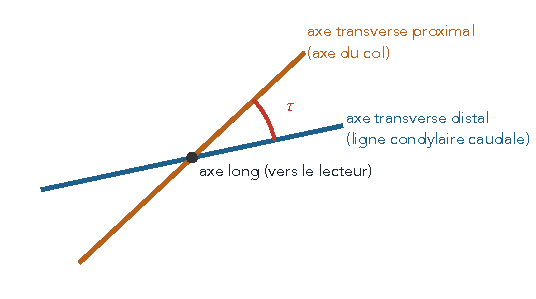
\includegraphics[width=0.5\linewidth]{torsion.pdf}
\caption{La torsion $\tau$ : l'angle, vu le long de l'axe de l'os, entre un axe transverse proximal et un axe transverse
distal.}
\label{fig:torsion}
\end{figure}

Le logiciel utilise les définitions publiées au scanner :
\begin{itemize}
  \item \textbf{fémur} (antéversion, Al Aiyan 2021 \cite{alaiyan2021}) : axe long = axe anatomique ; axe proximal = du
  centre de la tête à la base du col au niveau du petit trochanter ; axe distal = ligne des points caudaux des
  condyles ; $+$ = col dirigé vers crânial ;
  \item \textbf{tibia} (Brühschwein 2023 \cite{bruhschwein2023t}) : axe long par les centres de la diaphyse à 25 et
  75~\% de la longueur ; axe proximal = ligne des points caudaux des condyles ; axe distal = axe antécochléaire ;
  $-$ = interne, $+$ = externe.
\end{itemize}

\begin{exemple}
Lévrier : antéversion de 25,1\degre{} (normale : 20 à 35\degre) et torsion tibiale de $-7{,}9\degre$ (normale : $-10$
à $+2\degre$). Les anciennes définitions du prototype (axe du col au ras de la tête, axe bimalléolaire) donnaient
15,6\degre{} et $+6{,}0\degre$ : deux fausses « torsions externes » sur un chien sain. La définition compte autant que
la mesure.
\end{exemple}

\section{Valeurs normales et écart de définition}
\label{sec:calibration}

Les valeurs normales publiées sont mesurées sur radiographie, avec des repères placés à la main. Nos repères 3D n'ont
pas exactement la même définition. Comparer directement serait faux de plusieurs degrés pour certains angles de
profil, dont les lignes articulaires sont courtes (20 à 30~mm : 1~mm sur un bord arrondi change l'angle de 2 à
3\degre).

Nous mesurons donc l'\textbf{écart de définition} une fois pour toutes, sur l'os sain de l'os fictif, dont les repères
« radiographiques » sont connus :
\begin{gather}
  \Delta = \text{angle}(\text{repères détectés}) - \text{angle}(\text{repères du modèle}), \nonumber \\
  \text{valeur normale utilisée} = \text{valeur publiée} + \Delta.
\end{gather}
Comme les deux mesures sont faites sur le même os, l'écart ne vient que des définitions. Il est faible de face
(aLPFA $+0{,}15\degre$, aLDFA $+0{,}01\degre$, mMPTA $+1{,}30\degre$, mMDTA $+0{,}14\degre$) et plus grand de profil
(aCdDFA $-8{,}2\degre$, mCaPTA $+9{,}5\degre$, mCrDTA $+5{,}1\degre$). Le résultat est gardé en cache dans
\fichier{calibration_reperes.json} et recalculé si le code de l'étape 6 change.

\begin{table}[htbp]
\centering\small
\caption{Les angles du lévrier et les valeurs normales dans la définition du logiciel (moyenne ± écart-type). Un
angle est jugé anormal à plus de deux écarts-types.}
\label{tab:normales-levrier}
\begin{tabular}{llrrr}
\toprule
\titrecol{Os} & \titrecol{Angle} & \titrecol{Lévrier} & \titrecol{Normale} & \titrecol{Écart / écart-type} \\
\midrule
fémur & aLPFA & 114,2\degre & 103,2 ± 6,4\degre & $+1{,}7$ \\
 & aLDFA & 96,3\degre & 94,0 ± 3,3\degre & $+0{,}7$ \\
 & aCdDFA & 88,7\degre & 88,1 ± 6,3\degre & $+0{,}1$ \\
tibia & mMPTA & 91,2\degre & 94,6 ± 1,8\degre & $-1{,}9$ \\
 & mMDTA & 96,5\degre & 96,1 ± 2,7\degre & $+0{,}1$ \\
 & valgus tibial & 7,7\degre & 13,2 ± 3,1\degre & $-1{,}8$ \\
 & mCaPTA & 77,7\degre & 73,2 ± 2,6\degre & $+1{,}7$ \\
 & mCrDTA & 84,5\degre & 86,7 ± 3,2\degre & $-0{,}7$ \\
\bottomrule
\end{tabular}
\end{table}

\section{Choisir l'os à planifier}

Le chirurgien arrive en général avec \textbf{un scanner pour un os}. Le logiciel retient les fémurs et les tibias
complets. S'il y en a plusieurs, il propose le plus éloigné des normes (la somme des écarts en écarts-types). Si le
même os est complet des deux côtés, l'autre devient le \textbf{membre controlatéral}, la meilleure référence. Le choix
et sa raison sont écrits dans \fichier{cora_cas.json} et affichés dans la carte \ui{Os à planifier (CORA)}.

\section{Validation}

\begin{itemize}
  \item \textbf{Os fictif posé au hasard} (4 poses, dont 2 en miroir) : côté reconnu 8 fois sur 8 ; repères à moins de
  0,84~mm des repères exacts au fémur et de 0,98~mm au tibia ; mêmes repères dans les quatre poses (écart nul dans le
  repère de l'os).
  \item \textbf{Lévrier} : les trois os coupés par le champ sont refusés ; les angles du fémur et du tibia complets
  sont dans les normes ; l'os déplacé puis mis en miroir donne les mêmes repères.
\end{itemize}

\begin{danslecode}
\fichier{code_source/etape6_reperes.py} : classe \code{Os} (repère courant, \code{poser()}, \code{section_remplie()},
\code{milieu_diaphyse()}), \code{orienter()}, \code{extremites_coupees()}, \code{analyser()} (les trois passes),
\code{reperes_femur()}, \code{reperes_tibia()}, \code{enveloppe_tangente()}, \code{sphere_robuste()},
\code{region_connexe()}, \code{angles_articulaires()}, \code{torsion()}, \code{calibration()}, \code{normales()},
\code{choisir_cible()}. Sorties : \fichier{cora_<os>.json}, \fichier{cora_<os>.bin} (maillage dans le repère de l'os),
\fichier{cora_<os>.png}, \fichier{cora_cas.json}.
\end{danslecode}

\chapter{La planification CORA en 3D}
\label{chap:planification}

\begin{chapeau}
C'est le cœur du projet. À partir de l'os et de ses repères, la planification construit les axes des deux segments,
trouve le CORA et l'angle vrai, place la charnière et les traits de coupe, calcule la correction (avec la dérotation),
place les broches, choisit la voie d'abord et le type de coin, puis écrit la prescription. Tout est calculé dans le
fichier JavaScript \fichier{code_source/cora/app/cora_simple.js} (fonction \code{planifier()}), qui ne fait aucun
dessin : il peut être testé seul, sous Node.
\end{chapeau}

\section{Les axes des deux segments}
\label{sec:axes}

L'os déformé est vu comme deux segments droits. Il faut l'axe de chacun. Paley le construit à partir de la ligne
articulaire de l'extrémité et de l'angle articulaire \emph{normal} \cite{paley2002}. Le logiciel offre deux
références.

\subsection{Référence « os sain »}

Si l'on dispose d'un os sain du même animal (le membre controlatéral), ou de l'os avant une déformité de test, on
mémorise la position de son axe par rapport à ses articulations, puis on la reporte sur l'os déformé. Pour une
articulation, on construit un repère local avec ses deux lignes articulaires :
\begin{equation}
  \vb{e}_1 = \frac{\vb{J}_F}{\norm{\vb{J}_F}}, \qquad
  \vb{e}_3 = \frac{\vb{J}_S - (\vb{J}_S\cdot\vb{e}_1)\,\vb{e}_1}{\norm{\ldots}}, \qquad
  \vb{e}_2 = \vb{e}_3 \times \vb{e}_1,
\end{equation}
où $\vb{J}_F$ est la ligne articulaire de face (de médial à latéral) et $\vb{J}_S$ celle de profil (de crânial à
caudal). L'axe sain s'écrit dans ce repère local ; sur l'os déformé, on reconstruit le même repère local avec ses
propres lignes articulaires et on y replace l'axe. C'est l'équivalent 3D de « ligne articulaire + angle normal ».

\subsection{Référence « valeurs normales » (méthode de Paley)}

Sans os sain, on construit l'axe dans chaque vue. Dans la vue de face, on tourne la direction de la ligne articulaire
de l'angle normal, dans un sens puis dans l'autre, et on garde la direction qui va vers distal et qui est la plus
proche de la verticale. On fait de même de profil. On obtient deux directions 2D, $\vb{d}_F = (d_{F,x}, d_{F,y})$ de
face et $\vb{d}_S = (d_{S,z}, d_{S,y})$ de profil, qu'on combine en une direction 3D dont elles sont les projections :
\begin{equation}
  \vb{d} = \frac{\bigl(d_{F,x}/\abs{d_{F,y}},\ -1,\ d_{S,z}/\abs{d_{S,y}}\bigr)}{\norm{\ldots}}.
  \label{eq:dir3d}
\end{equation}
Au tibia, les axes passent par l'éminence (segment proximal) et par le centre distal (segment distal). Au fémur, l'axe
proximal est l'axe anatomique mesuré ; l'axe distal a la direction donnée par les lignes articulaires distales, et sa
position est fixée de face par l'os fictif (il coupe la ligne des condyles au même endroit que l'axe sain), et de
profil par la règle « une seule angulation » : le CORA de profil est au même niveau que le CORA de face.

\begin{pourquoi}
\textbf{Pourquoi cette règle de profil au fémur ?} Le fémur du chien est arqué vers l'avant : chez le lévrier, les
condyles sont 33~mm en arrière de l'axe proximal. Un gabarit de profil tiré d'un autre os serait donc faux d'un chien à
l'autre. Pour une déformité à un seul apex, les CORA de face et de profil sont au même niveau : c'est une hypothèse
plus sûre.
\end{pourquoi}

\section{Le CORA en 3D}
\label{sec:cora3d}

\subsection{Deux droites qui ne se coupent pas}

En 3D, deux axes mesurés ne se coupent presque jamais exactement : ils passent l'un à côté de l'autre. On cherche le
point où ils sont le plus proches. Soient l'axe proximal $\vb{p} + s\,\vb{u}$ et l'axe distal $\vb{q} + t\,\vb{v}$
(\cref{fig:perp-commune}). On minimise
\begin{equation}
  f(s, t) = \norm{\vb{w}_0 + s\,\vb{u} - t\,\vb{v}}^2, \qquad \vb{w}_0 = \vb{p} - \vb{q}.
\end{equation}
En annulant les dérivées par rapport à $s$ et à $t$, on obtient un système $2 \times 2$. Avec $a = \vb{u}\cdot\vb{u}$,
$b = \vb{u}\cdot\vb{v}$, $c = \vb{v}\cdot\vb{v}$, $d = \vb{u}\cdot\vb{w}_0$ et $e = \vb{v}\cdot\vb{w}_0$ :
\begin{equation}
  \tcbhighmath{s^* = \frac{b\,e - c\,d}{a\,c - b^2}, \qquad t^* = \frac{a\,e - b\,d}{a\,c - b^2}.}
  \label{eq:perp}
\end{equation}
Les points $P_p = \vb{p} + s^*\vb{u}$ et $P_d = \vb{q} + t^*\vb{v}$ sont les pieds de la \emph{perpendiculaire
commune}. Le CORA est leur milieu, $C = (P_p + P_d)/2$, et $\delta = \norm{P_p - P_d}$ dit de combien les axes se
ratent. Si $a\,c - b^2 \approx 0$, les axes sont parallèles : il n'y a pas d'angulation.

\fig{perpendiculaire_commune.pdf}{Le CORA en 3D : le milieu de la perpendiculaire commune aux deux
axes.}{fig:perp-commune}

\subsection{Quand il n'y a pas de CORA}

Si l'angle entre les axes est inférieur à 0,5\degre, ou si le CORA tombe hors de l'os (au-delà de 4 à 96~\% de sa
longueur), il n'y a pas d'ostéotomie au CORA possible. C'est le cas des os sains du lévrier : le logiciel l'indique
(« pas de correction indiquée ») au lieu de proposer une coupe absurde.

\section{L'angle vrai et le plan de la déformité}
\label{sec:angle-vrai}

L'angle vrai est simplement l'angle entre les deux directions :
\begin{equation}
  \theta = \arccos(\vb{u}\cdot\vb{v}).
\end{equation}
Les composantes $F$ et $S$ sont les angles orientés entre les projections de $\vb{u}$ et $\vb{v}$ dans chaque vue. De
face, $F < 0$ indique un varus (le bas part vers médial) ; de profil, $S > 0$ un procurvatum.

\textbf{Démonstration de $\tan^2\theta = \tan^2 F + \tan^2 S$.} Prenons l'axe proximal vertical,
$\vb{u} = (0, -1, 0)$. Une direction distale dont les angles projetés valent $F$ de face et $S$ de profil a pour
vecteur directeur $\vb{v} \propto (\pm\tan F,\ -1,\ \pm\tan S)$ : de face, on ne voit que $(\pm\tan F, -1)$, qui fait
bien l'angle $F$ avec la verticale ; de profil, $(\pm\tan S, -1)$. Alors
\begin{equation}
  \tcbhighmath{\cos\theta = \frac{\vb{u}\cdot\vb{v}}{\norm{\vb{v}}} = \frac{1}{\sqrt{1 + \tan^2 F + \tan^2 S}}
  \quad\Longrightarrow\quad
  \tan^2\theta = \frac{1}{\cos^2\theta} - 1 = \tan^2 F + \tan^2 S.}
\end{equation}
Le logiciel n'a pas besoin de cette formule, puisqu'il calcule $\theta$ directement en 3D ; elle sert de contrôle et
d'explication (\cref{fig:angle-vrai}). L'orientation du plan de la déformité par rapport au plan frontal est
$\varphi = \arctan\bigl(\abs{\tan S}/\abs{\tan F}\bigr)$.

\fig{angle_vrai.pdf}{À gauche, les projections $F$ et $S$ et l'angle vrai $\theta$. À droite, l'angle vrai en
fonction de $F$ pour plusieurs valeurs de $S$ : il est toujours inférieur à la somme $F + S$ (en tirets).}{fig:angle-vrai}

\section{La bissectrice, l'ACA et la rotation}
\label{sec:bissectrice}

Les deux axes définissent le plan de la déformité. Trois directions servent ensuite (\cref{fig:bissectrice}a) :
\begin{equation}
  \vb{n}_{\text{ACA}} = \frac{\vb{u}\times\vb{v}}{\norm{\vb{u}\times\vb{v}}}, \qquad
  \vb{b} = \frac{\vb{u} + \vb{v}}{\norm{\vb{u} + \vb{v}}}, \qquad
  \vb{c} = \frac{\vb{u} - \vb{v}}{\norm{\vb{u} - \vb{v}}}.
\end{equation}
$\vb{n}_{\text{ACA}}$ est perpendiculaire au plan de la déformité : c'est la direction de l'axe de correction.
$\vb{b}$ est la normale du \emph{plan bissecteur}, qui partage l'angle entre les segments. $\vb{c}$ est la
\emph{bissectrice transverse}, dans le plan de la déformité, dirigée vers le côté convexe. Le logiciel coupe l'os par
le plan bissecteur passant par le CORA : il en tire la largeur de l'os le long de $\vb{c}$ (distances aux corticales
convexe et concave) et sa profondeur le long de l'ACA.

\subsection{La formule de Rodrigues}

La correction fait tourner le segment distal d'un angle $\theta$ autour de l'axe unitaire
$\vb{k} = (\vb{v}\times\vb{u})/\norm{\vb{v}\times\vb{u}}$, qui amène $\vb{v}$ sur $\vb{u}$. La matrice de rotation
d'angle $\alpha$ autour de $\vb{k}$ est donnée par la formule de Rodrigues \cite{rodrigues1840} :
\begin{equation}
  \tcbhighmath{\mt{R}(\vb{k}, \alpha) = \mt{I} + \sin\alpha\,[\vb{k}]_\times + (1 - \cos\alpha)\,[\vb{k}]_\times^2,
  \qquad
  [\vb{k}]_\times = \begin{pmatrix} 0 & -k_z & k_y \\ k_z & 0 & -k_x \\ -k_y & k_x & 0 \end{pmatrix}.}
  \label{eq:rodrigues}
\end{equation}
Une rotation autour d'une droite qui passe par le point $Q$ envoie $\vb{x}$ sur
$\mt{R}(\vb{x} - Q) + Q$ : c'est une transformation rigide $\mt{T} = (\mt{R}, \vb{t})$ avec $\vb{t} = Q - \mt{R}Q$.
Deux transformations se composent par $\mt{T}_A \circ \mt{T}_B = (\mt{R}_A\mt{R}_B,\ \mt{R}_A\vb{t}_B + \vb{t}_A)$, et
l'inverse est $(\mt{R}^{\mathsf T}, -\mt{R}^{\mathsf T}\vb{t})$.

\section{L'ostéotomie : charnière, traits et coin}
\label{sec:traits}

\subsection{La charnière}

La charnière $H$ est placée sur la bissectrice transverse, au niveau du CORA, à une profondeur $h$ (2~mm par défaut)
à l'intérieur de la corticale opposée au coin :
\begin{equation}
  H = P_c + \sigma\,(\ell - h)\,\vb{c},
  \qquad
  \begin{cases}
    \sigma = -1,\ \ell = \text{distance à la corticale concave} & \text{coin de fermeture,} \\
    \sigma = +1,\ \ell = \text{distance à la corticale convexe} & \text{coin d'ouverture,}
  \end{cases}
\end{equation}
où $P_c$ est le centre de la section. La lame entre de l'autre côté : par la corticale convexe pour une fermeture, par
la corticale concave pour une ouverture. On note $D = \text{largeur} - h$ la distance de la charnière à la corticale
d'entrée.

\begin{pourquoi}
\textbf{Pourquoi 2~mm ?} À cet endroit, la charnière est l'ACA de Paley : aucune translation. Et il reste un pont d'os
cortical assez fin pour plier sans casser (au plus 3~mm), qui garde les fragments en contact. Au-delà de 3~mm, le pont
ne plie plus : l'ostéotomie devient complète et le coin devient \emph{mixte} (une partie se ferme, l'autre s'ouvre).
\end{pourquoi}

\subsection{Les traits de coupe}

\begin{itemize}
  \item \textbf{Coin de fermeture} : deux plans passant par $H$, de normales $\vb{u}$ et $\vb{v}$ (l'un est
  perpendiculaire à l'axe proximal, l'autre à l'axe distal). Le coin d'os entre les deux est retiré.
  \item \textbf{Coin d'ouverture} : un seul plan passant par $H$, de normale $\vb{b}$ (le plan bissecteur).
\end{itemize}

\fig{bissectrice_coins.pdf}{(a) Le plan de la déformité : axes, CORA, bissectrice transverse. (b) Le coin de fermeture
et sa base. (c) Le coin d'ouverture et l'écart qu'il crée.}{fig:bissectrice}

\subsection{La taille du coin}

\textbf{Fermeture.} Prenons un point à la distance $D$ de $H$ le long de $\vb{c}$, et mesurons l'écart entre les deux
plans le long de $\vb{b}$. Un point $H + D\,\vb{c} + w\,\vb{b}$ est sur le plan de normale $\vb{u}$ si
$D\,(\vb{c}\cdot\vb{u}) + w\,(\vb{b}\cdot\vb{u}) = 0$. Or $\vb{c}\cdot\vb{u} = \sin(\theta/2)$ et
$\vb{b}\cdot\vb{u} = \cos(\theta/2)$, d'où $w = -D\tan(\theta/2)$ ; de même $w = +D\tan(\theta/2)$ pour le plan de
normale $\vb{v}$. La base du coin, à la corticale d'entrée, vaut donc
\begin{equation}
  \tcbhighmath{\text{base}_{\text{fermeture}} = 2\,D\,\tan(\theta/2).}
\end{equation}

\textbf{Ouverture.} Un point de la face coupée, à la distance $D$ de la charnière, décrit un arc de cercle d'angle
$\theta$ : la corde de cet arc est l'ouverture
\begin{equation}
  \tcbhighmath{\text{ouverture} = 2\,D\,\sin(\theta/2).}
\end{equation}

\begin{exemple}
Tibia de 16~mm de large, charnière à 2~mm, $\theta = 20\degre$ : $D \approx 14$~mm, base du coin de fermeture
$2 \times 14 \times \tan 10\degre \approx 4{,}9$~mm, ouverture $2 \times 14 \times \sin 10\degre \approx 4{,}9$~mm. Pour un
petit angle, les deux sont proches. Il faut au moins 1,5~mm de matière entre les deux fentes du guide : un coin de
fermeture trop fin est déconseillé (\cref{sec:choix-coin}).
\end{exemple}

\subsection{Rester loin du cartilage}

Un trait de coupe doit rester à au moins 5~mm du cartilage articulaire, et un coin de fermeture ne doit pas en
emporter. Si le CORA est trop près de l'articulation (par exemple dans la trochlée du fémur), le logiciel déplace la
coupe vers la diaphyse, millimètre par millimètre, jusqu'à 35~\% de la longueur de l'os : c'est la règle 2.

\section{La règle 2 : couper ailleurs qu'au CORA}
\label{sec:regle2}

Quand la coupe est déplacée de $z$~mm le long de l'os, la charnière $H$ n'est plus sur la bissectrice du CORA. Paley
impose alors que l'\textbf{ACA reste sur la bissectrice} : sinon les axes ne seraient pas réalignés (règle 3).

\textbf{Pourquoi tout point de la bissectrice convient.} Soit $Q = C + \lambda\,\vb{c}$ un point de la bissectrice et
$\mt{R}$ la rotation d'angle $\theta$ qui amène $\vb{v}$ sur $\vb{u}$. Elle envoie la direction distale sur
$\vb{u}$ ; il reste à vérifier que l'axe distal tombe sur l'axe proximal. Le point $C$, commun aux deux axes, va en
$C' = C + \lambda\,(\vb{c} - \mt{R}\vb{c})$. Dans le plan de la déformité, $\vb{v}$ est $\vb{u}$ tourné de $-\theta$
et $\mt{R}\vb{u}$ est $\vb{u}$ tourné de $+\theta$, donc $\vb{v} + \mt{R}\vb{u} = 2\cos\theta\,\vb{u}$. Comme
$\vb{c} \propto \vb{u} - \vb{v}$ et $\mt{R}\vb{c} \propto \mt{R}\vb{u} - \vb{u}$ :
\begin{equation}
  \vb{c} - \mt{R}\vb{c} \propto 2\vb{u} - (\vb{v} + \mt{R}\vb{u}) = 2(1 - \cos\theta)\,\vb{u}.
\end{equation}
$C'$ est donc sur l'axe proximal, et l'axe distal corrigé est confondu avec lui, quel que soit $\lambda$.

\textbf{Le bon point.} Parmi ces points, le logiciel prend celui qui garde les faces de l'ostéotomie en contact : la
charnière doit rester sur le plan de la face proximale (de normale $\vb{n}_F$ : $\vb{u}$ en fermeture, $\vb{b}$ en
ouverture). La condition $(\mt{R}(H - Q) + Q - H)\cdot\vb{n}_F = 0$ donne
\begin{equation}
  \lambda = \frac{\bigl((\mt{R} - \mt{I})(H - C)\bigr)\cdot\vb{n}_F}{\bigl((\mt{R} - \mt{I})\,\vb{c}\bigr)\cdot\vb{n}_F}.
\end{equation}
Le fragment distal glisse alors le long de la coupe : c'est la \textbf{translation à l'ostéotomie}, mesurée par
$\norm{\mt{T}(H) - H}$ (\cref{fig:regle2}). Au-delà de 50~\% de la largeur de l'os, le contact osseux devient
insuffisant : le logiciel le signale comme bloquant.

\fig{regle2.pdf}{Règle 1 et règle 2 (coin d'ouverture). En coupant 22~mm sous le CORA, les axes sont toujours
réalignés, mais le fragment distal (en bleu) glisse le long de la coupe.}{fig:regle2}

\section{La dérotation}
\label{sec:derotation}

Si la torsion doit être corrigée, le fragment distal tourne en plus autour de son axe, d'un angle $\alpha$. La
\textbf{cible} dépend de la référence : la torsion de l'os sain, ou, avec les valeurs normales, la valeur moyenne
publiée seulement si la torsion sort des seuils. La décision se prend sur la torsion \emph{après} la seule correction
angulaire : une angulation pure incline un peu les axes transverses et crée quelques dixièmes de degré de « fausse
torsion », que la correction annule.

La dérotation tourne autour d'un axe que la correction garde aligné :
\begin{itemize}
  \item \textbf{fermeture} : autour de l'axe distal, \emph{avant} la fermeture, $\mt{T} = \mt{T}_{\text{angle}} \circ
  \mt{R}_\alpha$ ; la face distale, perpendiculaire à cet axe, tourne dans son plan ;
  \item \textbf{ouverture} : autour de l'axe réaligné (l'axe proximal), \emph{après} l'ouverture,
  $\mt{T} = \mt{R}_\alpha \circ \mt{T}_{\text{angle}}$.
\end{itemize}

L'angle $\alpha$ est cherché par la \textbf{méthode de la sécante} \cite{press2007}, pour que la torsion mesurée après
la correction, $\tau(\alpha)$, égale la cible $\tau^*$. Avec $f(\alpha) = \tau(\alpha) - \tau^*$ :
\begin{equation}
  \alpha_{n+1} = \alpha_n - f(\alpha_n)\,\frac{\alpha_n - \alpha_{n-1}}{f(\alpha_n) - f(\alpha_{n-1})}.
\end{equation}
Comme $\tau$ dépend presque linéairement de $\alpha$, deux ou trois itérations suffisent (au plus six, arrêt à
0,001\degre). On ne dérote pas en dessous de 1\degre. Une dérotation impose une ostéotomie complète : une charnière
corticale ne peut pas tourner sur elle-même.

\section{Les broches}
\label{sec:broches}

Les broches relient la planification au geste : elles fixent le guide, puis servent de repère pour la correction et
de support pour la réduction. Leur direction et leur position sont calculées ici.

\subsection{L'astuce de l'inverse}

Les broches ont quatre rôles : fixer le guide de coupe, porter la correction, tenir la réduction et bloquer la
rotation. L'astuce est de forer les broches distales avec l'\textbf{inverse de la correction}. Si $\vb{d}$ est la
direction des broches proximales et $\mt{R}_T$ la rotation de la correction complète (angle et dérotation), les
broches distales sont forées selon
\begin{equation}
  \vb{d}_{\text{dist}} = \mt{R}_T^{-1}\,\vb{d}
  \quad\Longrightarrow\quad
  \text{après correction : } \mt{R}_T\,\vb{d}_{\text{dist}} = \vb{d}.
\end{equation}
Après la correction, \textbf{toutes les broches sont parallèles}, et seulement si la correction est la bonne. Le
chirurgien a un repère visuel immédiat, et le guide de réduction (\cref{sec:reduction}) peut s'y enfiler.

\fig{broches.pdf}{Les broches distales, forées avec l'inverse de la correction, deviennent parallèles aux broches
proximales quand la correction est exacte.}{fig:broches}

\subsection{Où placer les broches}

Le logiciel cherche une position pour chaque broche dans un grand nombre de possibilités, et garde la première qui
respecte toutes les règles :
\begin{itemize}
  \item \textbf{position le long de l'os} : à une distance de la coupe de 1,2 fois la largeur locale de l'os si la
  place le permet, sinon plus près, jamais contre la tour de fente ;
  \item \textbf{une broche par fragment} (une proximale, une distale), sur la ligne centrale de l'os, ou décalée de 2 à
  4~mm si un obstacle l'impose ;
  \item \textbf{direction} : vers l'os depuis la face d'appui du guide, tournée autour de l'os d'un angle $\beta$ de
  0 à $\pm 45\degre$ (par pas de 5\degre), puis inclinée le long de l'os de $\gamma = \pm 10$ ou $\pm 20\degre$ si le
  retrait du guide l'exige ;
  \item \textbf{hauteur des manchons} : 15~mm, raccourcis à 10 puis 8~mm si un manchon heurte la tour de fente.
\end{itemize}

\begin{table}[htbp]
\centering\small
\caption{Les règles qu'une broche doit respecter.}
\label{tab:regles-broches}
\begin{tabularx}{\linewidth}{L{4.4cm}Y}
\toprule
\titrecol{Règle} & \titrecol{Valeur} \\
\midrule
traverser l'os (bicorticale) & au moins 5~mm d'os le long de la broche \\
rester loin des plans de coupe & 2~mm de pont osseux, du bon côté ; pointe hors du trajet de la lame de l'autre trait \\
rester loin du cartilage & 3~mm de l'axe de la broche ; manchon jamais posé sur le cartilage \\
éviter les os voisins & 2~mm de l'axe, jusqu'à 8~mm au-delà de la corticale opposée (un forage un peu trop long n'embroche pas la fibula) \\
entrer franchement dans la corticale & moins de 50\degre{} entre la broche et la normale à l'os (sinon la mèche glisse) \\
laisser sortir le guide & une des deux moitiés doit s'éloigner de l'autre en sortant (dérive inférieure à 0,03, environ 2\degre) \\
\bottomrule
\end{tabularx}
\end{table}

Deux autres configurations existent : \textbf{1 + 1} (une broche par fragment ; chaque fragment peut alors tourner
autour de sa broche) et \textbf{1 + 2} (une proximale, deux distales côte à côte, utile pour un fragment distal court).

\begin{danslecode}
\code{placerBroches()}, \code{evaluerBroche()} et \code{manchonLibre()}. La recherche évalue des milliers de
positions ; chaque contrôle parcourait tous les sommets de l'os, du cartilage et des voisins (environ 40~s sur un fémur).
Les points sont maintenant rangés une fois dans une grille de cellules de 1,5~mm, et une requête n'examine que les
cellules utiles, avec le même test point par point : mêmes résultats, beaucoup plus vite (\code{grille()},
\code{parcourirLeLong()}).
\end{danslecode}

\section{Où poser le guide : la voie d'abord}
\label{sec:abord}

La lame entre toujours du côté \textbf{opposé à la charnière}, par la \emph{face du coin} : convexe en fermeture,
concave en ouverture. Le guide se pose sur cette face. Mais elle doit être accessible par une voie d'abord habituelle
(\cref{tab:abords}).

\begin{table}[htbp]
\centering\small
\caption{Les secteurs où le guide peut être posé (choix raisonnés du projet, à valider avec un chirurgien).}
\label{tab:abords}
\begin{tabularx}{\linewidth}{lL{3.2cm}Y}
\toprule
\titrecol{Os} & \titrecol{Abord (demi-ouverture)} & \titrecol{Structures à protéger} \\
\midrule
fémur & latéral (± 60\degre) & nerf sciatique en arrière du fémur ; vaste latéral et biceps fémoral \\
 & médial (± 45\degre) & artère et veine fémorales, nerf saphène ; artère génienne descendante \\
tibia & médial (± 60\degre) & veine et artère saphènes, nerf saphène ; derrière l'os, artères poplitée et tibiale crâniale \\
 & latéral (± 30\degre) & muscles tibial crânial et extenseurs ; artère tibiale crâniale et nerf fibulaire \\
\bottomrule
\end{tabularx}
\end{table}

Le logiciel cherche, dans chaque secteur, la direction la plus proche de la face du coin, par pas de 5\degre, telle
qu'aucun os voisin ne soit sur le trajet de la lame. Trois cas :
\begin{itemize}
  \item la face du coin est accessible : le guide s'y pose et la charnière peut être conservée ;
  \item une face accessible est à moins de 60\degre{} de la face du coin : le guide s'y pose, mais l'ostéotomie
  devient complète ;
  \item sinon, la lame entrerait du côté de la charnière : ce coin est déclaré \textbf{non réalisable par un abord
  usuel}, et l'autre type de coin est recommandé. Si en plus un os voisin (en général la fibula) est sur le trajet de
  la lame, \textbf{aucun guide n'est construit} : il occuperait l'espace entre les deux os, où l'on ne peut ni le
  glisser, ni le fixer, ni couper.
\end{itemize}

\section{La stratégie chirurgicale}
\label{sec:strategie}

\subsection{Les contraintes au niveau de la coupe}

Pour chaque coin, le logiciel liste ce qui pourrait empêcher de couper à ce niveau, par gravité (bloquant, attention,
information) :
\begin{itemize}
  \item cartilage et capsule articulaire : au moins 5~mm du trait ;
  \item tubérosité tibiale (insertion du ligament de la rotule) : au moins 8~mm ;
  \item épicondyles du fémur (origine des ligaments collatéraux) : au moins 6~mm ;
  \item physes d'un chien en croissance (zones approchées en fraction de la longueur) ;
  \item place pour la fixation : au moins 25~mm d'os de chaque côté (plaque à trois vis et broches) ;
  \item consolidation : rapide en métaphyse, plus lente en diaphyse et au tiers distal du tibia ;
  \item translation de la règle 2 (attention au-delà de 25~\% de la largeur, bloquant au-delà de 50~\%) ;
  \item structures à protéger pendant l'abord (\cref{tab:abords}).
\end{itemize}

\subsection{Ouverture ou fermeture ?}
\label{sec:choix-coin}

Le logiciel compare les deux coins critère par critère, dans un ordre fixé. Le premier critère qui les départage
décide ; tous restent affichés à l'écran (\cref{fig:choix-coin}) :
\begin{enumerate}
  \item \textbf{accès} : la lame entre par un abord usuel, du côté opposé à la charnière ;
  \item \textbf{charnière conservée} (stabilité, pas de translation) ;
  \item \textbf{règle 1} plutôt que règle 2 ;
  \item un coin de fermeture \textbf{assez épais} pour deux fentes (au moins 1,5~mm de matière entre elles) ;
  \item une \textbf{ouverture raisonnable} (au plus 40~\% de la largeur de l'os ; au-delà, greffe et consolidation
  longue) ;
  \item la \textbf{longueur} : si le membre opéré est plus court (ou plus long) que l'autre d'au moins 3~mm, le coin qui
  compense le mieux (la fermeture raccourcit, l'ouverture allonge) ;
  \item à défaut, la \textbf{fermeture} : surfaces d'os en contact, stabilité immédiate, pas de greffe.
\end{enumerate}

\fig[0.92]{choix_du_coin.pdf}{Comment le logiciel choisit entre le coin de fermeture et le coin
d'ouverture.}{fig:choix-coin}

\begin{exemple}
Sur 606 cas simulés (\cref{sec:campagne-strategie}), les choix suivent la pratique publiée : au tibia, un valgus se
corrige par fermeture et un varus par ouverture (le critère décisif est l'accès : la face médiale du tibia) ; au fémur,
la fermeture domine (critère de stabilité) \cite{petazzoni2012,brower2017}.
\end{exemple}

\section{La prescription}

La planification se termine par un fichier \fichier{prescription.json} (format v2.2), qui contient tout ce que l'étape
7 doit savoir : la déformité, la stratégie, la charnière, les plans de coupe et leur profondeur, la correction (matrice
$4 \times 4$ et dérotation), les broches et leur position après correction, la face d'appui, les contraintes et les
alertes. Il est décrit en détail à l'\cref{ann:prescription}. Pour un os segmenté, il contient aussi la matrice qui
ramène le repère de l'os à celui du scanner : le guide peut ainsi être superposé au STL de l'os dans 3D Slicer.

\section{Les déformités simulées}
\label{sec:deformite-simulee}

Pour tester la méthode, on impose à un os sain une déformité connue (fonction \code{makeDeformity()}). L'apex $A$ est
placé à une fraction choisie de la longueur. La direction distale est
\begin{equation}
  \vb{v}_0 = \frac{(-s_F\tan F,\ -1,\ s_S\tan S)}{\norm{\ldots}},
\end{equation}
avec $s_F = +1$ en varus, $-1$ en valgus, et $s_S = +1$ en procurvatum, $-1$ en recurvatum : ainsi, les angles projetés
valent \emph{exactement} $F$ et $S$. Le segment distal tourne de $\theta = \arccos(\vb{u}_0\cdot\vb{v}_0)$ autour de
$\vb{n} = \vb{u}_0\times\vb{v}_0$ passant par l'apex, après une éventuelle torsion $\tau$ autour de l'axe sain. Pour
éviter une cassure, la rotation est appliquée progressivement dans une zone de transition de largeur $w$ autour de
l'apex, avec le poids
\begin{equation}
  \omega(t) = t^2\,(3 - 2t), \qquad t = \clamp\!\left(\frac{y_A + w/2 - y}{w},\ 0,\ 1\right),
\end{equation}
où $y$ est la hauteur du point. Les 17 \textbf{préréglages cliniques} de l'application (valgus proximal du tibia, pes
varus du teckel, varus du fémur distal de la luxation de la rotule\ldots) sont des déformités de ce type, avec leur
contexte et leur traitement publié.

\section{Les 13 étapes à l'écran}

Dans l'application, la planification est découpée en 13 étapes. Chacune montre l'os en 3D, avec un texte qui
explique ce qui se passe et ses sources (\cref{tab:13etapes}, \cref{fig:capture-angle-vrai}).

\begin{table}[htbp]
\centering\small
\caption{Les 13 étapes de l'onglet \ui{Planification CORA}.}
\label{tab:13etapes}
\begin{tabularx}{\linewidth}{rL{4cm}Y}
\toprule
& \titrecol{Étape} & \titrecol{Ce qu'elle montre} \\
\midrule
1 & Le cas & l'os, ses repères, son côté, le dépistage des angles (± 2 écarts-types) \\
2 & Face : lignes articulaires & les lignes d'orientation articulaire de face \\
3 & Face : angles articulaires & l'axe et les angles de face, comparés aux normes \\
4 & Face : axes et CORA & les axes des segments et le CORA de face \\
5 & Profil : lignes et angles & les lignes articulaires et les angles de profil \\
6 & Profil : axes et CORA & les axes et le CORA de profil \\
7 & Angle vrai (3D) & l'angle vrai et le plan oblique de la déformité \\
8 & Bissectrice et ACA & le plan bissecteur et l'axe de correction \\
9 & Angle et traits de coupe & la charnière, les plans de coupe, le coin \\
10 & Correction & la correction animée, avec la dérotation et les broches \\
11 & Contrôle & les angles après correction, dans les deux plans \\
12 & Guides de coupe & la prescription, la construction des guides, les contrôles, les fichiers \\
13 & Et la torsion ? & la torsion mesurée, et pourquoi la radiographie ne suffit pas \\
\bottomrule
\end{tabularx}
\end{table}

\fig{capture_angle_vrai.png}{L'étape 7 de l'application : un tibia avec 15\degre{} de varus et 10\degre{} de
procurvatum. La déformité est dans un plan oblique (en rose) et l'angle vrai vaut 17,8\degre.}{fig:capture-angle-vrai}

\begin{danslecode}
\fichier{code_source/cora/app/cora_simple.js} : \code{reference()} et \code{axesNormales()} (les deux références),
\code{coraPerpCommune()} (\cref{eq:perp}), \code{planifier()} (tout le calcul), \code{M3.axisAngle()} (Rodrigues),
\code{RT.aboutAxis()} et \code{RT.compose()}, \code{choisirAbord()}, \code{contraintesCoupe()},
\code{recommanderCoin()}, \code{placerBroches()}, \code{mesuresTorsion()}, \code{makeDeformity()},
\code{prescription()}. L'interface des 13 étapes est dans \fichier{code_source/cora/app/modules/40_etapes.js}.
\end{danslecode}

\chapter{Étape 7 — Construire les guides imprimables}
\label{chap:guides}

\begin{chapeau}
Cette étape transforme la prescription en deux pièces à imprimer : un \textbf{guide de coupe}, qui guide la scie et
les broches, et un \textbf{guide de réduction}, qui tient les fragments dans la position corrigée pendant la fixation.
Chaque pièce est ensuite vérifiée par des contrôles indépendants de sa construction.
\end{chapeau}

\begin{figure}[htbp]
\centering
\tikz\node[fill=grisfond, rounded corners=6pt, inner xsep=10pt, inner ysep=10pt]{%
  \panneau{8.3cm}{rendu_face.png}{a}{face d'appui}\hspace{12pt}%
  \panneau{8.3cm}{rendu_profil.png}{b}{profil}\hspace{12pt}%
  \panneau{8.3cm}{rendu_reduction.png}{c}{guide de réduction}\hspace{12pt}%
  \panneau{8.3cm}{rendu_fermeture.png}{d}{coin de fermeture}};
\caption{Les guides construits par le logiciel sur un tibia (os fictif). (a) à (c) : coin d'ouverture posé par la
face médiale. (a) Le guide de coupe vu de sa face d'appui (bleu : moitié proximale ; vert : moitié distale ; orange :
ponts sécables). (b) Le profil, avec les broches. (c) Après la coupe et la correction : les broches sont parallèles et
le guide de réduction (violet) s'y enfile jusqu'à l'os corrigé. (d) Le guide de coupe d'un coin de fermeture : deux
moitiés, la partie au-dessus du coin osseux appartient à la moitié distale ; la fibula, qui passerait devant le guide
dans cette vue, n'est pas dessinée.}
\label{fig:guide-v3}
\end{figure}

\section{Ce que l'on construit}

Le \textbf{guide de coupe} est une \textbf{coque} moulée sur l'os, qui ne s'emboîte que dans une seule position.
Elle porte :
\begin{itemize}
  \item une \textbf{tour} par trait de coupe, percée d'une \textbf{fente} de 0,8~mm (lame de 0,6~mm et 0,2~mm de jeu)
  exactement dans le plan prescrit : une fente pour un coin d'ouverture, deux pour un coin de fermeture ;
  \item des \textbf{manchons}, un par broche (une par fragment), percés à 1,8~mm pour des broches de
  1,6~mm ;
  \item deux \textbf{ponts sécables}, petits morceaux de 2 × 5~mm aux deux bouts de la première fente, qui relient les
  deux moitiés et que l'on coupe à la pince après la coupe de l'os.
\end{itemize}

Les broches distales ne sont pas parallèles aux broches proximales avant la correction (\cref{sec:broches}). Le guide
de coupe est donc fait de deux moitiés : chacune sort en glissant le long de \emph{sa} broche. Après la correction, les deux broches sont parallèles : le \textbf{guide de réduction}, une barre à
deux manchons parallèles, s'enfile alors sur elles (\cref{sec:reduction}).

\begin{pourquoi}
\textbf{Pourquoi deux pièces simples ?} La version précédente du guide (octobre 2026) réglait aussi la profondeur de
coupe par la hauteur des tours (une graduation de lame gravée sur les tours) et transformait ses deux moitiés en verrou
de réduction (des oreilles percées d'un trou commun dans la seule position corrigée). Ces fonctions ajoutaient des
pièces, des réglages et des étapes au bloc opératoire, pour un gain qui restait à prouver sur un vrai os. Le
06/11/2026, nous avons choisi de revenir à un guide de coupe et un guide de réduction simples, le système le plus
utilisé dans les publications (\cref{chap:etat}) : moins de pièces à imprimer, un mode opératoire de 9 ou 10 étapes au
lieu de 12 à 15, et un code plus court (2\,032 lignes au lieu de 2\,827).
\end{pourquoi}

\section{Le principe : la modélisation implicite}
\label{sec:implicite}

Un solide peut être décrit par une fonction $F$ définie dans tout l'espace : $F(\vb{x}) < 0$ à l'intérieur,
$F(\vb{x}) > 0$ à l'extérieur, et la surface est $F = 0$. Si $F$ est une distance signée, les opérations de
construction deviennent de simples calculs :
\begin{equation}
  \text{union} : \min(F_1, F_2), \qquad
  \text{intersection} : \max(F_1, F_2), \qquad
  \text{différence} : \max(F_1, -F_2).
\end{equation}
Cette approche a deux avantages : elle ne casse jamais (pas de surfaces qui se croisent mal), et elle permet
d'imposer des contraintes partout dans l'espace, par exemple « pas de matière à moins de 0,3~mm de l'os ». Les champs
sont calculés sur une grille régulière de pas 0,3~mm, alignée sur la direction de pose du guide (au plus 12 millions de
nœuds ; au-delà, le pas grandit). La \cref{fig:construction} résume la construction.

\fig{construction_guide.pdf}{Les étapes de la construction des guides.}{fig:construction}

\subsection{Les formes de base}

Chaque pièce est une forme simple dont la distance signée est connue :
\begin{itemize}
  \item un \textbf{pavé} de centre $\vb{c}$, d'axes $\vb{a}_i$ et de demi-côtés $h_i$ :
  $F = \max_i \bigl(\abs{(\vb{x} - \vb{c})\cdot\vb{a}_i} - h_i\bigr)$ ; un pavé aux arêtes arrondies de rayon $r$ :
  avec $q_i = \abs{(\vb{x} - \vb{c})\cdot\vb{a}_i} - (h_i - r)$,
  \begin{equation}
    F = \norm{\max(\vb{q}, \vb{0})} + \min\bigl(\max_i q_i,\ 0\bigr) - r ;
  \end{equation}
  \item un \textbf{cylindre} d'axe $(\vb{a}, \vb{o})$, de rayon $R$, entre les abscisses $t_0$ et $t_1$ : avec
  $t = (\vb{x} - \vb{a})\cdot\vb{o}$ et $\rho$ la distance à l'axe,
  $F = \max\bigl(\rho - R,\ t_0 - t,\ t - t_1\bigr)$ ;
  \item une \textbf{capsule} (un « bras ») autour du segment $[\vb{a}, \vb{b}]$ : la distance au segment moins le rayon ;
  \item un \textbf{secteur} : le dièdre d'angle $\pm A$ autour d'une direction, qui limite la coque autour de la face
  d'appui.
\end{itemize}

\subsection{L'union lisse}

Une union par $\min$ laisse des angles vifs entre la coque et les tours, qui concentrent les contraintes et
favorisent les fissures. On utilise un \textbf{minimum lisse} \cite{quilez2013} :
\begin{equation}
  \tcbhighmath{h = \clamp\!\left(\frac12 + \frac{b - a}{2k},\ 0,\ 1\right), \qquad
  \smin(a, b, k) = b + (a - b)\,h - k\,h\,(1 - h).}
\end{equation}
Loin du raccord ($\abs{a - b} > k$), $\smin = \min(a, b)$ ; près du raccord, la fonction s'arrondit et crée un congé de
rayon voisin de $k$ (0,8~mm par défaut, \cref{fig:smin}).

\fig{union_lisse.pdf}{Union nette et union lisse d'un disque et d'un pavé ; à droite, le minimum lisse le long d'une
droite.}{fig:smin}

\section{La distance à l'os}
\label{sec:distance}

Le champ de base est la distance signée $d(\vb{x})$ du nœud $\vb{x}$ à la surface de l'os, négative dans l'os
(\cref{fig:champ-distance}). Elle est calculée en trois parties :
\begin{itemize}
  \item \textbf{le signe} : chaque nœud est-il dans l'os ? On le sait par une voxelisation par rayons (règle de
  parité : un rayon qui part d'un point intérieur croise la surface un nombre impair de fois) ;
  \item \textbf{la valeur exacte près de l'os}, là où le guide peut exister : la distance au triangle le plus proche.
  Pour chaque nœud, on cherche avec un arbre k-d les six échantillons de surface les plus proches, on lit leurs
  triangles, et on calcule la distance exacte point--triangle par les régions de Voronoï du triangle (sommets, arêtes,
  face) \cite{ericson2005} ;
  \item \textbf{une valeur approchée loin de l'os}, par la transformée de distance de Maurer \cite{maurer2003}, exacte au
  voxel près et rapide.
\end{itemize}

\fig{champ_distance.pdf}{Sur une coupe transverse du tibia du lévrier : la distance signée à l'os, la coque posée par
la face médiale (abord usuel), puis par la face latérale, où l'espace entre le tibia et la fibula est
interdit.}{fig:champ-distance}

\section{La coque}

La coque est la couche d'épaisseur $e = 3$~mm posée à $j = 0{,}3$~mm de l'os :
\begin{equation}
  \tcbhighmath{j \;\leq\; d(\vb{x}) \;\leq\; j + e.}
\end{equation}
Elle est limitée :
\begin{itemize}
  \item à un secteur de $\pm 75\degre$ autour de la face d'appui, pour chaque moitié autour de son propre axe ;
  \item en longueur, à 8~mm au-delà des broches extrêmes, mais jamais à moins de 10~mm des extrémités articulaires ;
  \item près du cartilage : elle s'arrête à $j + e + 1$~mm de ses sommets ; elle ne repose jamais sur une surface
  articulaire.
\end{itemize}

\begin{attention}[title={Un jeu exact, au centième de millimètre}]
La surface finale est interpolée linéairement entre les nœuds de la grille. Sur un os convexe, elle peut passer
jusqu'à 0,03~mm trop près de l'os. Le logiciel vise donc $d \geq j + 0{,}04$~mm. Après la construction, chaque sommet
encore trop proche est repoussé le long de la normale à l'os jusqu'à $j + 0{,}005$~mm (au plus 0,15~mm), sans changer
la topologie. Le jeu mesuré sur les guides est de 0,30 à 0,33~mm.
\end{attention}

\section{Les fentes, les tours et la profondeur de coupe}
\label{sec:butee}

\subsection{Les tours}

Chaque tour est un pavé aux arêtes arrondies, centré sur un plan de coupe, avec trois axes : $\vb{n}$ (la normale du
plan), $\vb{h}$ (vers la face d'appui, d'où entre la lame) et $\vb{l}$ (le long de la fente). Sa longueur est la largeur
de l'os dans le plan de coupe, plus 1~mm et une paroi de 2~mm de chaque côté. La fente est taillée exactement dans le
plan prescrit. Le haut de la tour est à la hauteur de guidage $g = 10$~mm au-dessus de la coque, au point le plus haut
de l'os dans le plan de la fente :
\begin{equation}
  h_{\text{haut}} = h_{\max} + j + e + g.
\end{equation}

\begin{exemple}
La lame a 0,2~mm de jeu dans sa fente et elle est guidée sur au moins 13~mm au-dessus de l'os : son inclinaison est
au plus $\arctan(0{,}2/13) \approx 0{,}9\degre$. Les entrées des fentes et des manchons sont chanfreinées (0,5~mm à
45\degre) pour que la lame et les broches entrent sans accrocher.
\end{exemple}

\subsection{La profondeur de coupe}

Le danger d'une coupe guidée est d'aller trop loin et de casser la charnière. Chaque fente a un \textbf{arrêt} : la
charnière (coupe incomplète), ou la corticale opposée (coupe complète, que la lame traverse). On note $h_{\text{stop}}$
sa hauteur le long de $\vb{h}$. Quand la charnière est presque dans le plan de coupe (moins de 30\degre), la fente lui
est rendue \textbf{parallèle} : la lame, enfoncée perpendiculairement au haut de la tour, atteint la charnière à la même
profondeur sur toute la longueur de la fente. Le logiciel calcule cette \textbf{profondeur de lame}
(\cref{fig:profondeur}) :
\begin{equation}
  D = h_{\text{haut}} - h_{\text{stop}},
\end{equation}
et la donne au chirurgien dans le mode opératoire, sur le plan coté et dans l'application, au dixième de millimètre :
il la repère sur sa lame. Pour le coin d'ouverture de la \cref{fig:guide-v3}, $D = 24{,}5$~mm.

\fig{profondeur_lame.pdf}{La profondeur de lame $D$ : du haut de la tour à la charnière (a), ou à la corticale
opposée en coupe complète (b).}{fig:profondeur}

\section{Les manchons}

Chaque manchon est un cylindre de rayon $0{,}9 + 2 = 2{,}9$~mm autour de l'axe de sa broche, de l'os jusqu'à
$j + e + g = 13{,}3$~mm au-dessus de lui (ou moins si la planification l'a raccourci, jamais moins de $j + e + 4$~mm).
Le trou de 1,8~mm est percé par une opération booléenne exacte, coaxial à la broche prescrite. Si le cartilage ou un os
voisin coupe la coque et isole un manchon, un \textbf{bras} (une capsule du rayon du manchon) le relie au haut de la
tour de sa moitié, par-dessus l'os et hors du trajet de la lame.

\section{Les contraintes dures}
\label{sec:contraintes-dures}

Les contraintes forment un champ $G$, et le solide final est $\{\max(F, G) < 0\}$ : là où $G > 0$, aucune matière n'est
possible.

\textbf{Le jeu.} $G \geq (j + 0{,}04) - d$ : jamais de matière à moins du jeu de l'os ; de même, au moins 1~mm de tout
os voisin (fibula, rotule, fabelles), dont la distance est calculée sur une petite grille autour de chacun.

\textbf{Pas de contre-dépouille.} Le guide se pose en translation, par la face d'appui, et chaque moitié sort en
glissant le long de ses broches. Aucune matière ne doit donc se trouver « sous » l'os, vu depuis ces directions
(\cref{fig:depouille}). Pour une direction $\vb{g}$, on calcule la \emph{carte de hauteur} de l'os : pour chaque colonne
parallèle à $\vb{g}$, la hauteur maximale de l'os,
\begin{equation}
  H(\vb{x}_\perp) = \max_{\vb{p}\,\in\,\text{os},\ \vb{p}_\perp = \vb{x}_\perp} \vb{p}\cdot\vb{g}.
\end{equation}
On la « dilate » ensuite par une fonction qui ajoute le jeu (des calottes de rayon $j$) et un \textbf{cône de
dépouille} de demi-angle $\alpha = 5\degre$ :
\begin{equation}
  H'(\vb{x}_\perp) = \max_{\vb{y}_\perp}\Bigl[H(\vb{y}_\perp) + S\bigl(\norm{\vb{x}_\perp - \vb{y}_\perp}\bigr)\Bigr],
  \qquad
  S(\rho) = \begin{cases} \sqrt{j^2 - \rho^2} & \rho \leq j, \\ -(\rho - j)/\tan\alpha & \rho > j. \end{cases}
\end{equation}
Un point est interdit s'il est sous cette enveloppe : $\vb{x}\cdot\vb{g} < H'(\vb{x}_\perp) - 0{,}5$~mm (la tolérance de
0,5~mm laisse le jeu exact commander sur la face visible). La contrainte est appliquée pour la pose du guide entier,
puis pour le retrait de chaque moitié. Les os voisins entrent aussi dans les cartes de hauteur.

\fig{depouille.pdf}{Une coque qui embrasse l'os au-delà de sa silhouette ne peut être ni posée ni retirée ; la
contrainte de dépouille l'arrête à la silhouette.}{fig:depouille}

\textbf{L'espace entre les os.} Entre le tibia et la fibula, il y a la membrane interosseuse et des muscles : on ne
peut ni y glisser une pièce, ni y forer, ni y faire sortir la lame. Tranche par tranche le long de l'os, l'espace
interdit est ce que l'enveloppe convexe de l'os \emph{et} du voisin ajoute à l'enveloppe convexe de l'os seul
(\cref{fig:champ-distance}, à droite). Les creux de l'os lui-même restent couverts par la coque.

\begin{attention}[title={Une erreur corrigée grâce au chirurgien}]
Jusqu'au 22/10/2026, un guide de tibia pouvait être posé du côté de la fibula : il passait tous les contrôles
géométriques (jeu, dépouille, retrait), mais il était impossible à poser. Depuis, cet espace est interdit, et un coin
dont la lame devrait passer par là est refusé avec une explication. Pour toute nouvelle pièce, il faut se demander
comment le chirurgien la pose, la fixe et coupe à travers.
\end{attention}

\textbf{Le cartilage.} Aucune partie du guide (tours et manchons compris) à moins de 1,5~mm des sommets de cartilage.

\textbf{Les parties trop fines.} Une lèvre de moins de 1,2~mm casserait à l'impression. Une \emph{ouverture
morphologique} (érosion puis dilatation) par une boule de 0,6~mm de rayon retire ces parties, sans toucher aux surfaces
exactes.

\section{De la grille au solide exact}

Le champ final est converti en surface par Flying Edges (comme au \cref{chap:maillage}), puis en un solide
\emph{manifold} : chaque arête appartient à exactement deux triangles. Toutes les découpes fines sont ensuite faites
par des \textbf{opérations booléennes exactes} (bibliothèque manifold3d \cite{manifold}), indépendantes de la grille :
\begin{itemize}
  \item les fentes (pavés exacts), les trous des broches (cylindres) et leurs chanfreins (troncs de cône) ;
  \item la \textbf{séparation} des moitiés : une dalle de l'épaisseur de la première fente, moins les deux ponts.
\end{itemize}
Le STL est enfin relu comme le ferait un logiciel d'impression, pour vérifier qu'il est étanche ; deux sommets
confondus d'un même solide sont écartés de 2~µm si besoin.

\section{Les deux moitiés et les ponts}

La première fente sépare le guide en \textbf{deux moitiés} sur toute sa hauteur, sauf aux deux ponts. Pour un coin de
fermeture, la deuxième fente est une fente fermée de la moitié distale : la partie du guide posée sur le coin osseux
appartient à cette moitié. Après la coupe, on coupe les deux ponts ; la moitié qui s'éloigne de l'autre en glissant sur
ses broches sort la première (en fermeture la distale, en ouverture la proximale), puis l'autre ; en fermeture, on
retire ensuite le coin d'os.

\section{Le guide de réduction}
\label{sec:reduction}

\subsection{Le principe}

Après la coupe et la correction, toutes les broches sont parallèles. Le guide de réduction est une \textbf{barre}
(l'enveloppe convexe des broches vue le long des broches, épaissie du rayon des manchons), au moins 4~mm au-dessus de
l'os corrigé et des os voisins corrigés, et deux \textbf{manchons parallèles} de 12~mm qui s'appuient sur l'os corrigé
(\cref{fig:guide-v3}, image c). Il ne s'enfile sur les broches que si elles sont parallèles, jusqu'au contact de l'os ;
il bloque alors les six degrés de liberté des fragments pendant la pose de la plaque.

\subsection{Le trait de scie compensé}

Le guide de réduction est construit sur l'os \emph{corrigé}. En fermeture, chaque trait de scie enlève l'épaisseur de
la lame $s$ (0,6~mm). Quand le chirurgien ferme le coin jusqu'au contact des surfaces d'os, le fragment distal avance
encore de $s$ le long de la normale $\vb{n}_1$ du premier plan. La position réelle est donc
\begin{equation}
  \mt{T} = (\mt{R}, \vb{t})
  \quad\longrightarrow\quad
  \mt{T}_{\text{réel}} = (\mt{R},\ \vb{t} - s\,\vb{n}_1).
\end{equation}
Sans cette compensation, un guide ajusté au dixième de millimètre ne s'enfilerait pas sur les broches.

\section{Les contrôles indépendants}

Chaque guide est vérifié par des mesures qui n'utilisent pas les calculs de sa construction (\cref{tab:controles}).
Une alerte « NE PAS IMPRIMER » est donnée si un contrôle essentiel échoue.

\begin{table}[htbp]
\centering\small
\caption{Les contrôles faits sur chaque guide (fichier \fichier{guide.json}).}
\label{tab:controles}
\begin{tabularx}{\linewidth}{L{4.2cm}Y}
\toprule
\titrecol{Contrôle} & \titrecol{Méthode} \\
\midrule
jeu minimal guide--os & distance exacte de chaque sommet du guide aux triangles de l'os \\
pas d'interpénétration & volume de l'intersection exacte guide $\cap$ os (doit être nul) \\
appui & surface du guide à moins de $j + 0{,}15$~mm de l'os, pour le guide et pour chaque moitié \\
nombre de pièces & deux moitiés après la coupe des ponts, aucune pièce utile détachée \\
retrait sans heurter l'os & lancer de rayons le long des broches, depuis 4000 points de chaque moitié \\
retrait sans heurter l'autre moitié & la moitié glissée de 0,25 à 30~mm ; moins de 0,5~mm³ de recouvrement = frottement \\
manchons & matière présente dans la couronne de chaque manchon ; broches hors du trajet de la lame \\
voisins et cartilage & distances du guide, des broches et des manchons aux os voisins et au cartilage \\
profondeur de lame & calculée pour chaque fente, du haut de la tour à la charnière ou à la corticale opposée \\
guide de réduction & barre à au moins 4~mm de l'os corrigé, manchons parallèles, jeu avec l'os corrigé et les voisins \\
fichiers & STL relus : étanches et orientés \\
\bottomrule
\end{tabularx}
\end{table}

\section{Les plans 2D}

Le logiciel dessine aussi deux plans, présentés comme des \textbf{plans de pièce industrielle} (comme ceux d'AutoCAD),
en SVG, PDF et PNG :
\begin{itemize}
  \item le \textbf{plan générique} : le guide en schéma de principe, ses cotes en symboles ($j$, $e$, $g$, $p$,
  $s$\ldots) et le tableau des paramètres, avec les formules des dimensions qui découlent de l'os
  (\cref{fig:plan-generique}) ;
  \item le \textbf{plan coté du cas} : le guide construit pour cet os (\cref{fig:plan-guide}). La vue de face A est
  prise depuis la face d'appui ; la vue de gauche B est à sa droite et la vue de dessus C en dessous (projection
  européenne : les vues sont alignées et gardent les mêmes cotes). La coupe E-E passe par les manchons : elle montre
  les trous des broches, les fentes et la profondeur de lame de chaque fente, du haut de la tour jusqu'à l'arrêt de la
  lame. La vue D montre le guide de réduction le long des broches, avec l'entraxe des broches. Une vue isométrique aide
  à se représenter la pièce.
\end{itemize}
Les deux plans suivent les règles du dessin technique (normes ISO) : feuille A3 avec cadre et repères de zones,
cartouche avec le logo de l'ECAM, le numéro du plan, l'échelle et le symbole de la projection européenne, nomenclature
des pièces (les deux moitiés, les ponts, le guide de réduction, les broches) reliée aux vues par des repères numérotés ;
traits forts pour les arêtes, fins pour les cotes, mixtes pour les axes des broches et les plans de coupe de l'os ;
cotes avec flèches pleines ; surfaces coupées hachurées. L'os est montré en gris, comme une pièce voisine. L'échelle
(2:1, 1:1 ou 1:2) est la plus grande qui fait tout tenir sur la feuille ; une cote de contrôle de 50~mm permet de
vérifier l'échelle à l'impression.

Les parties cachées sont éliminées par un \textbf{tampon de profondeur} (\emph{z-buffer}) écrit en numpy : chaque pixel
garde le triangle le plus proche ; seules les arêtes de silhouette et les arêtes vives visibles sont tracées en
vecteurs. La coupe E-E est exacte : les pièces sont coupées par le plan avec manifold3d (\code{trim_by_plane},
\code{slice}).

\section{Le mode opératoire}
\label{sec:protocole}

Le logiciel écrit le mode opératoire de chaque cas dans \fichier{guide.json}, sur le plan coté, et l'affiche à
l'étape 12 (\cref{fig:deroule}) :
\begin{enumerate}
  \item abord : exposer la face d'appui de l'os sur toute la longueur du guide ;
  \item poser le guide de coupe (il ne s'emboîte que dans une seule position), puis forer les broches proximales et les
  distales à travers leurs manchons ;
  \item couper par chaque fente jusqu'à la profondeur de lame indiquée (charnière, ou corticale opposée) ; en coupe
  complète, protéger les tissus de l'autre côté (écarteur de Hohmann) ;
  \item couper les deux ponts à la pince coupe-broche ;
  \item retirer la moitié indiquée en premier, puis l'autre, et le coin d'os en fermeture ;
  \item si la fibula croise le plan de coupe tibial, l'ostéotomiser : intacte, elle empêcherait la correction ;
  \item fermer (ou ouvrir) le coin et, s'il le faut, tourner le fragment distal, jusqu'à ce que toutes les broches
  soient parallèles ;
  \item enfiler le guide de réduction sur les broches jusqu'au contact de l'os ;
  \item fixer (plaque), puis retirer le guide de réduction et les broches.
\end{enumerate}

\fig{deroule_operation.pdf}{Le déroulé prévu d'une opération avec les deux guides. Ce déroulé n'a pas encore été
essayé.}{fig:deroule}

\section{Un guide paramétrique}

Le guide est un \textbf{modèle paramétrique}, comme une pièce de CAO pilotée par une table : 22 dimensions de
conception (jeu, épaisseur, lame, broches, ponts, guide de réduction\ldots) se règlent dans l'application, dans des
bornes de sécurité ; leurs valeurs par défaut sont dans \fichier{parametres.py} (\cref{ann:parametres}). Toutes les
autres dimensions découlent de l'os : longueur des fentes, hauteur des tours, étendue de la coque, position des
broches. Un nouveau scanner donne donc un nouveau guide, construit avec les mêmes règles.

\begin{danslecode}
\fichier{code_source/etape7_guide.py} : \code{generer()} (point d'entrée), \code{verifier_abord()} (refus motivé),
\code{guide_coupe()} (grille, champs, contraintes, isosurface, booléens, moitiés), \code{Grille},
\code{distance_signee()}, \code{DistanceSurface} et \code{dist2_point_triangle()} (distance exacte), \code{smin()},
\code{champ_boite_arrondie()}, \code{champ_cylindre()}, \code{champ_capsule()}, \code{champ_secteur()},
\code{carte_hauteur()}, \code{depouille()}, \code{ombre()}, \code{EntreOs}, \code{sans_parties_fines()},
\code{isosurface()}, \code{transformation_reelle()}, \code{os_corrige()}, \code{guide_reduction()},
\code{controles_coupe()}, \code{controles_reduction()}, \code{protocole()}, \code{assurer_jeu()}. Les plans 2D sont
dessinés par \fichier{code_source/dessin_guide.py}.
\end{danslecode}

\begin{landscape}
\pagestyle{paysage}
\begin{figure}[p]
\centering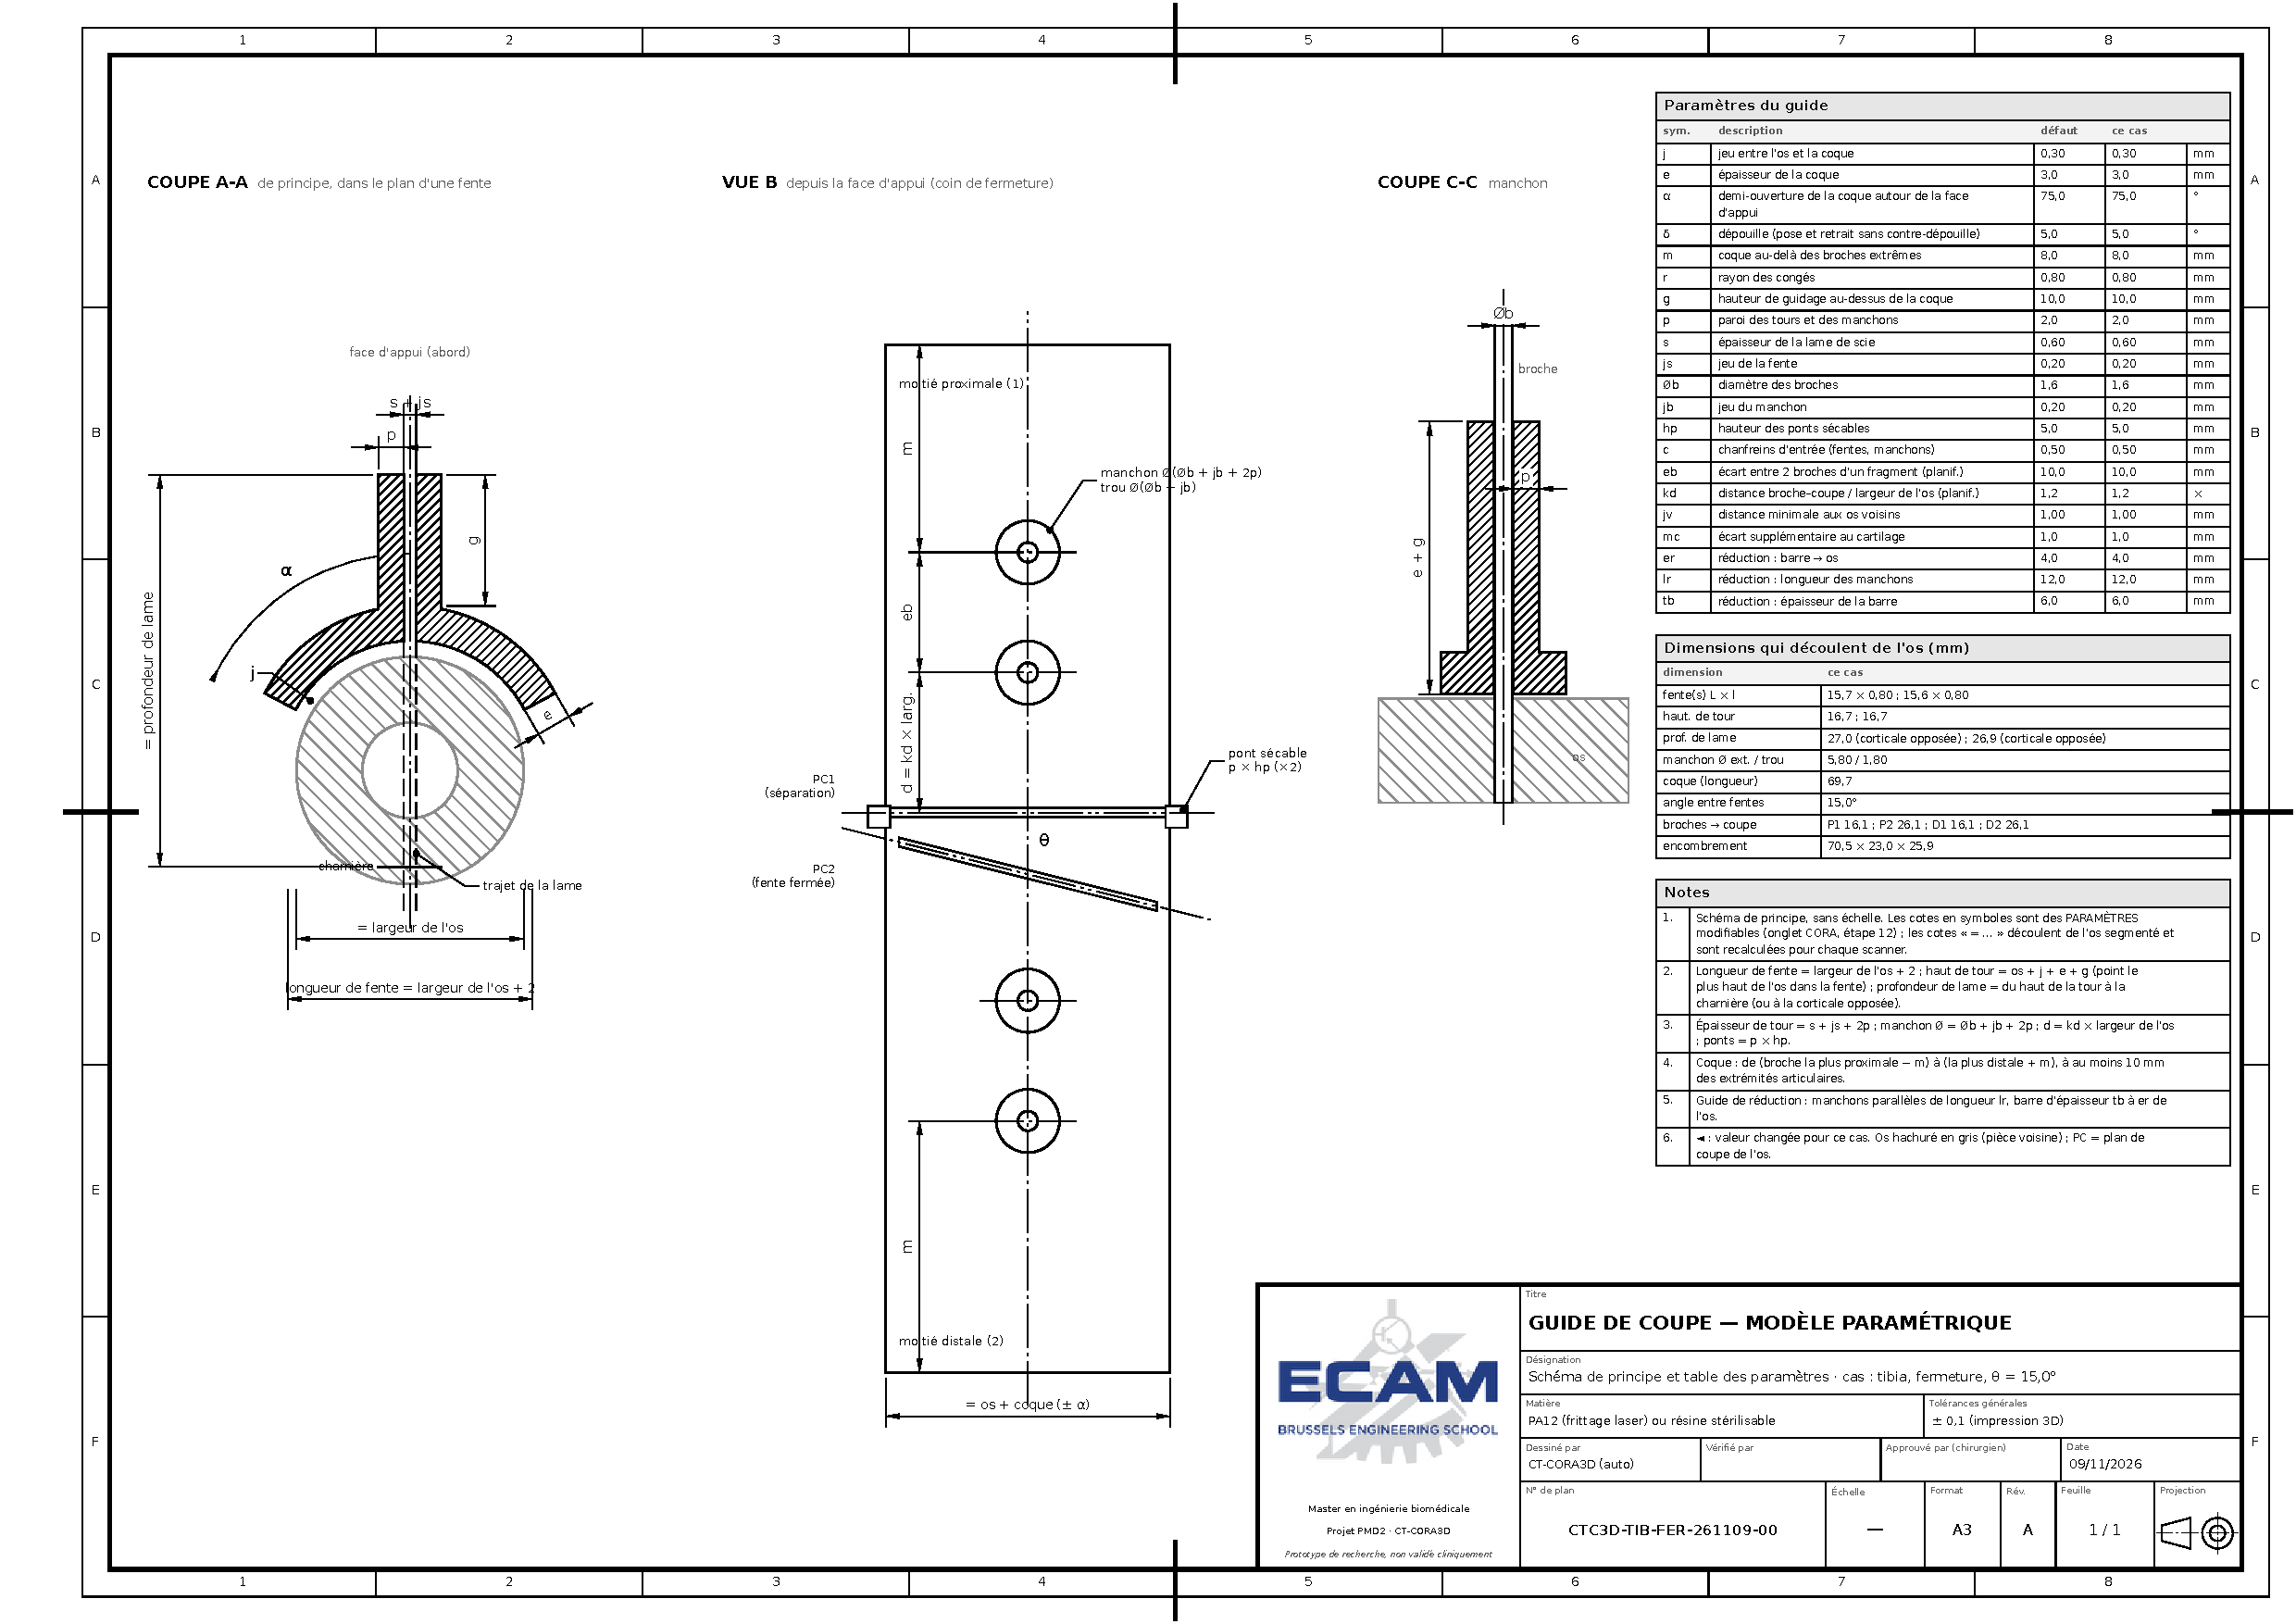
\includegraphics[width=\linewidth, height=0.9\textheight, keepaspectratio]{plan_generique.pdf}
\caption{Le plan générique du guide : le modèle paramétrique, avec ses cotes en symboles, le tableau des
paramètres et le cartouche (feuille A3 réduite ; le PDF est vectoriel, on peut zoomer).}
\label{fig:plan-generique}
\end{figure}
\begin{figure}[p]
\centering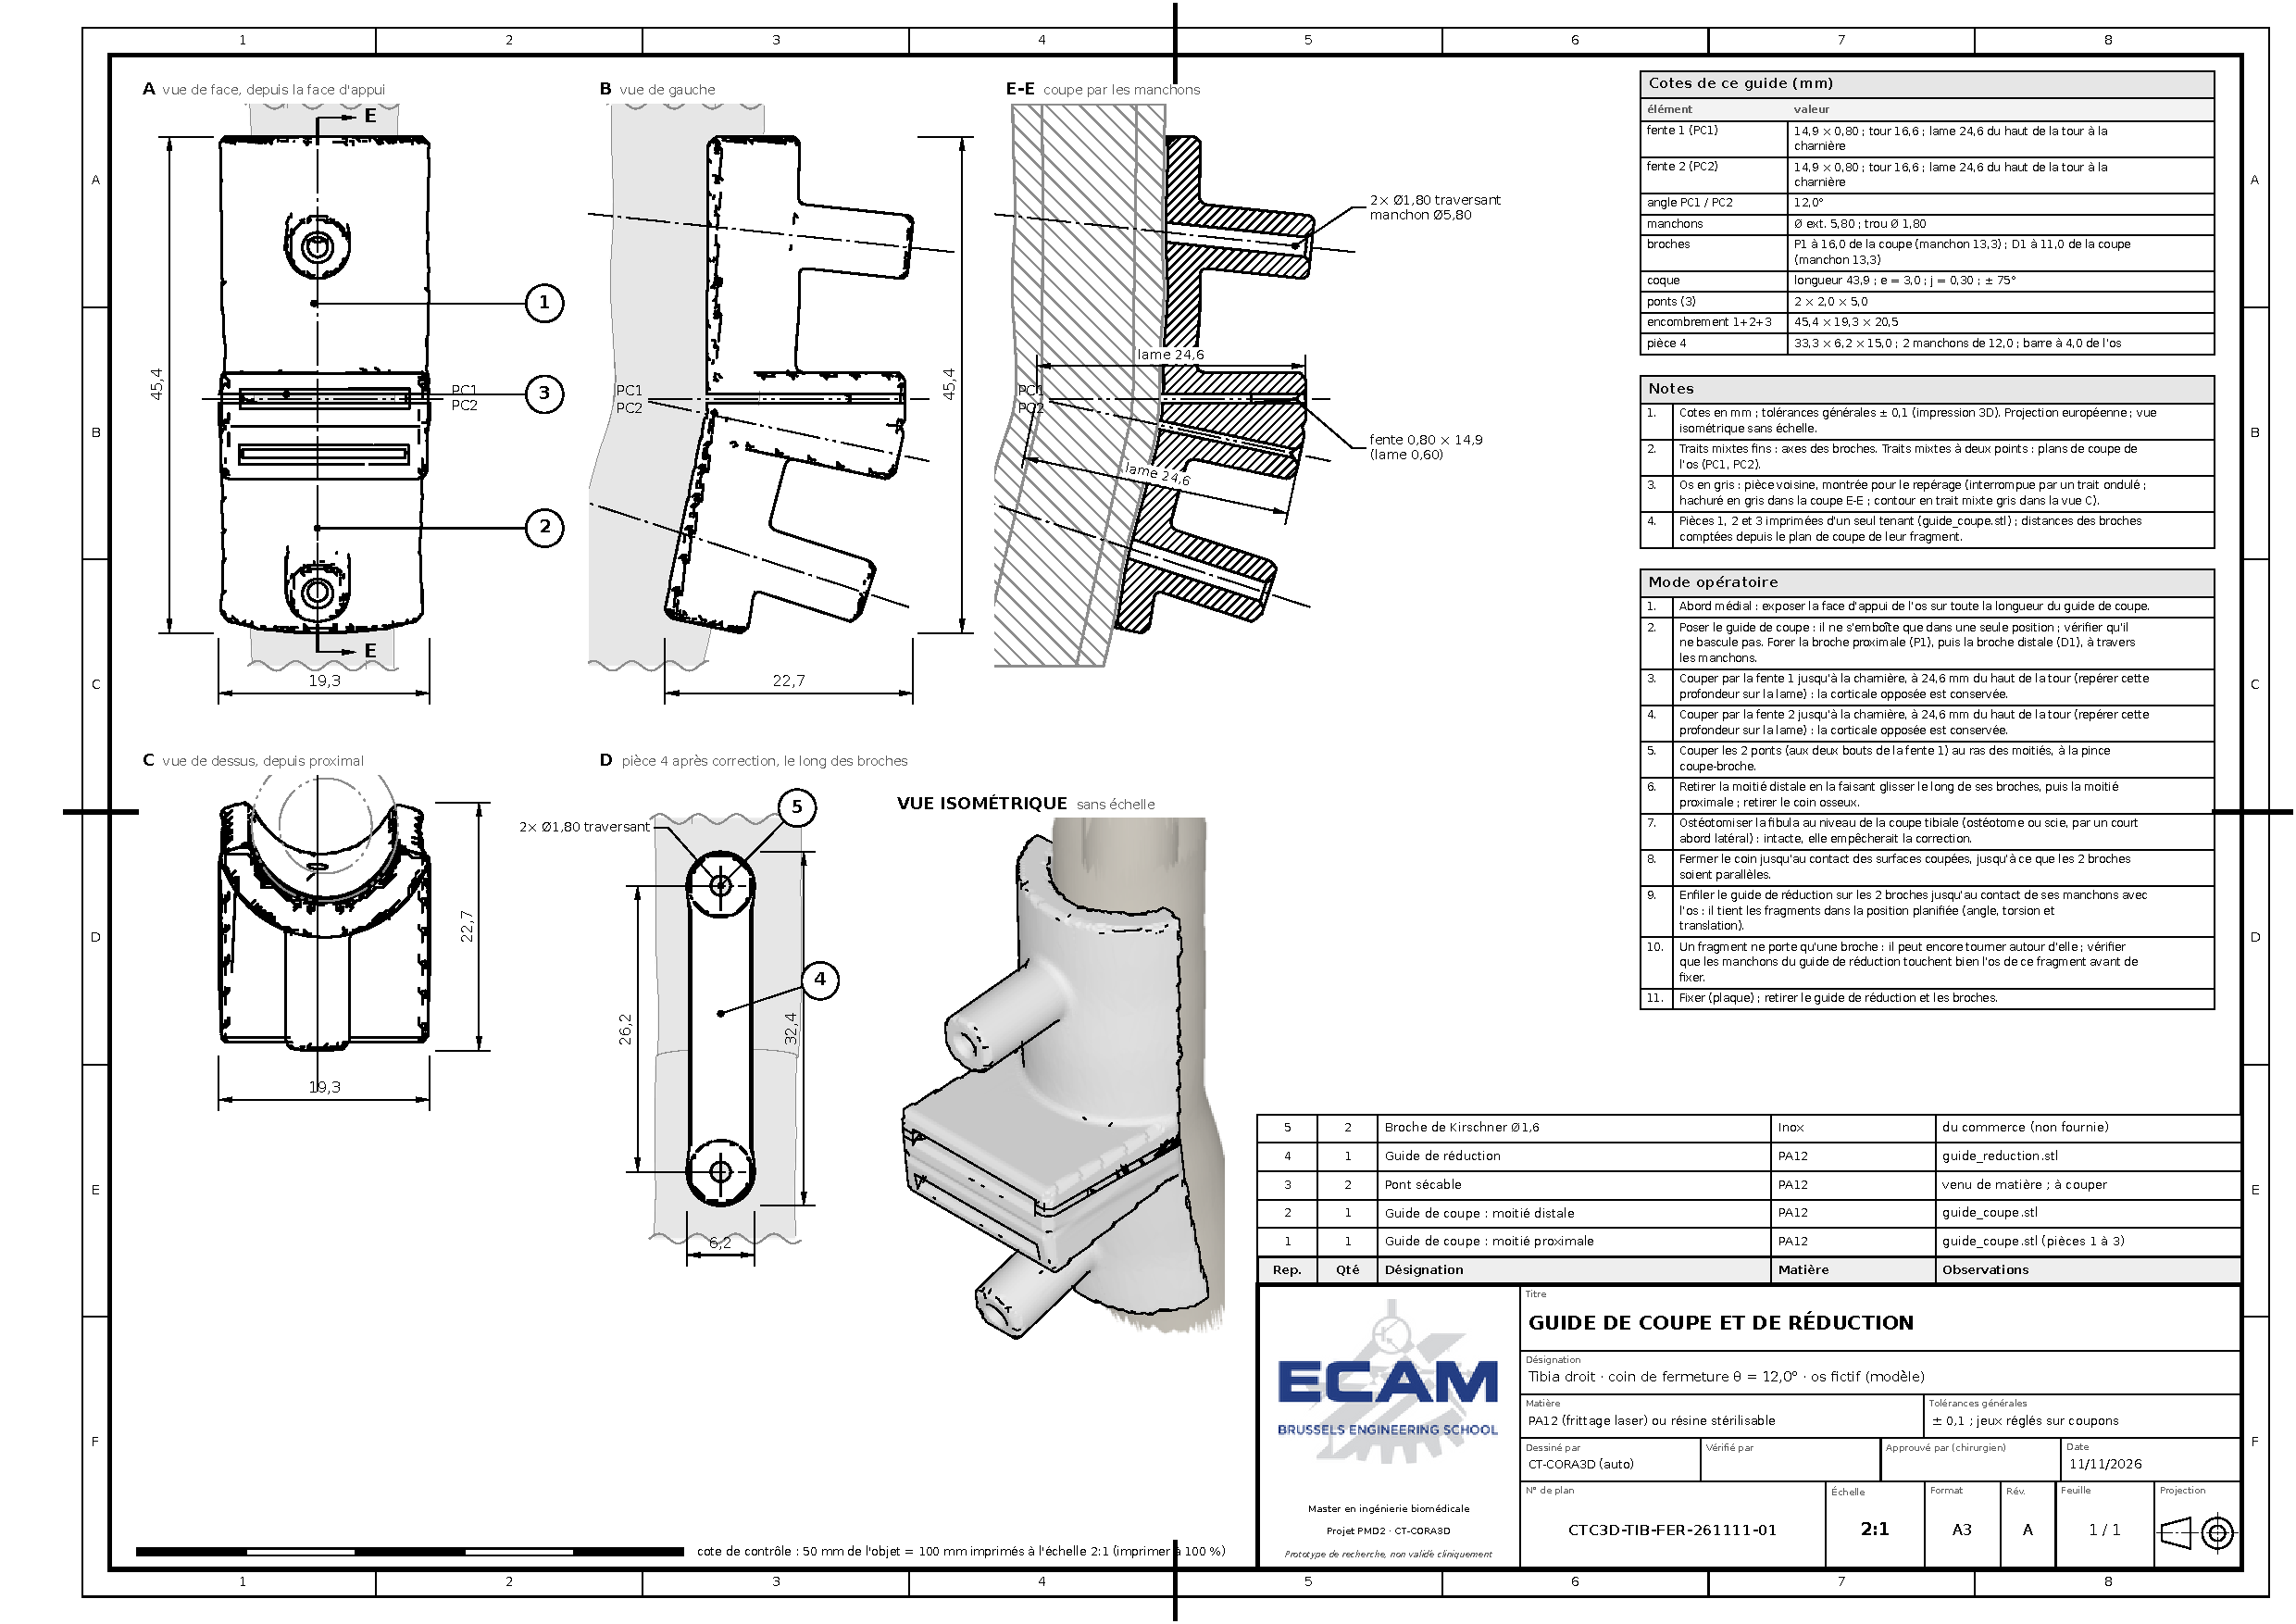
\includegraphics[width=\linewidth, height=0.9\textheight, keepaspectratio]{plan_guide.pdf}
\caption{Le plan coté produit automatiquement pour un guide de coin de fermeture du tibia : vues A, B et C,
coupe E-E, guide de réduction D, vue isométrique, nomenclature et cartouche (feuille A3 réduite).}
\label{fig:plan-guide}
\end{figure}
\end{landscape}
\pagestyle{fancy}


\partie{Le logiciel, les tests et la suite}{Comment les calculs deviennent une application de bureau, comment nous
avons vérifié les résultats, et ce qu'il reste à faire avant un usage clinique.}
\chapter{L'application}
\label{chap:application}

\begin{chapeau}
Ce chapitre explique comment les étapes de calcul deviennent une application de bureau : les couches du logiciel, le
serveur local, l'interface, la fenêtre, l'application autonome, comment la lancer sur Mac et sur Windows, et les
fichiers qu'elle produit.
\end{chapeau}

\section{Des étapes de calcul à une application}

Les fichiers \fichier{etape1} à \fichier{etape7} restent des modules Python ordinaires, utilisables en ligne de
commande. L'application ajoute trois couches autour d'eux, sans les réécrire (\cref{fig:architecture}) :
\begin{enumerate}
  \item un \textbf{serveur local} (\fichier{application/serveur.py}) qui importe les modules et les appelle à la
  demande ;
  \item une \textbf{interface web} (HTML et JavaScript) qui envoie les clics de l'utilisateur au serveur et affiche les
  résultats ;
  \item une \textbf{fenêtre native} (\fichier{application/fenetre.py}) qui affiche cette interface comme une vraie
  application, avec son nom et son icône.
\end{enumerate}
Enfin, \textbf{PyInstaller} peut emballer le tout dans un seul programme, avec Python et toutes les bibliothèques.

\fig{architecture_application.pdf}{L'organisation du logiciel : tout reste sur l'ordinateur.}{fig:architecture}

\section{Le serveur local}
\label{sec:serveur}

\subsection{Le principe}

Le serveur est un petit serveur web, construit avec le module \code{http.server} de Python. Il n'écoute que l'adresse
\code{127.0.0.1} : il n'est joignable que depuis l'ordinateur lui-même, et rien ne passe par Internet. Il choisit un
port libre au démarrage. Chaque bouton de l'interface correspond à une adresse (\cref{tab:api}).

\begin{table}[htbp]
\centering\small
\caption{Les principales adresses du serveur.}
\label{tab:api}
\begin{tabularx}{\linewidth}{L{4.2cm}Y}
\toprule
\titrecol{Adresse} & \titrecol{Rôle} \\
\midrule
\code{/api/action} & lance un calcul : \code{inventaire}, \code{ouvrir}, \code{segmenter}, \code{nommer},
\code{separer}, \code{oublier}, \code{guide} \\
\code{/api/etat} & donne l'avancement du calcul en cours (étape, journal, erreur, résultat) \\
\code{/api/serie}, \code{/api/coupe} & décrit la série ouverte ; renvoie une coupe du scanner en image, os colorés \\
\code{/api/point}, \code{/api/maillage} & valeur sous le curseur ; maillage 3D d'un os \\
\code{/api/cora/cas}, \code{/api/cora/os}, \code{/api/cora/maillage} & l'os à planifier, ses repères et son maillage dans le repère de l'os \\
\code{/api/cora/guide}, \code{/api/cora/guide/fichier} & le résultat de l'étape 7 et ses fichiers (affichage, téléchargement) \\
\code{/api/choisir_dossier}, \code{/api/montrer} & choisir un dossier de scanners ; ouvrir le dossier des résultats \\
\code{/api/quitter} & arrêter le serveur \\
\bottomrule
\end{tabularx}
\end{table}

\subsection{Un calcul à la fois, dans le fil principal}

Sur macOS, la bibliothèque VTK exige de tourner dans le fil principal du programme. Les calculs y sont donc exécutés,
un à la fois ; le serveur HTTP tourne à côté et ne fait que lire (coupes, maillages, fichiers). Quand l'utilisateur
clique sur \ui{Segmenter la série}, la demande est mise en file, le serveur répond tout de suite, et l'interface
interroge \code{/api/etat} plusieurs fois par seconde pour afficher l'avancement (\cref{fig:parcours}). Pendant un
calcul, le serveur empêche la mise en veille de l'ordinateur par inactivité.

\fig[0.72]{parcours_requete.pdf}{Le parcours d'une demande, du clic au résultat.}{fig:parcours}

Par exemple, la fonction \code{segmenter()} du serveur applique les réglages choisis dans l'interface (seuil, lissage)
aux paramètres de \fichier{parametres.py}, appelle \code{lancer_tout.traiter()}, c'est-à-dire \textbf{les mêmes étapes
1 à 6 qu'en ligne de commande}, puis remet les paramètres d'origine et garde le résultat en mémoire.

\section{L'interface}

\subsection{Onglet 1 · Segmentation CT}

La liste des séries trouvées, les coupes du scanner (axiale, coronale, sagittale) avec les os en couleur, les os en 3D
et la liste des os avec leur nom, leur volume et la raison de ce nom (\cref{fig:capture-segmentation}). On peut
\ui{Renommer} un os ou le \ui{Séparer} en cliquant des points. La carte \ui{Os à planifier (CORA)} propose l'os complet
de la série, avec un bouton \ui{Planifier CORA $\rightarrow$}.

\fig{capture_segmentation.png}{L'onglet \ui{Segmentation CT} avec une série segmentée : coupes du scanner, os en 3D et
liste des os trouvés.}{fig:capture-segmentation}

\subsection{Onglet 2 · Planification CORA}

Deux sources : l'\textbf{os segmenté} (celui de la série ouverte) ou l'\textbf{os fictif}. Un panneau à gauche permet
de choisir la référence (valeurs normales ou os avant déformité), une déformité de test, un des 17 préréglages
cliniques, la stratégie (type de coin, niveau du trait, profondeur de la charnière, broches) et les 27 dimensions du
guide. Au centre, la vue 3D (Three.js) ; à droite, le texte de l'étape en cours, parmi les 13 étapes
(\cref{tab:13etapes}). À l'étape 12, le bouton \ui{Construire les guides 3D} envoie la prescription au serveur, qui
lance l'étape 7.

\begin{pourquoi}
\textbf{Pourquoi un seul fichier HTML ?} Les modules JavaScript de \fichier{code_source/cora/app/} sont assemblés par
\fichier{code_source/cora/build_app.py} en un seul fichier, \fichier{application/interface/cora/index.html}, avec
Three.js, les polices et les données de l'os fictif. Il s'ouvre sans Internet et sans installation. En contrepartie,
il faut relancer \fichier{build_app.py} après chaque modification du JavaScript.
\end{pourquoi}

\subsection{La 3D à la demande}

Les vues 3D ne sont redessinées que quand quelque chose change (rotation, curseur, étape). Au repos, l'application ne
calcule aucune image : le processeur reste libre et l'ordinateur ne chauffe pas.

\section{La fenêtre native}

\fichier{application/fenetre.py} utilise la bibliothèque \textbf{pywebview}, qui affiche une page web dans une fenêtre
du système : le moteur WebKit (celui de Safari) sur macOS, WebView2 (celui d'Edge) sur Windows. L'application a ainsi
son nom et son icône dans le Dock ou la barre des tâches, des menus en français et des boîtes « Enregistrer sous » pour
les exports. Si pywebview ne peut pas être installé, l'application s'ouvre dans une fenêtre de Chrome ou d'Edge.

\section{L'application autonome}

Pour qu'un utilisateur n'ait rien à installer, PyInstaller copie Python, toutes les bibliothèques et le code dans une
application d'environ 800~Mo. Au lancement, un seul exécutable démarre \textbf{deux processus} : la fenêtre, et le
serveur de calcul (le même exécutable, lancé avec l'option \code{--serveur}). Sur macOS, la fenêtre (Cocoa) et les
calculs (VTK) exigent tous deux le fil principal : deux processus les séparent. Fermer la fenêtre arrête le serveur,
après le calcul en cours.

\begin{attention}
L'application autonome contient une \textbf{copie figée} du code : il faut la reconstruire après chaque modification
(\fichier{application/lanceurs/creer_app_autonome.sh} sur Mac, environ 3 minutes ;
\fichier{creer_app_windows.bat} sur Windows, environ 10 minutes la première fois).
\end{attention}

\section{Lancer le logiciel}
\label{sec:lancer}

\begin{table}[htbp]
\centering\small
\caption{Les façons de lancer CT-CORA3D.}
\label{tab:lancer}
\begin{tabularx}{\linewidth}{L{3.2cm}Y}
\toprule
\titrecol{Système} & \titrecol{Comment} \\
\midrule
macOS (conseillé) & \fichier{~/Applications/CT-CORA3D.app} : application autonome \\
macOS (développement) & \fichier{CT-CORA3D.app} du dossier du projet : petit lanceur qui utilise le Python de l'ordinateur \\
Windows (développement) & \fichier{Lancer sur Windows.bat} : essayé avec succès sur un PC Windows le 04/11/2026 \\
Windows (autonome) & raccourci créé par \fichier{application/lanceurs/creer_app_windows.bat} (recette écrite, pas encore construite) \\
\bottomrule
\end{tabularx}
\end{table}

Au premier lancement, les lanceurs de développement créent un environnement Python propre à l'ordinateur, hors de
OneDrive (\fichier{~/Library/Application Support/CTCORA3D/venv} sur Mac, \texttt{\%LOCALAPPDATA\%\textbackslash{}CTCORA3D\textbackslash{}venv} sur
Windows), y installent les bibliothèques (quelques minutes, Internet nécessaire), puis pywebview. Les lancements
suivants prennent quelques secondes : le lanceur vérifie seulement que les bibliothèques sont présentes, sans les
charger (0,02~s).

\subsection{Depuis GitHub}

Le code est versionné dans un dépôt GitHub \textbf{public} : chacun peut le récupérer
(\code{git clone}), installer Python 3.12 et lancer l'application comme ci-dessus. Les scanners DICOM ne sont pas dans le
dépôt (ils sont trop lourds) : il faut les placer dans le dossier \fichier{dicom/} de \fichier{CT-CORA3D/} (ou dans un
dossier \fichier{CT-scan/} à côté), ou les choisir par le bouton \ui{Changer de dossier…}. Un fichier \fichier{.gitattributes} impose les fins de ligne Windows aux fichiers
\fichier{.bat} : sans cela, un \fichier{.bat} récupéré depuis GitHub peut échouer sous Windows.

\section{Les fichiers produits}

\begin{table}[htbp]
\centering\small
\caption{Le contenu de \fichier{resultats/<série>/}.}
\label{tab:fichiers}
\begin{tabularx}{\linewidth}{L{4.6cm}Y}
\toprule
\titrecol{Fichier} & \titrecol{Contenu} \\
\midrule
\fichier{femur.stl}, \fichier{tibia.stl}\ldots & un maillage étanche par os, en millimètres, repère du scanner \\
\fichier{segmentation.seg.nrrd} & toutes les étiquettes, avec noms et couleurs (s'ouvre dans 3D Slicer) \\
\fichier{rapport.md}, \fichier{rapport.json} & le rapport de la segmentation \\
\fichier{apercu_3d.png}, \fichier{apercu_coupes.png} & des images de contrôle \\
\fichier{reperes_auto.mrk.json} & la tête du fémur, au format de 3D Slicer \\
\fichier{cora_<os>.json}, \fichier{.bin}, \fichier{.png} & repère, côté, repères, angles, torsion ; maillage dans le repère de l'os \\
\fichier{cora_cas.json} & l'os à planifier et la raison du choix \\
\fichier{guide_<os>_<coin>/} & \fichier{guide_coupe.stl} et \fichier{guide_reduction.stl} (à imprimer), \fichier{guide_coupe_scanner.stl}, \fichier{os_corrige.stl}, \fichier{prescription.json}, \fichier{guide.json} (contrôles, mode opératoire), plans 2D \\
\bottomrule
\end{tabularx}
\end{table}

Il n'y a pas de base de données : pour sauvegarder un cas, il suffit de copier son dossier. Le journal de
l'application est dans \fichier{~/Library/Logs/CTCORA3D.log} (Mac) ou \texttt{\%LOCALAPPDATA\%\textbackslash{}CTCORA3D\textbackslash{}CTCORA3D.log}
(Windows).

\section{Les performances}

\begin{table}[htbp]
\centering\small
\caption{Mesures sur le Mac de développement, avant et après le travail sur la fluidité (22/10/2026). Les résultats
des guides sont identiques au bit près.}
\label{tab:perf}
\begin{tabularx}{\linewidth}{Yrr}
\toprule
\titrecol{Mesure} & \titrecol{Avant} & \titrecol{Après} \\
\midrule
guide complet (tibia, fermeture, guide v3 avec verrou, plans 2D) & 86,5~s & 23,5~s \\
\quad dont plans 2D & 49,8~s & 6,2~s \\
chargement des bibliothèques du serveur & 2,1~s & 0,9~s \\
vérification de l'environnement par les lanceurs & 1,5 à 2,6~s & 0,02~s \\
vue 3D au repos (images calculées par seconde) & 60 & 0 \\
\bottomrule
\end{tabularx}
\end{table}

Les gains viennent de choix simples : plans 2D dessinés par un tampon de profondeur en numpy, recherches de voisins
sur tous les cœurs du processeur, et chargement des seules classes de VTK utilisées (\fichier{vtk_leger.py}). Depuis
la simplification du guide (06/11/2026), un guide complet avec ses plans prend 10 à 16~s.

\begin{danslecode}
\fichier{application/serveur.py} (serveur, actions, adresses), \fichier{application/fenetre.py} (fenêtre native),
\fichier{application/ct_cora3d_app.py} (point d'entrée de l'application autonome), \fichier{application/interface/}
(onglets), \fichier{application/lanceurs/} (fabrication des applications), \fichier{application/lancer_mac.sh} et
\fichier{Lancer sur Windows.bat} (lanceurs de développement).
\end{danslecode}

\chapter{Tests et validation}
\label{chap:validation}

\begin{chapeau}
Comment savoir si le logiciel donne le bon résultat ? Sans patient, nous avons testé sur des cas dont nous
connaissions la réponse : des déformités imposées à des os sains, un faux scanner de forme connue, et des campagnes de
centaines de cas contrôlés automatiquement. Ce chapitre présente la démarche et les résultats.
\end{chapeau}

\section{Trois niveaux de validation}

\fig{niveaux_validation.pdf}{Les trois niveaux de validation et leur état en novembre 2026.}{fig:niveaux}

Le niveau 1 vérifie que les calculs sont \textbf{justes} ; le niveau 2 qu'ils sont \textbf{robustes} ; le niveau 3, à
venir, qu'ils sont \textbf{utiles} au bloc opératoire. Les deux premiers niveaux ne disent rien de l'erreur finale
d'une vraie opération : elle viendra surtout des repères sur un os malade, de l'impression, de la pose du guide et du
geste du chirurgien.

\section{Les tests automatiques}

Le projet contient des tests qui se relancent en une commande (\cref{ann:commandes}).

\begin{table}[htbp]
\centering\small
\caption{Les tests automatiques du projet.}
\label{tab:tests}
\begin{tabularx}{\linewidth}{L{4.4cm}Y}
\toprule
\titrecol{Test} & \titrecol{Ce qu'il vérifie} \\
\midrule
\fichier{tests/test_chaine.py} & lecture et segmentation d'un faux scanner DICOM de forme connue : 14 contrôles (environ 3~s) \\
\fichier{tests/test_reperes.py} & repères sur l'os fictif posé au hasard et sur les os du lévrier : 40 contrôles (environ 13~s) \\
\fichier{tests/test_guide.py} & guides sur un os coudé synthétique (fermeture, ouverture avec dérotation, os voisin et cartilage) et sur les os du lévrier (environ 25~s) \\
\fichier{cora/tests/test_cas.mjs} & planification sur l'os fictif : 12 cas, 252 variantes et la torsion \\
\fichier{cora/tests/test_reel.mjs} & planification sur les os segmentés : tels quels, puis 6 déformités de test chacun \\
\fichier{tests/campagne_strategie.mjs} & 606 stratégies simulées, 9 règles \\
\fichier{tests/campagne_export.mjs} + \fichier{campagne_guides.py} & centaines de guides construits puis contrôlés « avec l'œil du chirurgien » \\
\bottomrule
\end{tabularx}
\end{table}

\subsection{Le faux scanner}

Le test \fichier{test_chaine.py} écrit en DICOM un fantôme dont on connaît tout : deux « os » en forme de capsule
(cylindre de 7~mm de rayon à bouts hémisphériques), bout à bout, séparés par un interligne de 1,5~mm et inclinés de
15\degre ; une corticale de 1,5~mm à 1300~HU, une moelle et des tissus mous à 40~HU, une table de scanner et un cylindre
de calibration ; un flou gaussien de 0,5~mm et un bruit de 40~HU. Les fichiers sont mélangés pour vérifier que le tri ne
dépend pas des noms. Le test vérifie la géométrie, la séparation des deux os, le rejet du fantôme de calibration,
l'étanchéité des maillages et la position de la surface (\cref{sec:demi-hauteur}).

\section{La segmentation}

\begin{itemize}
  \item \textbf{Position de la surface} (faux scanner) : biais de $+0{,}60$~mm avec le seul seuil, $+0{,}16$~mm après
  l'affinage à demi-hauteur ; objectif : moins de 0,5~mm.
  \item \textbf{Sensibilité au seuil} (lévrier, ± 50~HU) : 0,1 à 0,2~mm en moyenne, moins de 0,5~mm pour 95~\% des
  points (\cref{tab:sensibilite}).
  \item \textbf{Identification} : sur les trois scanners du lévrier, le fémur, le tibia, la fibula, la rotule, les
  fabelles, le talus, le calcanéus, le tarse, les métatarses, les phalanges et le bassin sont reconnus ; les maillages
  des os seuls sont étanches, de caractéristique d'Euler 2.
\end{itemize}

\section{Les repères}

Sur l'os fictif posé dans quatre positions au hasard (deux en miroir), le côté est reconnu 8 fois sur 8, les repères
sont à moins de 1~mm des repères exacts et identiques d'une pose à l'autre, et les angles de face diffèrent de moins de
1,3\degre{} de ceux du modèle. Sur le lévrier, les os coupés par le champ sont refusés et tous les angles des os
complets sont dans les normes (\cref{tab:normales-levrier}).

\section{La planification}

\begin{itemize}
  \item \textbf{Os fictif, 264 déformités} : l'angle de la déformité est retrouvé avec une erreur maximale de
  0,0065\degre.
  \item \textbf{Os du lévrier avec déformités de test} (référence : l'os avant la déformité) : erreur inférieure à
  0,001\degre ; après la correction simulée, les angles reviennent à ceux de l'os sain et une torsion de 15\degre{} est
  corrigée à 0,01\degre{} près ; les broches sont parallèles après la correction.
  \item \textbf{Référence « valeurs normales »} : l'écart naturel du lévrier à la moyenne publiée se retrouve dans la
  planification (plusieurs degrés). Ce n'est pas une erreur de calcul : quand c'est possible, il vaut mieux comparer au
  membre opposé du même chien.
\end{itemize}

\subsection{La campagne de stratégie}
\label{sec:campagne-strategie}

La campagne de stratégie (19/10/2026) planifie 606 cas : les 17 préréglages et leurs variantes (configurations de
broches, trait déplacé de ± 15~mm, charnière à 0,5 et 6~mm, chien en croissance) et 300 déformités tirées au hasard.
Pour chaque cas, les deux coins sont planifiés et contrôlés par 9 règles écrites à l'avance (\cref{tab:regles-r}).

\begin{table}[htbp]
\centering\small
\caption{Les 9 règles de la campagne de stratégie : 606 cas sur 606 sans erreur.}
\label{tab:regles-r}
\begin{tabularx}{\linewidth}{lYr}
\toprule
& \titrecol{Règle} & \titrecol{Erreurs} \\
\midrule
R1 & le guide n'est jamais du côté de la charnière & 0 \\
R2 & la charnière n'est dite conservée que si elle peut l'être (face du coin, règle 1, pas de dérotation, pont ≤ 3~mm) & 0 \\
R3 & la face d'appui est à 60\degre{} au plus de la face du coin, sinon l'abord non usuel est signalé & 0 \\
R4 & le coin recommandé est réalisable dès qu'un des deux l'est & 0 \\
R5 & le nombre et la disposition des broches sont ceux demandés & 0 \\
R6 & les broches sont parallèles après la correction & 0 \\
R7 & l'angle et la translation résiduels sont nuls & 0 \\
R8 & le niveau du trait et la profondeur de charnière demandés sont respectés & 0 \\
R9 & les angles après la correction sont ceux de l'os sain & 0 \\
\bottomrule
\end{tabularx}
\end{table}

Les coins recommandés suivent la pratique publiée : tibia en valgus → fermeture (84 cas) et tibia en varus → ouverture
(69 cas), avec l'accès comme critère décisif ; fémur → fermeture, avec la stabilité comme critère décisif.

\section{Les guides}

\subsection{La première campagne : un outil pour progresser}

La première campagne (14/10/2026) a construit et contrôlé des guides sur l'os fictif, avec ses os voisins et son
cartilage. Au début, seulement 46 cas sur 480 étaient sans erreur. Chaque type d'erreur a été corrigé dans le code, puis
la campagne a été relancée sur 640 cas, dont 320 tirés au hasard avec une graine jamais utilisée pendant le
développement : 640 sur 640 sans erreur (\cref{fig:campagne-guides}).

\fig{campagne_guides.png}{Les erreurs trouvées puis corrigées pendant la première campagne de guides.}{fig:campagne-guides}

Mesures après correction (minimum / médiane / maximum) : jeu guide--os 0,29 / 0,30 / 0,32~mm ; appui du guide 960 /
1470 / 2534~mm² ; guide à au moins 1~mm des os voisins et 1,5~mm du cartilage ; angles après la correction à
0,016\degre{} près ; broches parallèles à $2 \times 10^{-6}$ degré près.

\subsection{Les campagnes des guides v3 et du guide simplifié}

Après l'ajout d'une butée de profondeur, d'un verrou de réduction et de l'interdiction de l'espace entre les os, une
campagne (22/10/2026) a porté sur 520 cas : 320 cas « coins », où chaque paramètre est à ses valeurs extrêmes, et 200
cas tirés au hasard. Résultat : 520 sur 520 sans erreur. Le guide a ensuite été simplifié (06/11/2026, butée graduée
et verrou retirés, \cref{chap:guides}), et la même campagne a été relancée sur le nouveau guide : \textbf{520 sur 520
sans erreur} (\cref{tab:v3}).

\begin{table}[htbp]
\centering\small
\caption{La campagne du guide simplifié (06/11/2026). « Pas de guide » : coins que la planification déclare non
réalisables (elle conseille l'autre coin), construits quand même pour éprouver le programme ; le refus est le
comportement voulu.}
\label{tab:v3}
\begin{tabular}{lrr}
\toprule
& \titrecol{Coins (320)} & \titrecol{Hasard (200)} \\
\midrule
guide de coupe et guide de réduction construits & 266 & 159 \\
pas de guide : coin forcé, fibula sur le trajet de la lame & 54 & 41 \\
jeu guide--os mesuré & 0,296 à 0,327~mm & 0,298 à 0,324~mm \\
durée par guide (min / médiane / max) & 9 / 15 / 25~s & 10 / 15 / 23~s \\
\bottomrule
\end{tabular}
\end{table}

\subsection{Sur les os du lévrier}

Avec des déformités de test, les guides du fémur (coin de fermeture, torsion de test de 15\degre) et du tibia (coins de
fermeture et d'ouverture) sont construits sans alerte, avec un jeu de 0,31 à 0,33~mm, deux moitiés retirables et un
guide de réduction, en 10 à 16~s.

\section{La précision comparée}

\fig{precision.png}{L'erreur de notre calcul comparée à l'objectif du projet et aux résultats publiés.}{fig:precision}

L'erreur de calcul est si petite qu'elle ne se voit pas sur le graphique (\cref{fig:precision}). Les repères
automatiques (1,3\degre{} au plus de face sur l'os fictif) restent sous l'objectif de 2\degre. L'essentiel de l'erreur
d'une vraie opération viendra d'ailleurs.

\begin{aretenir}
\begin{itemize}
  \item Les calculs sont exacts à quelques millièmes de degré sur les cas simulés.
  \item Plus de 2 300 cas (stratégies et guides) passent tous les contrôles écrits à l'avance.
  \item Les campagnes ont surtout servi à \textbf{trouver des erreurs} : 434 cas sur 480 en avaient au départ.
  \item Rien n'a encore été imprimé ni essayé sur un os, et aucun vrai cas n'a été planifié : c'est le niveau 3.
\end{itemize}
\end{aretenir}

\chapter{Limites, sécurité et suite du projet}
\label{chap:limites}

\begin{chapeau}
Ce chapitre dit ce que le logiciel ne fait pas encore, ce qu'il faut surveiller avec les données, et ce qu'il reste à
faire. Il se termine par la conclusion du projet.
\end{chapeau}

\section{Les limites}

\begin{itemize}
  \item \textbf{Un seul chien, et il est sain.} Les déformités sont simulées. Un os très déformé, un implant, un cal
  vicieux ou un petit chien pourraient tromper la détection des repères. Les repères doivent toujours être vérifiés à
  l'écran (étape 1 de l'onglet CORA, ou \fichier{cora_<os>.png}).
  \item \textbf{Les angles de profil} reposent sur des lignes articulaires courtes (20 à 30~mm) : ils sont sensibles à
  quelques degrés.
  \item \textbf{Les valeurs normales} sont publiées surtout pour quelques races (Labrador, berger allemand, golden
  retriever, rottweiler) et mesurées sur radiographie ; pour le lévrier, seule la pente du plateau tibial a une
  référence propre. Le meilleur témoin reste le membre opposé.
  \item \textbf{Un seul apex}, et au fémur seulement les déformités distales (\cref{sec:hypotheses}).
  \item \textbf{Seulement des coupes planes} : pas d'ostéotomie en dôme (\cref{sec:dome}).
  \item \textbf{Les cartilages et les physes} d'un os segmenté sont approchés par des fractions de la longueur de l'os ;
  les os voisins ne sont évités que s'ils ont été segmentés.
  \item \textbf{Les voies d'abord et les marges} (cartilage 3 à 5~mm, os voisins 1 à 2~mm, entrée des broches à
  50\degre{} au plus\ldots) sont des choix raisonnés, à valider avec un chirurgien.
  \item \textbf{Les tissus mous et la plaque} ne sont pas modélisés : une broche peut gêner la plaque, et l'abord doit
  dégager toute la zone d'appui du guide.
  \item \textbf{Les guides n'ont pas été imprimés.} Les jeux de 0,2~mm des fentes et des manchons doivent être réglés
  sur de petites pièces de test (coupons) ; la tenue à la stérilisation reste à vérifier (matériau conseillé : polyamide
  PA12 fritté au laser, ou résine stérilisable).
  \item \textbf{L'application autonome Windows} n'a pas encore été construite ; le lanceur Windows de développement,
  lui, a été essayé.
\end{itemize}

\section{La sécurité et les données}
\label{sec:securite}

\begin{itemize}
  \item \textbf{Tout reste sur l'ordinateur.} Le serveur n'écoute que \code{127.0.0.1} et l'application n'envoie rien
  sur Internet.
  \item \textbf{Les en-têtes DICOM contiennent des noms.} Le nom de l'animal, parfois celui du propriétaire, et un
  identifiant sont recopiés dans \fichier{rapport.md}, \fichier{rapport.json} et le journal. Les résultats d'exemple du
  dépôt GitHub en contiennent : il faut les rendre anonymes avant de partager le dépôt plus largement (supprimer ces
  fichiers ne suffit pas, ils restent dans l'historique Git).
  \item \textbf{Le serveur ne vérifie pas l'origine des demandes.} Une page web ouverte sur le même ordinateur pourrait,
  en théorie, lui envoyer une commande. Il faudrait un jeton tiré au hasard au démarrage et un contrôle de l'origine.
  \item \textbf{OneDrive} copie le projet sur les serveurs de l'école : c'est acceptable pour les données d'exemple ;
  pour de vrais cas cliniques, il faut l'accord de l'établissement, ou un dossier non synchronisé.
  \item \textbf{Les fichiers à imprimer} (STL) ne contiennent que la forme des pièces, aucune donnée sur l'animal.
\end{itemize}

\begin{attention}[title={Un prototype de recherche}]
CT-CORA3D n'est pas un dispositif médical. Il ne doit pas servir sur un animal sans validation de chaque planification
par le chirurgien.
\end{attention}

\section{La suite du projet}

\begin{enumerate}
  \item \textbf{Imprimer et essayer.} D'abord des coupons de fentes et de manchons pour régler les jeux, puis des
  guides sur des os imprimés ; mesurer l'erreur finale (angle, torsion, translation) par scanner de l'os corrigé.
  \item \textbf{Vrais cas.} Obtenir les scanners complets de chiens opérés, rendus anonymes (\cref{sec:topogramme}), et
  comparer nos planifications à celles du chirurgien.
  \item \textbf{Robustesse.} D'autres scanners et d'autres races ; le membre opposé comme référence quand il est
  scanné ; des os vraiment déformés.
  \item \textbf{Nouvelles fonctions.} Une plaque sur mesure dont les trous de vis sont percés à travers le guide
  \cite{carwardine2021} ; les déformités à deux apex ; l'application autonome pour Windows.
  \item \textbf{Sécurité.} Jeton et contrôle d'origine sur le serveur ; ne plus recopier les noms dans les rapports ;
  signature de l'application avant de la diffuser.
\end{enumerate}

\section{Conclusion}

CT-CORA3D relie, dans une seule application, le scanner d'une patte de chien à un guide de coupe prêt à imprimer. Chaque
étape s'appuie sur une méthode publiée ou sur un calcul simple et vérifiable : la matrice DICOM, une segmentation par
seuil montant et croissance de région, des repères trouvés comme le ferait le chirurgien avec sa règle, la méthode CORA
de Paley faite en 3D, une stratégie choisie par des règles écrites, et un guide modélisé par des champs de distance puis
découpé par des opérations exactes. Sur des cas simulés, le calcul est exact à quelques millièmes de degré, et plus de
1\,800 cas passent tous les contrôles.

Les campagnes de simulation ont été l'outil le plus utile du projet : elles ont trouvé des centaines d'erreurs que
personne n'aurait vues sur un seul cas. Mais elles ont aussi montré leur limite : un guide « valide » sur le papier peut
être impossible à poser, et c'est le regard du chirurgien qui l'a révélé. La prochaine étape n'est donc plus seulement
informatique : il faut imprimer, essayer, et comparer avec le chirurgien sur de vrais patients.


\clearpage                       % la dernière page du chapitre 14 garde son onglet
\appendix
\annexetrue
\partieannexes{Le code fichier par fichier, tous les paramètres, le format de la prescription, un glossaire, les
commandes utiles et la bibliographie.}
\chapter{Le code, fichier par fichier}
\label{ann:code}

\begin{chapeau}
Cette annexe décrit chaque fichier du programme : son rôle, ses entrées, ses sorties et ses fonctions principales. Le
nombre de lignes est donné pour se faire une idée de la taille. Au total, le projet compte environ 10\,500 lignes de
Python et 6\,900 lignes de JavaScript et de HTML, dont environ 1\,900 lignes de tests et de campagnes.
\end{chapeau}

\newcommand{\fiche}[2]{\par\bigskip\noindent{\sffamily\bfseries\color{titre}\fichier{#1}}\hfill{\small\sffamily\color{gris}#2}\par\nopagebreak\smallskip}

\section{Arborescence}

\begin{lstlisting}[language={}, basicstyle=\ttfamily\footnotesize]
CT-CORA3D/
  CT-CORA3D.app            lanceur macOS de développement
  Lancer sur Windows.bat   lanceur Windows de développement
  LISEZ-MOI.md             mode d'emploi détaillé
  application/             serveur, fenêtre, interface, fabrication des applications
  code_source/             étapes 1 à 7 (Python), tests, cora/ (planification, JS)
  documents/               cahier des charges, rapport, documentation, ce dossier
  resultats/               un dossier par série, os fictif, rapports des campagnes
\end{lstlisting}

\section{Le programme de calcul : \texorpdfstring{\fichier{code_source/}}{code\_source/}}

\fiche{parametres.py}{198 lignes}
\textbf{Rôle} : tous les réglages du programme, au même endroit, chacun avec son origine (document de cadrage,
littérature ou mesure sur les scanners du projet). Aucune autre valeur « magique » ne doit apparaître dans les scripts.
Il définit aussi les dossiers : le dossier du projet, celui des scanners (\fichier{../CT-scan/} s'il existe) et celui
des résultats. Toutes les valeurs sont listées à l'\cref{ann:parametres}.

\fiche{etape1_lecture_dicom.py}{251 lignes}
\textbf{Rôle} : inventaire des séries d'un dossier et construction du volume (\cref{chap:lecture}).
\textbf{Entrée} : un dossier DICOM. \textbf{Sorties} : objets \code{Serie} et \code{Volume} (en mémoire).
\textbf{Fonctions} : \code{inventaire()} (fouille et regroupement par série), \code{charger()} (tri le long de la
normale, contrôles, rééchantillonnage, conversion en HU, matrice $\mt{A}$), \code{lire_pixels()},
\code{trouver()} (série par son nom) ; la classe \code{Volume} convertit indices et millimètres
(\code{vers_lps()}, \code{vers_indices()}).

\fiche{etape2_segmentation.py}{374 lignes}
\textbf{Rôle} : séparer les os (\cref{chap:segmentation}). \textbf{Entrée} : le \code{Volume}. \textbf{Sortie} :
un objet \code{Segmentation} (étiquettes, image lissée, géométrie de la zone recadrée).
\textbf{Fonctions} : \code{recadrage()}, \code{lisser()}, \code{graines_automatiques()} (seuil qui monte),
\code{croissance()} (ligne de partage des eaux), \code{contacts()}, \code{fusionner_surdecoupages()} (critère $c^*$),
\code{nettoyer()}, \code{segmenter()} (enchaîne le tout) ; outils de l'étape 3 : \code{recroissance()},
\code{raffiner()}, \code{boule()} ; \code{depuis_fichier()} relit une segmentation enregistrée ;
\code{boite_englobante()} calcule une boîte englobante 50 fois plus vite que la méthode classique.

\fiche{etape3_identification.py}{644 lignes}
\textbf{Rôle} : nommer les os et corriger la segmentation (\cref{chap:identification}). \textbf{Entrées} : la
\code{Segmentation}, les points de l'utilisateur. \textbf{Sorties} : noms, raisons, repère de la tête du fémur.
\textbf{Fonctions} : \code{decrire()} (descripteurs, ACP), \code{identifier()} (les 13 règles), \code{tete_femorale()}
et \code{ajuster_sphere()} (chapeau haut-de-forme et RANSAC), \code{separer_fibula()}, \code{separer_par_points()},
\code{nettoyer_morceaux()}, \code{nommer_cotes()}.

\fiche{etape4_maillage.py}{396 lignes}
\textbf{Rôle} : un STL étanche par os et la segmentation au format de 3D Slicer (\cref{chap:maillage}).
\textbf{Sorties} : \fichier{<os>.stl}, \fichier{segmentation.seg.nrrd}, les mesures de chaque maillage.
\textbf{Fonctions} : \code{exports()} (un fichier par os, plus le groupe « tarse »), \code{remplir()},
\code{mailler()}, \code{affiner_demi_hauteur()}, \code{controle()}, \code{bords_touches()}, \code{ecrire_stl()},
\code{ecrire_seg_nrrd()}, \code{lire_seg_nrrd()}, \code{exporter()}.

\fiche{etape5_controle.py}{267 lignes}
\textbf{Rôle} : sensibilité au seuil, aperçus et rapports (\cref{sec:sensibilite}). \textbf{Sorties} :
\fichier{rapport.md}, \fichier{rapport.json}, \fichier{apercu_3d.png}, \fichier{apercu_coupes.png},
\fichier{reperes_auto.mrk.json}. \textbf{Fonctions} : \code{sensibilite_seuil()}, \code{apercu_3d()},
\code{apercu_coupes()}, \code{markups()}, \code{rapport_md()}, \code{controler()}.

\fiche{etape6_reperes.py}{1236 lignes}
\textbf{Rôle} : repère, côté, complétude, repères anatomiques, angles et torsion du fémur et du tibia
(\cref{chap:reperes}). \textbf{Entrées} : les STL du dossier de résultats (et la fibula, la tête du fémur).
\textbf{Sorties} : \fichier{cora_<os>.json}, \fichier{cora_<os>.bin}, \fichier{cora_<os>.png}, \fichier{cora_cas.json}.
\textbf{Fonctions} : classe \code{Os} (repère courant, sections), \code{orienter()}, \code{cotes_femur()},
\code{cotes_tibia()}, \code{extremites_coupees()}, \code{analyser()} (les trois passes), \code{reperes_femur()},
\code{reperes_tibia()}, \code{tete_femorale()}, \code{centre_col()}, \code{petit_trochanter()},
\code{enveloppe_tangente()}, \code{sphere_robuste()}, \code{region_connexe()}, \code{angles_articulaires()},
\code{torsion()}, \code{calibration()}, \code{normales()}, \code{traiter_os()}, \code{choisir_cible()}. Ligne de
commande : \code{python etape6_reperes.py [dossiers] [--os tibia]}.

\fiche{etape7_guide.py}{2032 lignes}
\textbf{Rôle} : guide de coupe (deux moitiés reliées par des ponts sécables) et guide de réduction, avec leurs
contrôles (\cref{chap:guides}). \textbf{Entrées} : \fichier{prescription.json}, le maillage de l'os planifié, les os voisins et
le cartilage. \textbf{Sorties} : \fichier{guide_coupe.stl}, \fichier{guide_reduction.stl}, \fichier{guide_coupe_scanner.stl}, \fichier{os_corrige.stl},
\fichier{guide.json}, \fichier{guide.png}, les plans 2D, des \fichier{.bin} pour l'affichage.
\textbf{Fonctions} : \code{generer()}, \code{verifier_abord()}, \code{parametres_du_cas} (dimensions choisies pour un
cas), \code{Grille}, \code{distance_signee()}, \code{DistanceSurface}, \code{dist2_point_triangle()}, les champs
\code{champ_boite_arrondie()}, \code{champ_cylindre()}, \code{champ_capsule()}, \code{champ_secteur()}, \code{smin()},
\code{carte_hauteur()}, \code{depouille()}, \code{ombre()}, \code{EntreOs}, \code{sans_parties_fines()},
\code{isosurface()}, \code{guide_coupe()}, \code{transformation_reelle()}, \code{os_corrige()},
\code{guide_reduction()}, \code{controles_coupe()}, \code{controles_voisins()}, \code{controles_reduction()},
\code{protocole()},
\code{dimensions_guide()}, \code{assurer_jeu()}, \code{exporter()}.

\fiche{dessin_guide.py}{1230 lignes}
\textbf{Rôle} : les plans 2D du guide, générique (cotes en symboles) et coté (ce cas), en SVG, PDF et PNG, présentés
comme des plans de pièce industrielle (normes ISO). \textbf{Méthode} : projections orthogonales en projection
européenne, parties cachées par un tampon de profondeur en numpy, arêtes visibles en vecteurs ; coupe exacte
(manifold3d) hachurée ; cotes ISO, repères des pièces, nomenclature et cartouche avec le logo de l'ECAM
(\fichier{logo_ecam.png}) ; matplotlib, sans écran. \textbf{Fonctions} : \code{dessiner()}, \code{plan_generique()},
\code{plan_cote()}, \code{_rendu()} (tampon de profondeur), \code{_cote()}, \code{_hachures()},
\code{_cartouche()}, \code{_nomenclature()}.

\fiche{lancer_tout.py}{113 lignes}
\textbf{Rôle} : enchaîner les étapes 1 à 6 en ligne de commande, pour une série ou toutes. \textbf{Fonction} :
\code{traiter()}, appelée aussi par le serveur. Options : \code{--liste}, \code{--serie}, \code{--dossier},
\code{--sortie}, \code{--seuil}, \code{--ras}, \code{--sans-controle}, \code{--sans-images}.

\fiche{vtk_leger.py}{22 lignes}
\textbf{Rôle} : n'importer que les classes de VTK utilisées (0,5~s au lieu de 2,2~s au démarrage). Usage :
\code{import vtk_leger as vtk}.

\fiche{calibration_reperes.json}{fichier de données}
\textbf{Rôle} : cache des écarts de définition des angles (\cref{sec:calibration}), recalculé si
\fichier{etape6_reperes.py} change.

\section{Les tests : \texorpdfstring{\fichier{code_source/tests/}}{code\_source/tests/}}

\fiche{test_chaine.py}{172 lignes} Faux scanner écrit en DICOM, de géométrie connue ; contrôle de bout en bout des
étapes 1 à 5 (14 contrôles).

\fiche{test_reperes.py}{149 lignes} Os fictif dans des poses au hasard (repères exacts connus) et os du lévrier
(40 contrôles).

\fiche{test_guide.py}{378 lignes} Guides sur un os coudé synthétique (prescriptions écrites à la main) et sur les os du
lévrier ; option \code{--rapide}.

\fiche{modele_cora.py}{33 lignes} Lit l'os fictif (\fichier{cora/build/bones_pack.*}) depuis Python, pour les tests.

\fiche{campagne_export.mjs}{111 lignes} Génère les cas d'une campagne de guides (planification par le cœur
JavaScript, os, voisins et cartilage déformés).

\fiche{campagne_guides.py}{519 lignes} Construit les guides des cas en parallèle et les contrôle « avec l'œil du
chirurgien » ; écrit \fichier{rapport_campagne.md} et \fichier{resultats_campagne.jsonl}. Options \code{--processus},
\code{--filtre}, \code{--reprendre}, \code{--rapport}.

\fiche{campagne_strategie.mjs}{209 lignes} Campagne de la stratégie (préréglages et cas au hasard, règles R1 à R9) ;
option \code{--exporter} pour préparer une campagne de guides.

\section{La planification : \texorpdfstring{\fichier{code_source/cora/}}{code\_source/cora/}}

\fiche{app/cora_simple.js}{1727 lignes}
\textbf{Rôle} : le cœur de calcul de la planification, sans graphisme, utilisable sous Node (\cref{chap:planification}).
\textbf{Contenu} : vecteurs 2D et 3D, rotations (Rodrigues) et transformations rigides, réglages, préréglages
cliniques, paramètres du guide générique, valeurs publiées, \code{modeleReel()} (os segmenté au format du modèle),
\code{makeDeformity()}, \code{reference()}, \code{axesNormales()}, \code{coraPerpCommune()}, \code{planifier()},
\code{choisirAbord()}, \code{contraintesCoupe()}, \code{recommanderCoin()}, \code{placerBroches()},
\code{prescription()}, \code{mesuresTorsion()}, \code{planTorsion()}, \code{clipMesh()} (découpe de maillages),
\code{stlBinary()}.

\fiche{app/modules/10_base.js}{154 lignes} Utilitaires de l'interface (DOM, formatage), décodage du modèle osseux, et
la liste des références bibliographiques avec leurs DOI.

\fiche{app/modules/20_scene.js}{200 lignes} La scène 3D : rendu, caméra orthographique (comme une radiographie),
matériaux, et outils de dessin des tracés (lignes, points, arcs d'angle, plans, étiquettes).

\fiche{app/modules/30_os.js}{274 lignes} Les os dans la scène : os déformé, os sain en fantôme, fragments de
l'ostéotomie, broches, os tordu de l'étape « torsion ».

\fiche{app/modules/40_etapes.js}{1137 lignes} Les 13 étapes : titre, vue, légende et texte explicatif de chacune, avec
leurs chiffres et leurs sources.

\fiche{app/modules/45_export.js}{134 lignes} L'export pour le guide : archive ZIP (prescription, STL de l'os et des
voisins, carte du cartilage, mode d'emploi), écrite sans bibliothèque.

\fiche{app/modules/50_main.js}{1044 lignes} Le programme principal de l'onglet : état, panneaux, curseurs, sources (os
segmenté ou fictif), caméra, animation de la correction, construction des guides par le serveur, rendu à la demande
(\code{demanderImage()}).

\fiche{app/index.src.html}{401 lignes} Le gabarit de la page : structure et styles.

\fiche{build_app.py}{97 lignes} Assemble le gabarit, le cœur, les modules, Three.js, les polices et l'os fictif en un
seul fichier, \fichier{application/interface/cora/index.html}. À relancer après toute modification du JavaScript.

\fiche{generate_bones.py}{1149 lignes} Fabrique l'os fictif (fémur, tibia, fibula, rotule, fabelles d'un chien de
30~kg) par fonctions de distance et marching cubes, avec ses repères exacts et sa carte de cartilage ; écrit
\fichier{build/bones_pack.json} et \fichier{bones_pack.bin.gz}.

\fiche{tests/test_cas.mjs}{163 lignes} Planification sur l'os fictif : 12 cas, une grille d'amplitudes et de niveaux,
la torsion ; vérifie $\theta$, $F$, $S$, la formule de l'angle vrai, le CORA, la correction et les broches.

\fiche{tests/test_reel.mjs}{138 lignes} Planification sur les os segmentés, tels quels puis avec six déformités de test.

\section{L'application : \texorpdfstring{\fichier{application/}}{application/}}

\fiche{serveur.py}{1027 lignes} Le serveur local et les actions (inventaire, ouverture, segmentation, corrections,
guides) ; sert l'interface ; lance la fenêtre (\cref{sec:serveur}). Options : \code{--port}, \code{--sans-fenetre},
\code{--dossier}.

\fiche{fenetre.py}{288 lignes} La fenêtre native (pywebview) ; \code{--verifier} et \code{--installer} pour les
lanceurs.

\fiche{ct_cora3d_app.py}{80 lignes} Le point d'entrée de l'application autonome : sans option, la fenêtre ; avec
\code{--serveur}, le processus de calcul.

\fiche{interface/index.html}{130 lignes} La page à deux onglets (thème clair ou sombre, bouton Quitter).

\fiche{interface/ct/}{app.js 828, index.html 205 lignes} L'onglet \ui{Segmentation CT} : liste des séries, coupes,
os en 3D, corrections.

\fiche{interface/cora/index.html}{fichier produit} L'onglet \ui{Planification CORA}, assemblé par
\fichier{build_app.py}.

\fiche{lancer_mac.sh}{script} Choisit l'environnement Python (ou le crée au premier lancement) et lance le serveur ;
appelé par \fichier{CT-CORA3D.app}.

\fiche{lanceurs/}{scripts} \fichier{creer_app_autonome.sh} (application autonome macOS), \fichier{creer_app_mac.sh}
(petit lanceur \fichier{.app}), \fichier{creer_app_windows.bat} (application autonome Windows),
\fichier{ct_cora3d.spec} (recette PyInstaller commune), \fichier{lanceur_mac.applescript}.

\fiche{icone/creer_icone.py}{68 lignes} Dessine l'icône (coupe de scanner, fémur, axes et CORA) aux formats PNG, ICNS
et ICO.

\fiche{requirements.txt}{liste} Les bibliothèques Python : numpy, scipy, pydicom, SimpleITK, vtk, trimesh, pyvista,
matplotlib, pillow, manifold3d.

\section{Les documents : \texorpdfstring{\fichier{documents/}}{documents/}}

Le cahier des charges, le rapport de projet et la documentation technique (PDF et Word), leurs sources Markdown et
leurs figures, et ce dossier complet (\fichier{documents/dossier_complet/} : sources LaTeX, scripts des figures et
schémas draw.io modifiables).

\chapter{Tous les paramètres}
\label{ann:parametres}

\begin{chapeau}
Les réglages du programme sont tous dans \fichier{code_source/parametres.py}, chacun avec son origine. Les dimensions
du guide peuvent en plus être changées pour un cas dans l'application (panneau \ui{Guide générique : dimensions}),
dans les bornes indiquées ; une valeur changée est signalée dans \fichier{guide.json}.
\end{chapeau}

\section{Segmentation et maillage (étapes 1 à 5)}

{\footnotesize\renewcommand{\arraystretch}{1.2}
\begin{longtable}{L{6.5cm}rL{6.1cm}}
\toprule
\titrecol{Paramètre} & \titrecol{Valeur} & \titrecol{Signification et origine} \\
\midrule
\endhead
\code{EPAISSEUR_MAX_MM} & 1,0~mm & coupes plus épaisses : avertissement (document de cadrage) \\
\code{TOLERANCE_ESPACEMENT} & 5~\% & écart toléré entre deux intervalles de coupes \\
\code{TOLERANCE_ORIENTATION} & $10^{-3}$ & orientations identiques à $10^{-3}$ près \\
\code{SIGMA_LISSAGE_MM} & 0,35~mm & flou gaussien avant seuillage (bruit divisé par deux) \\
\code{SEUIL_OS_HU} & 226~HU & masque osseux (seuil « Bone (CT) » de Mimics) \\
\code{MARGE_RECADRAGE_MM} & 6~mm & marge autour des os denses \\
\code{SEUIL_GRAINE_DEPART_HU} & 500~HU & premier palier du seuil qui monte \\
\code{SEUIL_GRAINE_MAX_HU} & 1500~HU & dernier palier \\
\code{PAS_SEUIL_HU} & 100~HU & pas entre deux paliers \\
\code{VOLUME_MIN_MORCEAU_MM3} & 300~mm³ & taille minimale d'un morceau pour devenir une graine \\
\code{PERSISTANCE_HU} & 200~HU & le morceau doit exister encore 200~HU plus haut\ldots \\
\code{VOLUME_PERSISTANCE_MM3} & 50~mm³ & \ldots avec au moins ce volume \\
\code{VOLUME_MIN_GRAINE_MM3} & 30~mm³ & bloc dense plus petit : pas de graine \\
\code{VOLUME_MIN_SEGMENT_MM3} & 50~mm³ & segment plus petit : rattaché à son voisin \\
\code{RAPPORT_CONTACT_FUSION} & 3 & seuil du critère $c^*$ (coupure ≈ 5, articulation ≤ 2,1) \\
\code{LONGUEUR_OS_LONG_MM}, \code{ALLONGEMENT_OS_LONG} & 50~mm, 3 & définition d'un os long \\
\code{ALLONGEMENT_COMPACT} & 3,5 & os compact (rotule, tarse) \\
\code{VOLUME_MIN_NOMME_MM3} & 200~mm³ & en dessous, jamais nommé automatiquement \\
\code{CV_MAX_OBJET}, \code{FRACTION_SPONGIEUX_MAX_OBJET} & 0,2, 8~\% & objet non osseux : homogène, sans os spongieux \\
\code{CAVITE_MAX_OBJET} & 5~\% & \ldots et sans cavité \\
\code{RAYON_VALLEE_MM}, \code{PROFONDEUR_VALLEE_HU} & 1~mm, 250~HU & chapeau haut-de-forme de la hanche \\
\code{HU_MIN_VALLEE} & 150~HU & écarte les cloisons graisseuses \\
\code{RAYON_RECHERCHE_TETE_MM} & 35~mm & recherche autour du contact fémur--bassin \\
\code{RAYON_TETE_MM} & 4 à 20~mm & rayon plausible d'une tête de fémur \\
\code{TOLERANCE_SPHERE_MM} & 0,6~mm & distance d'un inlier à la sphère \\
\code{COUVERTURE_MIN_SPHERE}, \code{INLIERS_MIN_SPHERE} & 40~\%, 150 & validation de la sphère (lévrier : 68~\%, 2055) \\
\code{MARGE_SPHERE_MM} & 1~mm & graines fémur et bassin de part et d'autre de la sphère \\
\code{FRACTION_MAX_SESAMOIDE}, \code{CSTAR_MAX_SESAMOIDE} & 5~\%, 1,5 & fabelles détachées du fémur \\
\code{PAS_TRANCHES_MM} & 2~mm & tranches pour trouver la fibula \\
\code{AIRE_MIN_FIBULA_MM2}, \code{RAPPORT_AIRE_FIBULA_MAX} & 3~mm², 0,2 & petite tache de la fibula \\
\code{SERIE_MIN_FIBULA}, \code{SAUT_MAX_FIBULA_MM} & 15~\%, 3~mm & suivi de la tache d'une tranche à l'autre \\
\code{RAYON_GRAINE_MM} & 2,5~mm & boule autour d'un point de l'utilisateur \\
\code{RAYON_FERMETURE_MM} & 1~mm & fermeture avant remplissage \\
\code{SIGMA_MAILLAGE_MM} & 0,3~mm & flou du masque avant marching cubes \\
\code{ITERATIONS_LISSAGE}, \code{BANDE_PASSANTE_LISSAGE} & 20, 0,05 & lissage à fenêtre sinc \\
\code{TRIANGLES_MAX}, \code{REDUCTION_MAX} & 150\,000, 75~\% & décimation \\
\code{AFFINAGE_DEMI_HAUTEUR} & oui & affinage du bord à demi-hauteur \\
\code{PROFIL_INTERIEUR_MM}, \code{PROFIL_EXTERIEUR_MM} & 2,5, 2~mm & étendue du profil le long de la normale \\
\code{CONTRASTE_MIN_HU}, \code{DEPLACEMENT_MAX_MM} & 300~HU, 1,5~mm & validité de l'affinage \\
\code{LISSAGE_DEPLACEMENT} & 5 & passes de lissage des déplacements \\
\code{SYSTEME_COORDONNEES} & LPS & repère des STL (comme 3D Slicer) \\
\code{VARIATION_SEUIL_HU}, \code{ECART_SURFACE_CIBLE_MM} & 50~HU, 0,5~mm & contrôle de sensibilité au seuil \\
\code{CORA_COUVERCLE_MIN_MM2} & 80~mm² & couvercle plan : extrémité coupée par le champ \\
\bottomrule
\end{longtable}
}

\section{Le guide générique (étape 7)}

{\small\renewcommand{\arraystretch}{1.2}
\begin{longtable}{lL{6.4cm}rr}
\toprule
\titrecol{Symbole} & \titrecol{Dimension} & \titrecol{Défaut} & \titrecol{Bornes} \\
\midrule
\endhead
$j$ & jeu entre l'os et la coque & 0,3~mm & 0,1 à 1 \\
$e$ & épaisseur de la coque & 3~mm & 1,5 à 6 \\
$\alpha$ & demi-ouverture de la coque autour de la face d'appui & 75\degre & 30 à 120 \\
$m$ & coque au-delà des broches extrêmes & 8~mm & 3 à 25 \\
$\delta$ & dépouille (pose et retrait sans contre-dépouille) & 5\degre & 1 à 15 \\
$r$ & rayon des congés & 0,8~mm & 0 à 2 \\
$e_{\min}$ & épaisseur minimale imprimable & 1,2~mm & 0,6 à 3 \\
$g$ & hauteur de guidage au-dessus de la coque & 10~mm & 4 à 25 \\
$p$ & paroi des tours et des manchons & 2~mm & 1,2 à 4 \\
$s$ & épaisseur de la lame de scie & 0,6~mm & 0,3 à 1,5 \\
$j_s$ & jeu de la fente & 0,2~mm & 0,05 à 0,6 \\
$\varnothing_b$ & diamètre des broches & 1,6~mm & 1 à 3,2 \\
$j_b$ & jeu du manchon & 0,2~mm & 0,05 à 0,6 \\
$h_p$ & hauteur des ponts sécables & 5~mm & 2 à 10 \\
$c$ & chanfreins d'entrée & 0,5~mm & 0 à 1,5 \\
$k_d$ & distance broche--coupe préférée (× largeur de l'os) & 1,2 & 0,5 à 3 \\
$j_v$ & distance minimale aux os voisins & 1~mm & 0,5 à 4 \\
$m_c$ & écart supplémentaire de la coque au cartilage & 1~mm & 0,5 à 5 \\
$e_r$ & guide de réduction : distance de la barre à l'os & 4~mm & 2 à 15 \\
$l_r$ & guide de réduction : longueur des manchons & 12~mm & 6 à 25 \\
$t_b$ & guide de réduction : épaisseur de la barre & 6~mm & 3 à 12 \\
\bottomrule
\end{longtable}
}

\section{Autres réglages de l'étape 7}

\begin{itemize}
  \item \code{GUIDE_PAS_MM} = 0,3~mm : pas de la grille ; \code{GRILLE_MAX_NOEUDS} = 12 millions (au-delà, le pas
  grandit) ;
  \item \code{DISTANCE_MIN_ARTICULATION_MM} = 10~mm : la coque et les broches restent loin des extrémités de l'os ;
  \item \code{DENSITE_IMPRESSION_G_CM3} = 1,01 : polyamide PA12, pour estimer la masse des pièces ;
  \item dans \fichier{etape7_guide.py} : \code{COMPENSATION_MM} = 0,04~mm, \code{FROTTEMENT_MM3} = 0,5~mm³,
  \code{TOL_OMBRE_MM} = 0,5~mm.
\end{itemize}

\enlargethispage{2\baselineskip}      % la fin de la liste tient sur cette page
\section{Réglages de la planification (\texorpdfstring{\fichier{cora_simple.js}}{cora\_simple.js})}

\begin{itemize}[itemsep=0pt]
  \item \code{CHARNIERE_RETRAIT} = 2~mm, \code{PONT_MAX} = 3~mm, \code{CHARNIERE_OUVERTURE_MAX} = 3~mm ;
  \item \code{THETA_MIN} = 0,5\degre{} (en dessous, pas de CORA) ; \code{DEROTATION_MIN} = 1\degre ;
  \item \code{MARGE_COUPE_CARTILAGE} = 5~mm, \code{MARGE_BROCHE_CARTILAGE} = 3~mm, \code{MARGE_BROCHE_VOISIN} = 2~mm ;
  \item \code{ANGLE_ENTREE_MAX} = 50\degre{} (entrée d'une broche), \code{ANGLE_ENTREE_COIN_MAX} = 60\degre{} (face
  d'appui) ;
  \item \code{FRAGMENT_MIN_MM} = 25~mm, \code{MARGE_TUBEROSITE_MM} = 8~mm, \code{MARGE_EPICONDYLE_MM} = 6~mm ;
  \code{OUVERTURE_MAX_FRAC} = 40~\% de la largeur de l'os ; \code{RETRAIT_DERIVE_MAX} = 0,03.
\end{itemize}

\chapter{Le format de la prescription}
\label{ann:prescription}

\begin{chapeau}
La prescription (\fichier{prescription.json}, format v2.2) est le fichier qui relie la planification (JavaScript) à la
construction des guides (Python). Elle est écrite par la fonction \code{prescription()} de \fichier{cora_simple.js}.
Toutes les coordonnées sont en millimètres, dans le repère de l'os ($X$ latéral, $Y$ proximal, $Z$ caudal ; un membre
gauche y est mis en miroir). Les signes suivent la convention du prototype précédent : frontal $+$ = varus, sagittal
$+$ = procurvatum.
\end{chapeau}

\begin{table}[htbp]
\centering\small
\caption{Les blocs de la prescription.}
\label{tab:prescription}
\begin{tabularx}{\linewidth}{L{3.6cm}Y}
\toprule
\titrecol{Clé} & \titrecol{Contenu} \\
\midrule
\code{schema_version}, \code{os}, \code{cote}, \code{repere} & version du format, os, côté traité (toujours droit), description du repère \\
\code{deformite} & angle vrai, composantes frontale et sagittale, orientation $\varphi$, torsion mesurée, écart entre les axes $\delta$, position du CORA \\
\code{reference} & la référence utilisée : os sain, ou valeurs normales (avec leurs valeurs) \\
\code{strategie} & type de coin, règle de Paley, torsion corrigée ou non, niveau de coupe, translation, abord, face du coin, abord non usuel, os voisin sur la lame, profondeur de charnière, coin mixte, configuration des broches, recommandation et critère décisif, ostéotomie complète \\
\code{charniere} & point, direction, distance au CORA, profondeur, point de l'ACA (règle 2) \\
\code{plans_coupe} & pour chaque trait : un point, la normale, la profondeur (\code{charniere} ou \code{complete}) \\
\code{coin} & angle, base, profondeur de coupe, changement de longueur, rayons convexe et concave, angle entre les coupes, orientation de la charnière \\
\code{correction} & axe, angle, point, dérotation et son axe, matrices $4\times4$ de la correction complète et de la seule correction angulaire \\
\code{broches}, \code{broches_reduction} & pour chaque broche : fragment, point de l'axe, direction, diamètre, hauteur du manchon \\
\code{placement_broches} & rotation $\beta$, inclinaison $\gamma$, distances à la coupe, disposition, écarts, contraintes respectées \\
\code{guide_reduction} & position des broches après la correction \\
\code{torsion} & définition, valeurs avant, après correction angulaire, cible, après, dérotation, normale et seuils \\
\code{guide} & face d'appui, axes proximal et distal, centre de la section \\
\code{contraintes_coupe}, \code{alertes} & contraintes chirurgicales au niveau du trait (niveau, texte) ; alertes de la planification \\
\code{prevision} & angle et translation résiduels prévus (doivent être nuls) \\
\code{os_segmente} & os segmenté : série, fichier STL, côté anatomique, miroir, matrice os → scanner \\
\code{verite_terrain} & déformité de test : apex, angle, torsion imposés (pour la validation) \\
\code{parametres_guide} & dimensions du guide changées pour ce cas \\
\bottomrule
\end{tabularx}
\end{table}

\section*{Un extrait}

Extrait de la prescription du guide de la \cref{fig:guide-v3}, image d (os fictif, tibia, cas de démonstration d'un
grand varus
avec recurvatum, en coin de fermeture forcé ; valeurs arrondies, listes raccourcies) :

\begin{lstlisting}[language={}, basicstyle=\ttfamily\footnotesize]
{ "schema_version": "v2.2", "os": "tibia", "cote": "droit",
  "deformite":  { "theta_deg": 30.77, "frontal_deg": 28.02, "sagittal_deg": -15.04, "phi_deg": 26.79,
                  "ecart_axes_mm": 0.0008, "cora": [-0.05, 71.65, 0.84] },
  "strategie":  { "type_coin": "fermeture", "regle_paley": 1, "charniere_profondeur_mm": 2,
                  "abord_non_usuel": true, "configuration_broches": "1+1", "osteotomie_complete": true,
                  "recommandation": { "type_coin": "ouverture", "critere_decisif": "abord" } },
  "charniere":  { "point": [-3.57, 72.99, -2.79], "direction": [0.451, 0.004, -0.893] },
  "plans_coupe": [ { "point": [-3.57, 72.99, -2.79], "normale": [0.000, -1.000, -0.005], "profondeur": "complete" },
                   { "point": [-3.57, 72.99, -2.79], "normale": [-0.457, -0.858, -0.235], "profondeur": "complete" } ],
  "coin":       { "angle_deg": 30.77, "largeur_base_mm": 6.33, "profondeur_coupe_mm": 11.51, "delta_L_mm": -2.42 },
  "correction": { "axe": [-0.451, -0.004, 0.893], "angle_deg": 30.77, "derotation_deg": 0,
                  "T_4x4": [[0.888, -0.456, -0.059, 32.74], [0.457, 0.859, 0.230, 12.55],
                            [-0.055, -0.231, 0.971, 16.60], [0, 0, 0, 1]] },
  "broches_reduction": [ { "fragment": "proximal", "point_axe": [-0.94, 86.16, 2.69],
                           "direction": [-0.860, 0.268, -0.434], "diametre_mm": 1.6, "hauteur_manchon_mm": 15 }, ... ],
  "prevision":  { "angle_residuel_deg": 0, "translation_residuelle_mm": 0.0008 } }
\end{lstlisting}

\enlargethispage{3\baselineskip}%
On y vérifie quelques relations du \cref{chap:planification} : les deux plans de coupe passent par la charnière ;
leurs normales font l'angle $\theta = 30{,}8\degre$ ; la direction de la charnière est l'axe de correction (au signe
près) ; la base vaut $2 D \tan(\theta/2)$ avec $D = 11{,}5$~mm, soit 6,3~mm ; la planification conseillait le coin
d'ouverture (critère : l'accès), et ce coin de fermeture a été forcé pour éprouver le programme.

\chapter{Glossaire}
\label{ann:glossaire}

\begin{description}[style=nextline, leftmargin=1.2em, font=\sffamily\bfseries\color{titre}, itemsep=0.25em]
  \item[Abord (voie d'abord)] Chemin par lequel le chirurgien atteint l'os, à travers la peau et les muscles.
  \item[ACA] \emph{Angulation correction axis} : axe autour duquel on fait tourner le fragment distal pour corriger
  l'angle. Il doit être sur la bissectrice transverse du CORA.
  \item[ACP (analyse en composantes principales)] Calcul des directions dans lesquelles un nuage de points est le plus
  étendu.
  \item[Angle vrai] Angle de la déformité mesuré en 3D, dans son plan ; il n'est pas la somme des angles vus de face et
  de profil.
  \item[Antéversion] Torsion du fémur : angle entre l'axe du col et la ligne qui passe derrière les condyles.
  \item[Apex] Sommet de la courbure d'un os déformé.
  \item[Axe anatomique, axe mécanique] Axe qui suit le milieu de la diaphyse ; axe qui relie les centres des deux
  articulations.
  \item[Bissectrice transverse] Droite qui partage en deux l'angle entre les axes des deux segments, dans le plan de la
  déformité.
  \item[Broche de Kirschner] Fine tige métallique forée dans l'os (ici 1,6~mm).
  \item[Charnière] Petit pont d'os laissé intact, autour duquel les fragments tournent.
  \item[Coin de fermeture, d'ouverture] Correction qui retire un coin d'os (deux traits) ; correction qui ouvre l'os
  (un trait).
  \item[Contre-dépouille] Partie d'une pièce qui passe « sous » l'objet et empêche de la poser ou de la retirer en
  translation.
  \item[CORA] \emph{Center of rotation of angulation} : point où se croisent les axes des deux segments d'un os
  déformé.
  \item[Corticale] Couche d'os dense qui forme le tube de la diaphyse.
  \item[Croissance de région] Méthode de segmentation qui fait grandir une région à partir d'une graine.
  \item[Dérotation] Rotation du fragment distal autour de son axe, pour corriger une torsion.
  \item[Diaphyse, épiphyse, métaphyse, physe] Corps de l'os ; extrémité ; zone intermédiaire ; cartilage de croissance.
  \item[DICOM] Format standard des images médicales : une image par fichier, avec un en-tête de métadonnées.
  \item[Distance signée] Distance d'un point à une surface, comptée négativement à l'intérieur.
  \item[Fabelles] Petits os placés derrière les condyles du fémur, dans les tendons du gastrocnémien.
  \item[Fibula] Os long et fin, le long du tibia, côté latéral.
  \item[Graine] Point ou groupe de voxels d'où part une croissance de région.
  \item[Guide de coupe, de réduction] Pièce imprimée qui guide la scie et les broches ; pièce qui s'enfile sur les
  broches parallèles après la correction et tient les fragments dans la position prévue.
  \item[HU (unité Hounsfield)] Unité de densité du scanner : eau = 0, air = $-1000$.
  \item[JOL] \emph{Joint orientation line} : ligne d'orientation articulaire, passant par deux repères d'une
  articulation.
  \item[LPS] Repère du patient en DICOM : $x$ vers la gauche, $y$ vers l'arrière, $z$ vers la tête.
  \item[Manchon] Tube du guide qui guide une broche.
  \item[Maillage, STL] Surface faite de triangles ; format de fichier de ces surfaces, utilisé pour l'impression 3D.
  \item[Marching cubes] Algorithme qui extrait une surface d'une image 3D.
  \item[Ostéotomie] Section chirurgicale d'un os ; complète si elle traverse tout l'os.
  \item[Pes varus] Varus du tibia distal, fréquent chez le teckel.
  \item[Plan frontal, sagittal, transverse] Plans de la vue de face, de profil, et d'une coupe perpendiculaire à l'os.
  \item[Pont sécable] Petit morceau de plastique qui relie les deux moitiés du guide de coupe ; on le coupe à la pince
  après la coupe de l'os.
  \item[Prescription] Fichier JSON produit par la planification, qui décrit la coupe et la correction.
  \item[Profondeur de lame] Distance, mesurée sur la lame, du haut de la tour du guide à la charnière (ou à la
  corticale opposée) ; le logiciel la calcule pour chaque fente.
  \item[RANSAC] Méthode d'ajustement robuste : on essaie des modèles construits sur des points tirés au hasard et on
  garde celui que le plus de points soutiennent.
  \item[Règles 1, 2, 3 de Paley] Coupe au CORA sans translation ; coupe ailleurs, ACA au CORA, avec translation ;
  coupe et ACA loin du CORA, axes décalés.
  \item[Segmentation] Décider, pour chaque voxel, à quel os il appartient.
  \item[Topogramme] Image de repérage 2D faite par le scanner avant l'examen ; elle ne remplace pas les coupes.
  \item[Torsion] Rotation d'une extrémité de l'os par rapport à l'autre, autour de l'axe de l'os.
  \item[Valgus, varus] Bas de l'os dévié vers l'extérieur ; vers l'intérieur.
  \item[Procurvatum, recurvatum] Sommet de la courbure en avant ; en arrière.
  \item[Voxel] Petit cube de l'image 3D du scanner, l'équivalent 3D d'un pixel.
\end{description}

\chapter{Les commandes utiles}
\label{ann:commandes}

\begin{chapeau}
Les commandes se lancent dans un terminal, depuis le dossier \fichier{CT-CORA3D/code_source/}, avec le Python du
projet (ici noté \code{python}). Sur Mac, c'est par exemple
\fichier{~/Library/Application Support/CTCORA3D/venv/bin/python}.
\end{chapeau}

\section{Le calcul sans interface}

\noindent\begin{minipage}{\linewidth}
\begin{lstlisting}[language=bash]
python lancer_tout.py --liste                  # inventaire des séries DICOM
python lancer_tout.py                          # toutes les séries, étapes 1 à 6
python lancer_tout.py --serie hip_to_knee      # une série (un morceau de nom unique suffit)
python lancer_tout.py --dossier "D:/CT chien 12" --sortie "D:/resultats" --seuil 250
python etape6_reperes.py ../exemples/greyhound_hindlimb_knee_to_ankle --os tibia
python etape7_guide.py --prescription prescription.json --os os.bin --sortie dossier \
                       --voisin fibula=fibula.bin --cartilage cartilage.u8
\end{lstlisting}
\end{minipage}

\section{Les tests et les campagnes}

\noindent\begin{minipage}{\linewidth}
\begin{lstlisting}[language=bash]
python tests/test_chaine.py                    # faux scanner (environ 3 s)
python tests/test_reperes.py                   # repères (environ 13 s)
python tests/test_guide.py                     # guides (environ 25 s ; --rapide)
cd cora && node tests/test_cas.mjs && node tests/test_reel.mjs && cd ..
node tests/campagne_strategie.mjs ../campagne_strategie 300 --exporter
python tests/campagne_guides.py ../campagne_strategie/guides --processus 4
node tests/campagne_export.mjs ../campagne tout 160 11
python tests/campagne_guides.py ../campagne --processus 4
\end{lstlisting}
\end{minipage}

Pour une campagne longue, limiter le nombre de fils par processus évite de surcharger le processeur :
\code{OMP_NUM_THREADS=3 ITK_GLOBAL_DEFAULT_NUMBER_OF_THREADS=3} avec \code{--processus 3}.

\section{Reconstruire}

\noindent\begin{minipage}{\linewidth}
\begin{lstlisting}[language=bash]
cd cora && python3 build_app.py && cd ..       # interface CORA après une modification du JavaScript
bash ../application/lanceurs/creer_app_autonome.sh       # application autonome macOS (environ 3 min)
\end{lstlisting}
\end{minipage}
Sous Windows, double-cliquer sur \texttt{application\textbackslash{}lanceurs\textbackslash{}creer\_app\_windows.bat} construit l'application
autonome (Python 3.10 ou plus récent et Internet nécessaires).

\section{Refaire ce document}

\noindent\begin{minipage}{\linewidth}
\begin{lstlisting}[language=bash]
cd documents/dossier_complet
bash construire.sh            # le PDF (trois passes de XeLaTeX)
bash construire.sh figures    # refait d'abord les figures et les schémas draw.io
\end{lstlisting}
\end{minipage}

\renewcommand{\etiquettesansnumero}{Références}
% Références : celles de l'application (code_source/cora/app/modules/10_base.js, vérifiées sur PubMed le 13 et le
% 16/10/2026) et des ouvrages ou articles de méthode utilisés par le code.
\newcommand{\doi}[1]{\href{https://doi.org/#1}{doi:\nolinkurl{#1}}}
\cleardoublepage
\phantomsection
\addcontentsline{toc}{chapter}{Bibliographie}
\markboth{Bibliographie}{}
\begin{thebibliography}{99}
\small\setlength{\parskip}{0.15em}\setlength{\itemsep}{0.2em}

\bibitem{paley2002} Paley D. \emph{Principles of Deformity Correction}. Springer, 2002. \doi{10.1007/978-3-642-59373-4}

\bibitem{tomlinson2007} Tomlinson J, Fox D, Cook JL, Keller GG. Measurement of femoral angles in four dog breeds.
\emph{Vet Surg} 2007;36:593--598. \doi{10.1111/j.1532-950X.2007.00309.x}

\bibitem{dismukes2007} Dismukes DI, Tomlinson JL, Fox DB, Cook JL, Song KJ. Radiographic measurement of the proximal
and distal mechanical joint angles in the canine tibia. \emph{Vet Surg} 2007;36:699--704.
\doi{10.1111/j.1532-950X.2007.00323.x}

\bibitem{dismukes2008s} Dismukes DI, Fox DB, Tomlinson JL, Essman SC. Radiographic measurement of canine tibial
angles in the sagittal plane. \emph{Vet Surg} 2008;37:300--305. \doi{10.1111/j.1532-950X.2008.00381.x}

\bibitem{kara2018} Kara ME, Sevil-Kilimci F, Dilek ÖG, Onar V. Proximal and distal alignment of normal canine femurs:
a morphometric analysis. \emph{Ann Anat} 2018;217:125--128. \doi{10.1016/j.aanat.2018.02.006}

\bibitem{olsen2016} Olsen AM, Vezzoni L, Ferretti A, Palmer RH, Vezzoni A, Duerr F. Hemiepiphysiodesis for the
correction of proximal tibial valgus in growing dogs. \emph{Vet Comp Orthop Traumatol} 2016;29(4):330--337.
\doi{10.3415/VCOT-15-12-0204}

\bibitem{vezzoni2022} Vezzoni L, Forzisi I, Ferretti A, Vezzoni A. Hemiepiphysiodesis for the correction of distal
femoral valgus in growing dogs. \emph{Vet Comp Orthop Traumatol} 2022;35(2):112--118. \doi{10.1055/s-0041-1736381}

\bibitem{vezzoni2020} Vezzoni L, Bazzo S, Boiocchi S, Vezzoni A. Modified TPLO with double cut and medial crescentic
closing wedge osteotomy to treat dogs with CCL rupture and tibial valgus deformity. \emph{Vet Comp Orthop Traumatol}
2020;33(1):59--65. \doi{10.1055/s-0039-1700565}

\bibitem{guenego2021} Guénégo L, Vezzoni A, Vezzoni L. Comparison of tibial anatomical-mechanical axis angles and
patellar positions between TPLO and AMA-based CCWO and clinically normal Labrador retrievers. \emph{BMC Vet Res}
2021;17:368. \doi{10.1186/s12917-021-03094-3}

\bibitem{guenego2025} Guénégo L, Vezzoni A, Vezzoni L. Modified cranial closing wedge osteotomy (AMA-based CCWO) in
204 dogs over 50 kg. \emph{Vet Comp Orthop Traumatol} 2025;38(3):111--118. \doi{10.1055/s-0044-1790511}

\bibitem{wilke2002} Wilke VL, Conzemius MG, Besancon MF, Evans RB, Ritter M. Comparison of tibial plateau angle
between clinically normal Greyhounds and Labrador Retrievers with and without rupture of the cranial cruciate ligament.
\emph{J Am Vet Med Assoc} 2002;221(10):1426--1429. \doi{10.2460/javma.2002.221.1426}

\bibitem{imaios} IMAIOS vet-Anatomy. \emph{Valgus tibial} ; \emph{Angle mécanique médial proximal du tibia} ;
\emph{Angle de varus fémoral}. \url{https://www.imaios.com/fr/vet-anatomy}

\bibitem{bruhschwein2023r} Brühschwein A, Burg-Personnaz J, Zöllner M, Reese S, Meyer-Lindenberg A. Comparison of
CT-measured angles of pelvic limbs without patellar luxation of six canine breeds. \emph{Front Vet Sci}
2023;10:1194167. \doi{10.3389/fvets.2023.1194167}

\bibitem{bruhschwein2023f} Brühschwein A, Schmitz B, Zöllner M, Reese S, Meyer-Lindenberg A. CT angular measurements
using a bone-centered 3D coordinate system are accurate in a femoral torsional deformity model. \emph{Front Vet Sci}
2023;10:1019216. \doi{10.3389/fvets.2023.1019216}

\bibitem{bruhschwein2023t} Brühschwein A, Schmitz B, Zöllner M, Reese S, Meyer-Lindenberg A. Three-dimensional
computed tomographic angular measurements of the canine tibia using a bone-centered coordinate system. \emph{Front Vet
Sci} 2023;10:1154144. \doi{10.3389/fvets.2023.1154144}

\bibitem{alaiyan2021} Al Aiyan A, Richardson K, Manchi G, Ginja M, Brunnberg L. Measurement of the femoral anteversion
angle in medium and large dog breeds using computed tomography. \emph{Front Vet Sci} 2021;8:540406.
\doi{10.3389/fvets.2021.540406}

\bibitem{longo2022} Longo F, Nicetto T, Knell SC, Evans RB, Isola M, Pozzi A. Three-dimensional volume rendering
planning, surgical treatment, and clinical outcomes for femoral and tibial detorsional osteotomies in dogs. \emph{Vet
Surg} 2022;51(7):1126--1141. \doi{10.1111/vsu.13882}

\bibitem{dudley2006} Dudley RM, Kowaleski MP, Drost WT, Dyce J. Radiographic and computed tomographic determination of
femoral varus and torsion in the dog. \emph{Vet Radiol Ultrasound} 2006;47(6):546--552.
\doi{10.1111/j.1740-8261.2006.00184.x}

\bibitem{apelt2005} Apelt D, Kowaleski MP, Dyce J. Comparison of computed tomographic and standard radiographic
determination of tibial torsion in the dog. \emph{Vet Surg} 2005;34(5):457--462. \doi{10.1111/j.1551-2916.2005.00069.x}

\bibitem{aper2005} Aper R, Kowaleski MP, Apelt D, Drost WT, Dyce J. Computed tomographic determination of tibial
torsion in the dog. \emph{Vet Radiol Ultrasound} 2005;46(3):187--191. \doi{10.1111/j.1740-8261.2005.00048.x}

\bibitem{mostafa2014} Mostafa AA, Griffon DJ, Thomas MW, Constable PD. Radiographic evaluation of femoral torsion and
correlation with computed tomographic techniques in Labrador Retrievers. \emph{Vet Surg} 2014;43(5):534--541.
\doi{10.1111/j.1532-950X.2014.12096.x}

\bibitem{miles2016} Miles JE. Femoral rotation unpredictably affects radiographic anatomical lateral distal femoral
angle measurements. \emph{Vet Comp Orthop Traumatol} 2016;29(2):156--159. \doi{10.3415/VCOT-15-06-0107}

\bibitem{ivanov2024} Ivanov DV, Welby JP, Khanna A, et al. Evaluation of intraoperative fluoroscopic techniques to
estimate femoral rotation: a cadaveric study. \emph{J Orthop Trauma} 2024;38(5):279--284.
\doi{10.1097/BOT.0000000000002790}

\bibitem{krettek1998} Krettek C, Miclau T, Grün O, Schandelmaier P, Tscherne H. Intraoperative control of axes,
rotation and length in femoral and tibial fractures. \emph{Injury} 1998;29 Suppl 3:C29--39.
\doi{10.1016/s0020-1383(98)95006-9}

\bibitem{fang2015} Fang C, Gibson W, Lau TW, et al. Important tips and numbers on using the cortical step and diameter
difference sign in assessing femoral rotation: should we abandon the technique? \emph{Injury} 2015;46(7):1393--1399.
\doi{10.1016/j.injury.2015.04.009}

\bibitem{kim2017} Kim SY, Snowdon KA, DeCamp CE. Single oblique osteotomy for correction of antebrachial angular and
torsional deformities in a dog. \emph{J Am Vet Med Assoc} 2017;251(3):333--339. \doi{10.2460/javma.251.3.333}

\bibitem{qatu2024} Qatu M, Al-Jamal M, Mouzaihem H. Rigorous mathematical derivation of inclination angle for single
cut rotational osteotomy for tibia deformity correction. \emph{Orthop Rev} 2024;16:120302. \doi{10.52965/001c.120302}

\bibitem{petazzoni2012} Petazzoni M, Nicetto T, Vezzoni A, Piras A, Palmer R. Treatment of pes varus using locking
plate fixation in seven Dachshund dogs. \emph{Vet Comp Orthop Traumatol} 2012;25(3):231--238.
\doi{10.3415/VCOT-11-03-0035}

\bibitem{brower2017} Brower BE, Kowaleski MP, Peruski AM, et al. Distal femoral lateral closing wedge osteotomy as a
component of comprehensive treatment of medial patellar luxation and distal femoral varus in dogs. \emph{Vet Comp
Orthop Traumatol} 2017;30(1):20--27. \doi{10.3415/VCOT-16-07-0103}

\bibitem{noyes2005} Noyes FR, Goebel SX, West J. Opening wedge tibial osteotomy: the 3-triangle method to correct axial
alignment and tibial slope. \emph{Am J Sports Med} 2005;33(3):378--387. \doi{10.1177/0363546504269034}

\bibitem{ducat2012} Ducat A, Sariali E, Lebel B, et al. Posterior tibial slope changes after opening- and
closing-wedge high tibial osteotomy. \emph{Orthop Traumatol Surg Res} 2012;98(1):68--74. \doi{10.1016/j.otsr.2011.08.013}

\bibitem{fox2006} Fox DB, Tomlinson JL, Cook JL, Breshears LM. Principles of uniapical and biapical radial deformity
correction using dome osteotomies and the center of rotation of angulation methodology in dogs. \emph{Vet Surg}
2006;35(1):67--77. \doi{10.1111/j.1532-950X.2005.00114.x}

\bibitem{worth2019} Worth AJ, Crosse KR, Kersley A. Computer-assisted surgery using 3D printed saw guides for acute
correction of antebrachial angular limb deformities in dogs. \emph{Vet Comp Orthop Traumatol} 2019;32(3):241--249.
\doi{10.1055/s-0039-1678701}

\bibitem{hall2019} Hall EL, Baines S, Bilmont A, Oxley B. Accuracy of patient-specific three-dimensional-printed
osteotomy and reduction guides for distal femoral osteotomy in dogs with medial patella luxation. \emph{Vet Surg}
2019;48(4):584--591. \doi{10.1111/vsu.13126}

\bibitem{carwardine2021} Carwardine DR, Gosling MJ, Burton NJ, O'Malley FL, Parsons KJ. Three-dimensional-printed
patient-specific osteotomy guides, repositioning guides and titanium plates for acute correction of antebrachial limb
deformities in dogs. \emph{Vet Comp Orthop Traumatol} 2021;34(1):43--52. \doi{10.1055/s-0040-1709702}

\bibitem{dearmond2022} De Armond CC, Lewis DD, Kim SE, Biedrzycki AH. Accuracy of virtual surgical planning and custom
three-dimensionally printed osteotomy and reduction guides for acute uni- and biapical correction of antebrachial
deformities in dogs. \emph{J Am Vet Med Assoc} 2022;260(13):1--9. \doi{10.2460/javma.21.09.0419}

\bibitem{jeon2023} Jeon JW, Kang KW, Kim WK, Jung C, Kang BJ. Three-dimensional-printed patient-specific guides for
tibial deformity correction in small-breed dogs. \emph{Am J Vet Res} 2023;84(12). \doi{10.2460/ajvr.23.06.0146}

\bibitem{bright2024} Bright S, Schofield I, Oxley B. Surgical correction of pes varus deformity in dachshunds using
three-dimensional-printed patient-specific guide system: nine tibiae in seven cases (2018--2022). \emph{J Small Anim
Pract} 2024;65(12):894--905. \doi{10.1111/jsap.13789}

\bibitem{hounsfield1973} Hounsfield GN. Computerized transverse axial scanning (tomography). Part 1: Description of
system. \emph{Br J Radiol} 1973;46(552):1016--1022.

\bibitem{dicom} NEMA. \emph{Digital Imaging and Communications in Medicine (DICOM) Standard}, partie PS3.3 :
définitions des objets. \url{https://www.dicomstandard.org}

\bibitem{fedorov2012} Fedorov A, Beichel R, Kalpathy-Cramer J, et al. 3D Slicer as an image computing platform for
the Quantitative Imaging Network. \emph{Magn Reson Imaging} 2012;30(9):1323--1341.

\bibitem{meyer1994} Meyer F. Topographic distance and watershed lines. \emph{Signal Processing} 1994;38(1):113--125.

\bibitem{lorensen1987} Lorensen WE, Cline HE. Marching cubes: a high resolution 3D surface construction algorithm.
\emph{Computer Graphics (SIGGRAPH '87)} 1987;21(4):163--169.

\bibitem{schroeder2015} Schroeder W, Maynard R, Geveci B. Flying edges: a high-performance scalable isocontouring
algorithm. \emph{IEEE Symposium on Large Data Analysis and Visualization (LDAV)}, 2015.

\bibitem{taubin1995} Taubin G. A signal processing approach to fair surface design. \emph{Proceedings of SIGGRAPH
'95}, 1995:351--358.

\bibitem{garland1997} Garland M, Heckbert PS. Surface simplification using quadric error metrics. \emph{Proceedings of
SIGGRAPH '97}, 1997:209--216.

\bibitem{fischler1981} Fischler MA, Bolles RC. Random sample consensus: a paradigm for model fitting with applications
to image analysis and automated cartography. \emph{Commun ACM} 1981;24(6):381--395.

\bibitem{maurer2003} Maurer CR, Qi R, Raghavan V. A linear time algorithm for computing exact Euclidean distance
transforms of binary images in arbitrary dimensions. \emph{IEEE Trans Pattern Anal Mach Intell} 2003;25(2):265--270.

\bibitem{ericson2005} Ericson C. \emph{Real-Time Collision Detection}. Morgan Kaufmann, 2005 (§ 5.1.5 : point le plus
proche sur un triangle).

\bibitem{quilez2013} Quílez I. \emph{Smooth minimum} (article en ligne). \url{https://iquilezles.org/articles/smin/}

\bibitem{rodrigues1840} Rodrigues O. Des lois géométriques qui régissent les déplacements d'un système solide dans
l'espace. \emph{Journal de mathématiques pures et appliquées} 1840;5:380--440.

\bibitem{press2007} Press WH, Teukolsky SA, Vetterling WT, Flannery BP. \emph{Numerical Recipes: The Art of
Scientific Computing}, 3\textsuperscript{e} éd. Cambridge University Press, 2007.

\bibitem{harris2020} Harris CR, Millman KJ, van der Walt SJ, et al. Array programming with NumPy. \emph{Nature}
2020;585:357--362.

\bibitem{virtanen2020} Virtanen P, Gommers R, Oliphant TE, et al. SciPy 1.0: fundamental algorithms for scientific
computing in Python. \emph{Nat Methods} 2020;17:261--272.

\bibitem{lowekamp2013} Lowekamp BC, Chen DT, Ibáñez L, Blezek D. The design of SimpleITK. \emph{Front Neuroinform}
2013;7:45.

\bibitem{schroeder2006} Schroeder W, Martin K, Lorensen B. \emph{The Visualization Toolkit: An Object-Oriented
Approach to 3D Graphics}, 4\textsuperscript{e} éd. Kitware, 2006.

\bibitem{manifold} Lalish E, et al. \emph{Manifold}, bibliothèque de géométrie aux opérations booléennes robustes
(logiciel libre). \url{https://github.com/elalish/manifold}

\end{thebibliography}


\end{document}
